\documentclass[]{book}
\usepackage{lmodern}
\usepackage{amssymb,amsmath}
\usepackage{ifxetex,ifluatex}
\usepackage{fixltx2e} % provides \textsubscript
\ifnum 0\ifxetex 1\fi\ifluatex 1\fi=0 % if pdftex
  \usepackage[T1]{fontenc}
  \usepackage[utf8]{inputenc}
\else % if luatex or xelatex
  \ifxetex
    \usepackage{mathspec}
  \else
    \usepackage{fontspec}
  \fi
  \defaultfontfeatures{Ligatures=TeX,Scale=MatchLowercase}
\fi
% use upquote if available, for straight quotes in verbatim environments
\IfFileExists{upquote.sty}{\usepackage{upquote}}{}
% use microtype if available
\IfFileExists{microtype.sty}{%
\usepackage{microtype}
\UseMicrotypeSet[protrusion]{basicmath} % disable protrusion for tt fonts
}{}
\usepackage[margin=1in]{geometry}
\usepackage{hyperref}
\hypersetup{unicode=true,
            pdftitle={Teaching and Learning with Jupyter},
            pdfborder={0 0 0},
            breaklinks=true}
\urlstyle{same}  % don't use monospace font for urls
\usepackage{color}
\usepackage{fancyvrb}
\newcommand{\VerbBar}{|}
\newcommand{\VERB}{\Verb[commandchars=\\\{\}]}
\DefineVerbatimEnvironment{Highlighting}{Verbatim}{commandchars=\\\{\}}
% Add ',fontsize=\small' for more characters per line
\usepackage{framed}
\definecolor{shadecolor}{RGB}{248,248,248}
\newenvironment{Shaded}{\begin{snugshade}}{\end{snugshade}}
\newcommand{\KeywordTok}[1]{\textcolor[rgb]{0.13,0.29,0.53}{\textbf{#1}}}
\newcommand{\DataTypeTok}[1]{\textcolor[rgb]{0.13,0.29,0.53}{#1}}
\newcommand{\DecValTok}[1]{\textcolor[rgb]{0.00,0.00,0.81}{#1}}
\newcommand{\BaseNTok}[1]{\textcolor[rgb]{0.00,0.00,0.81}{#1}}
\newcommand{\FloatTok}[1]{\textcolor[rgb]{0.00,0.00,0.81}{#1}}
\newcommand{\ConstantTok}[1]{\textcolor[rgb]{0.00,0.00,0.00}{#1}}
\newcommand{\CharTok}[1]{\textcolor[rgb]{0.31,0.60,0.02}{#1}}
\newcommand{\SpecialCharTok}[1]{\textcolor[rgb]{0.00,0.00,0.00}{#1}}
\newcommand{\StringTok}[1]{\textcolor[rgb]{0.31,0.60,0.02}{#1}}
\newcommand{\VerbatimStringTok}[1]{\textcolor[rgb]{0.31,0.60,0.02}{#1}}
\newcommand{\SpecialStringTok}[1]{\textcolor[rgb]{0.31,0.60,0.02}{#1}}
\newcommand{\ImportTok}[1]{#1}
\newcommand{\CommentTok}[1]{\textcolor[rgb]{0.56,0.35,0.01}{\textit{#1}}}
\newcommand{\DocumentationTok}[1]{\textcolor[rgb]{0.56,0.35,0.01}{\textbf{\textit{#1}}}}
\newcommand{\AnnotationTok}[1]{\textcolor[rgb]{0.56,0.35,0.01}{\textbf{\textit{#1}}}}
\newcommand{\CommentVarTok}[1]{\textcolor[rgb]{0.56,0.35,0.01}{\textbf{\textit{#1}}}}
\newcommand{\OtherTok}[1]{\textcolor[rgb]{0.56,0.35,0.01}{#1}}
\newcommand{\FunctionTok}[1]{\textcolor[rgb]{0.00,0.00,0.00}{#1}}
\newcommand{\VariableTok}[1]{\textcolor[rgb]{0.00,0.00,0.00}{#1}}
\newcommand{\ControlFlowTok}[1]{\textcolor[rgb]{0.13,0.29,0.53}{\textbf{#1}}}
\newcommand{\OperatorTok}[1]{\textcolor[rgb]{0.81,0.36,0.00}{\textbf{#1}}}
\newcommand{\BuiltInTok}[1]{#1}
\newcommand{\ExtensionTok}[1]{#1}
\newcommand{\PreprocessorTok}[1]{\textcolor[rgb]{0.56,0.35,0.01}{\textit{#1}}}
\newcommand{\AttributeTok}[1]{\textcolor[rgb]{0.77,0.63,0.00}{#1}}
\newcommand{\RegionMarkerTok}[1]{#1}
\newcommand{\InformationTok}[1]{\textcolor[rgb]{0.56,0.35,0.01}{\textbf{\textit{#1}}}}
\newcommand{\WarningTok}[1]{\textcolor[rgb]{0.56,0.35,0.01}{\textbf{\textit{#1}}}}
\newcommand{\AlertTok}[1]{\textcolor[rgb]{0.94,0.16,0.16}{#1}}
\newcommand{\ErrorTok}[1]{\textcolor[rgb]{0.64,0.00,0.00}{\textbf{#1}}}
\newcommand{\NormalTok}[1]{#1}
\usepackage{longtable,booktabs}
\usepackage{graphicx,grffile}
\makeatletter
\def\maxwidth{\ifdim\Gin@nat@width>\linewidth\linewidth\else\Gin@nat@width\fi}
\def\maxheight{\ifdim\Gin@nat@height>\textheight\textheight\else\Gin@nat@height\fi}
\makeatother
% Scale images if necessary, so that they will not overflow the page
% margins by default, and it is still possible to overwrite the defaults
% using explicit options in \includegraphics[width, height, ...]{}
\setkeys{Gin}{width=\maxwidth,height=\maxheight,keepaspectratio}
\IfFileExists{parskip.sty}{%
\usepackage{parskip}
}{% else
\setlength{\parindent}{0pt}
\setlength{\parskip}{6pt plus 2pt minus 1pt}
}
\setlength{\emergencystretch}{3em}  % prevent overfull lines
\providecommand{\tightlist}{%
  \setlength{\itemsep}{0pt}\setlength{\parskip}{0pt}}
\setcounter{secnumdepth}{5}
% Redefines (sub)paragraphs to behave more like sections
\ifx\paragraph\undefined\else
\let\oldparagraph\paragraph
\renewcommand{\paragraph}[1]{\oldparagraph{#1}\mbox{}}
\fi
\ifx\subparagraph\undefined\else
\let\oldsubparagraph\subparagraph
\renewcommand{\subparagraph}[1]{\oldsubparagraph{#1}\mbox{}}
\fi

%%% Use protect on footnotes to avoid problems with footnotes in titles
\let\rmarkdownfootnote\footnote%
\def\footnote{\protect\rmarkdownfootnote}

%%% Change title format to be more compact
\usepackage{titling}

% Create subtitle command for use in maketitle
\newcommand{\subtitle}[1]{
  \posttitle{
    \begin{center}\large#1\end{center}
    }
}

\setlength{\droptitle}{-2em}

  \title{Teaching and Learning with Jupyter}
    \pretitle{\vspace{\droptitle}\centering\huge}
  \posttitle{\par}
    \author{Lorena A. Barba, Lecia J. Barker, Douglas S. Blank, Jed Brown, Allen B.
Downey, Timothy George, Lindsey J. Heagy, Kyle T. Mandli, Jason K.
Moore, David Lippert, Kyle E. Niemeyer, Ryan R. Watkins, Richard H.
West, Elizabeth Wickes, Carol Willing, and Michael Zingale}
    \preauthor{\centering\large\emph}
  \postauthor{\par}
      \predate{\centering\large\emph}
  \postdate{\par}
    \date{2018-12-27}

\usepackage{booktabs}
\usepackage{amsthm}
\usepackage{framed,color}
\definecolor{shadecolor}{RGB}{248,248,248}
\setmainfont{texgyrepagella}[
  Path = fonts/,
  Extension = .otf,
  UprightFont = *-regular,
  BoldFont = *-bold,
  ItalicFont = *-italic,
  BoldItalicFont = *-bolditalic]
\setmathfont{fonts/texgyrepagella-math.otf}
\makeatletter
\def\thm@space@setup{%
  \thm@preskip=8pt plus 2pt minus 4pt
  \thm@postskip=\thm@preskip
}

\makeatletter

\newenvironment{kframe}{%
\medskip{}
\setlength{\fboxsep}{.8em}
 \def\at@end@of@kframe{}%
 \ifinner\ifhmode%
  \def\at@end@of@kframe{\end{minipage}}%
  \begin{minipage}{\columnwidth}%
 \fi\fi%
 \def\FrameCommand##1{\hskip\@totalleftmargin \hskip-\fboxsep
 \colorbox{shadecolor}{##1}\hskip-\fboxsep
     % There is no \\@totalrightmargin, so:
     \hskip-\linewidth \hskip-\@totalleftmargin \hskip\columnwidth}%
 \MakeFramed {\advance\hsize-\width
   \@totalleftmargin\z@ \linewidth\hsize
   \@setminipage}}%
 {\par\unskip\endMakeFramed%
 \at@end@of@kframe}
\makeatother

\makeatletter
\@ifundefined{Shaded}{
}{\renewenvironment{Shaded}{\begin{kframe}}{\end{kframe}}}
\makeatother

\newenvironment{rmdblock}[1]
  {
  \begin{itemize}
  \renewcommand{\labelitemi}{
    \raisebox{-.7\height}[0pt][0pt]{
      {\setkeys{Gin}{width=3em,keepaspectratio}\includegraphics{icons/#1}}
    }
  }
  \setlength{\fboxsep}{1em}
  \begin{kframe}
  \item
  }
  {
  \end{kframe}
  \end{itemize}
  }
\newenvironment{rmdnote}
  {\begin{rmdblock}{note}}
  {\end{rmdblock}}
\newenvironment{rmdcaution}
  {\begin{rmdblock}{caution}}
  {\end{rmdblock}}
\newenvironment{rmdimportant}
  {\begin{rmdblock}{important}}
  {\end{rmdblock}}
\newenvironment{rmdtip}
  {\begin{rmdblock}{tip}}
  {\end{rmdblock}}
\newenvironment{rmdwarning}
  {\begin{rmdblock}{warning}}
  {\end{rmdblock}}

\makeatother

\let\BeginKnitrBlock\begin \let\EndKnitrBlock\end
\begin{document}
\maketitle

{
\setcounter{tocdepth}{1}
\tableofcontents
}
\chapter{Introduction}\label{intro}

This handbook is for any educator teaching a topic that includes data
analysis or computation in order to support learning. It is not just for
educators teaching courses in engineering or science, but also data
journalism, business and quantitative economics, data-based decision
sciences and policy, quantitative health sciences, and digital
humanities. It aims to provide an entry point, and a broad overview of
Jupyter in education. Whether you are already using Jupyter to teach,
you have found learning materials built on Jupyter that piqued your
curiosity, or have never heard of Jupyter, the material in this open
book can empower you to use this technology in your teaching.

\href{http://jupyter.org/}{Project Jupyter} is a broad collaboration
that develops open-source tools for interactive and exploratory
computing. The tools include: over 100 computer languages (with a focus
on Python), the Jupyter Notebook, JupyterHub, and an ecosystem of
extensions contributed by a large community. The Jupyter Notebook has
exploded in popularity since late 2014, fueled by its adoption as the
favorite environment for doing data science. It has also grown as a
platform to use in the classroom, to develop teaching materials, to
share lessons and tutorials, and to create computational stories.
Notebooks are documents containing text narratives with images and math,
combined with executable code (many languages are supported) and the
output of that code. This marriage of content and code makes for a
powerful new form of data-based communication. Educators everywhere are
adopting Jupyter for teaching.

Educators newly adopting Jupyter can be overwhelmed by having to
navigate the ecosystem of tools and content. They could study many
examples, or consume a myriad of blog posts and videos of talks to
distill the patterns of good practices and technical solutions to serve
their students best. Several early adopters, having much experience to
share, decided to begin collecting this know-how, and share open
documentation about using Jupyter for teaching and learning. The result
is this open book: a living document that captures the experiences of
community members using Jupyter in education.

The Jupyter Community Workshop in Washington, DC (November 2018) began
that process, with a book sprint aimed at producing the first version of
this handbook. The collaboratively written book consolidates
explanations and examples covering key topics, including: what is
Jupyter, how to try Jupyter, sharing notebooks with students, locally
installing Jupyter, cloud offerings, finding example notebooks, writing
lessons in Jupyter, making collections for a course, exporting to other
formats with nbconvert, writing textbooks with Jupyter, using Binder and
JupyterHub, making assignments and auto-grading, making online courses,
teaching with Jupyter in the classroom, active learning and flipped
learning pedagogies with Jupyter, and guiding learners to create their
own content in Jupyter. This open handbook will grow to encompass all
you need to know about Jupyter in teaching and learning.

If you find these materials helpful or inspiring, give us a shout-out on
Twitter using \texttt{\#Jupyter4Edu}. We hope you do!

\section*{Acknowledgments}\label{acknowledgments}
\addcontentsline{toc}{section}{Acknowledgments}

The book sprint was held at the George Washington University in
Washington, DC, on 28--30 November 2018, and organized by Lorena A.
Barba. Funding to support the logistics and travel of all
\protect\hyperlink{authors}{participants} was possible thanks to a grant
from Bloomberg to Project Jupyter, and managed by NumFOCUS. The group
was fêted at a reception sponsored by Leidos. Participants traveled from
all over the country and volunteered their precious time and hard work
to give this work to the Jupyter community, with a heartfelt sense of
gratitude to all the contributors to the software projects we love and
depend on. Thank you!

GitHub repository for this book:
\url{https://github.com/jupyter4edu/jupyter-edu-book}

Content under a Creative Commons Attribution
\href{https://creativecommons.org/licenses/by/4.0/legalcode}{CC-BY 4.0}
International license.

\chapter{Why we use Jupyter
notebooks}\label{why-we-use-jupyter-notebooks}

\section{Why do we use Jupyter?}\label{why-do-we-use-jupyter}

As teachers we are responsible for many activities, including creating
lessons, lectures, courses, assignments, and supportive environments;
encouraging engagement and performance in the classroom; helping
students learn to think critically so they can become lifelong learners
and problem solvers; making material relevant and meaningful to
students' diverse interests and backgrounds; assessing student learning
(including grading and evaluation); encouraging students to persist with
emotional labor (feedback, communication, etc.); and trying out teaching
and learning practices that improve our ability to do all of these
things.

In short, we design learning environments and experiences.

We use Jupyter notebooks to design learning environments to help support
these activities. We believe that incorporating Jupyter notebooks in our
teaching has allowed us to improve students' understanding of course
content, increase student engagement with material and their
participation in class, and to make concepts more meaningful and
relevant to students' diverse interests. We represent a variety of
disciplines and have many diverse instructional goals, all of which have
been supported using Jupyter notebooks. The goal of this handbook is to
provide you with ideas to help you address your own instructional and
pedagogical goals.

Through a series of anecdotes we will illustrate how you, as an
educator, can use Jupyter notebooks to increase your students' 1)
engagement, 2) participation, 3) understanding, 4) performance, and 5)
preparation for their career. These are starting places and we are
confident that you will also take these examples in new and exciting
directions.

\section{But first, what is Jupyter
Notebook?}\label{but-first-what-is-jupyter-notebook}

Project Jupyter is three things: a collection of standards, a community,
and a set of software tools. Jupyter Notebook, one part of Jupyter, is
software that creates a Jupyter notebook. A Jupyter notebook is a
document that supports mixing executable code, equations,
visualizations, and narrative text. Specifically, Jupyter notebooks
allow the user to bring together data, code, and prose, to tell an
interactive, computational story. Whether analyzing a corpus of American
Literature, creating music and art, or illustrating the engineering
concepts behind Digital Signal Processing, the notebooks can combine
explanations traditionally found in textbooks with \emph{the
interactivity of an application}.

\begin{figure}
\centering
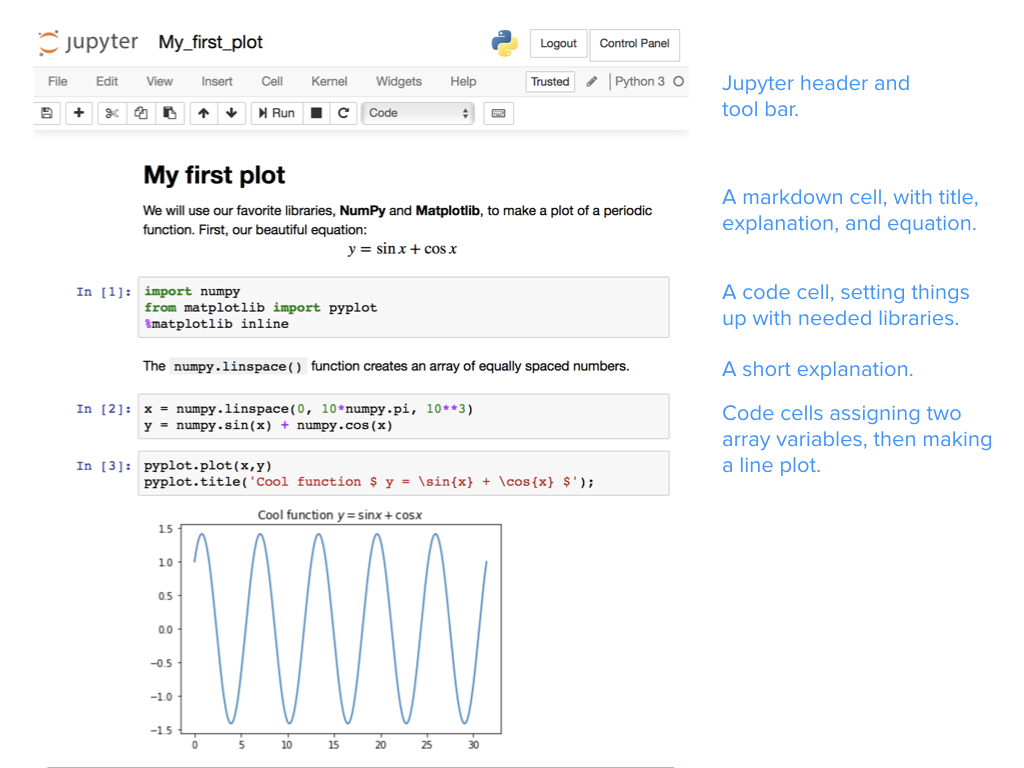
\includegraphics{images/Fig_notebook.png}
\caption{A Jupyter notebook, starting with a markdown cell containing a
title and an explanation (including an equation rendered with LaTeX).
Three code cells produce the final inline plot.}
\end{figure}

Jupyter is a free, open source platform that is an excellent learning
environment for students. For teachers, it increases our efficiency and
decreases cognitive load so we can engage students. Notebooks can be
useful for achieving your goals as a teacher in numerous environments
from STEM labs or humanities narratives, to podium lectures or flipped
classrooms. We use Jupyter notebooks in small classes and for classes
that have hundreds of students. Jupyter notebooks can be used for
teaching part of one lecture or can be used to teach a whole course.
Jupyter notebooks enable us and our students to have a conversation with
a problem and link to resources, like audio, video, images,
visualizations--and even allow students to mix and remix these. And yet
students need to install nothing beyond a modern web browser to use this
free software.

Jupyter notebooks can be used to organize classroom materials and
objects, store and provide access to reading materials for students,
present and share lecture materials, perform live coding, explore and
interact with materials, support self-paced learning, grade students'
homework, solve homework problems, or make materials reusable to others
(see Chapters 3 and 4).

Read on to find out how we have used Jupyter notebooks for teaching and
learning to benefit both our students and ourselves. Jupyter notebooks
support a wide range of learning goals, including learning to program,
learning domain knowledge, and practicing communication skills like
storytelling. The authors of this book have used Jupyter notebooks to
teach:

\begin{itemize}
\tightlist
\item
  Sciences

  \begin{itemize}
  \tightlist
  \item
    Physics and astronomy
  \item
    Geoscience
  \item
    Biology
  \item
    Cognitive Science
  \item
    Computer science
  \item
    Data science
  \item
    Statistics
  \item
    Social sciences
  \end{itemize}
\item
  Writing

  \begin{itemize}
  \tightlist
  \item
    Writing Seminar
  \item
    Writing and technical communication
  \end{itemize}
\item
  Digital Humanities

  \begin{itemize}
  \tightlist
  \item
    Music
  \item
    Text analysis
  \item
    Metadata processing
  \end{itemize}
\item
  Engineering

  \begin{itemize}
  \tightlist
  \item
    Chemical engineering (kinetics and reactor design)
  \item
    Mechanical engineering
  \item
    Aerospace engineering
  \end{itemize}
\item
  Introduction to Programming

  \begin{itemize}
  \tightlist
  \item
    High school
  \item
    College and university-level courses (true introductions through
    advanced courses)
  \end{itemize}
\end{itemize}

Our other use of notebooks for education include:

\begin{itemize}
\tightlist
\item
  Building models/simulations (with and without programming)
\item
  Using widgets to demonstrate and interact with simulations
\item
  Visualizations of process and data
\end{itemize}

\section{Course benefits \& anecdotes}\label{course-benefits-anecdotes}

\subsection{Engagement}\label{engagement}

As teachers we routinely struggle to engage our students, especially
when we are constrained by the format of the course (e.g., online,
50-minute lecture), available technologies, students distractions,
and/or other factors. Nevertheless, it is substantially our
responsibility to create environments and experiences within these
limits that engage students in our courses. This is where notebooks can
give you another tool to break out of the mundane, and get students
engaged in their learning.

\subsubsection{Conversations with data}\label{conversations-with-data}

The creators of Jupyter describe it as a set of open-source tools for
interactive and exploratory computing, and a platform for creating
computational narratives. Jupyter allows us, as educators, to narrate a
``conversation between the student and data''. Consider this example,
using the data of life expectancy of many countries over the years:

\begin{quote}
I use a short bit of code to make a graph showing the time evolution, in
what is called a ``spaghetti plot'' (see figure). Looking at this messy
graphic, I point out how most of the lines show growth over time: life
expectancy is improving all over the world. But a couple of lines show a
marked dip in a given year. I can ask students: which country had that
dip? What happened there? Why? With a bit more coding, we identify that
Cambodia had a shocking life expectancy of about 30 years in 1977, and
Rwanda had even worse life expectancy in 1992. We then have the
opportunity to discuss why these countries experienced a mortality
crisis. The data brings to life a meaningful discussion, with many
possible paths involving history, politics, economics, and health. --
Lorena Barba
\end{quote}

\begin{figure}
\centering
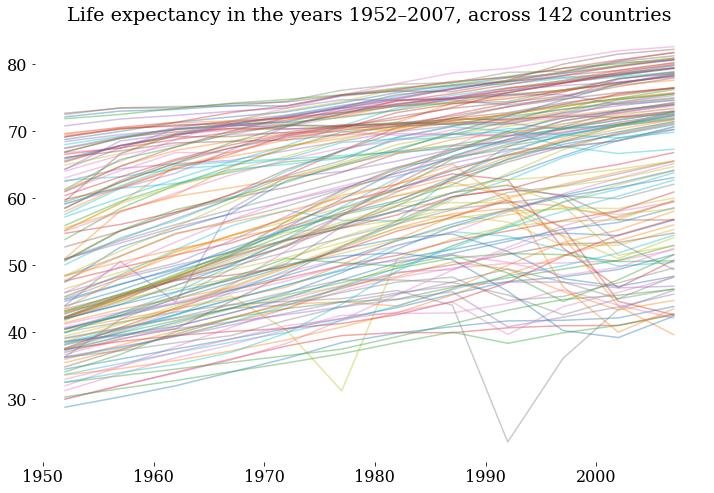
\includegraphics{images/engcomp2lesson4-life-expectancy.png}
\caption{From: \url{http://go.gwu.edu/engcomp2lesson4}}
\end{figure}

Jupyter notebooks are essential tools of connection---tools that engage
learners in transitions in their thinking. The opportunity of
intermingling computation into a narrative, creating a conversation with
data is a powerful and effective form of communication. With Jupyter,
you now have a new form of content to create and share with learners:
\emph{computable content}. In a world where every subject matter can
have a data-supported treatment, where computational devices are
omnipresent and pervasive, the union of natural language and computation
creates compelling communication and learning opportunities.

\subsection{Participation}\label{participation}

Engaging students in your courses requires their participation and
interaction with you, their peers, and/or the content (M. G. Moore,
\protect\hyperlink{ref-moore1989three}{1989}). How, when, and why you
use student participation in yours will, of course, depend on your
goals, the specific objectives for teaching the content within your
course, your students, and other factors. Using notebooks, however,
encourages participation and gives you more tools for promoting
participation. Notebooks can connect students to authentic external
audiences as well. Students can, for example, consume notebooks from
other classes, and publish notebooks where others can read them.

\subsubsection{Real world experience -- bringing concepts to
life}\label{real-world-experience-bringing-concepts-to-life}

Notebooks are living documents, meaning they can be edited to respond to
questions or input from students and used a conversation piece during a
lecture or presentation.

\begin{quote}
Our group uses Jupyter notebooks as ``apps'' to demonstrate concepts in
geophysics. These notebook-apps connect numerical simulations to widgets
and relevant plots. In the classroom, we ask students to help define
input parameters based on an application or case study that they are
interested in. Prior to displaying the results, we ask students to build
a mental image of their expectations. If the resultant image matches
their expectations, then we have reinforced a concept, and if not, it is
an opportunity to learn. We as instructors can interactively engage with
students' questions by updating the inputs to the simulation in order to
explore concepts with them. Students have access to the same notebooks
through free web-platforms like Binder, so simply by following a link,
they can take the steering wheel and engage with the concepts on their
own. Notebooks bring the concepts to life and serve as a conversation
piece for the interaction between learners and educators. -- Lindsey
Heagy
\end{quote}

\begin{figure}
\centering
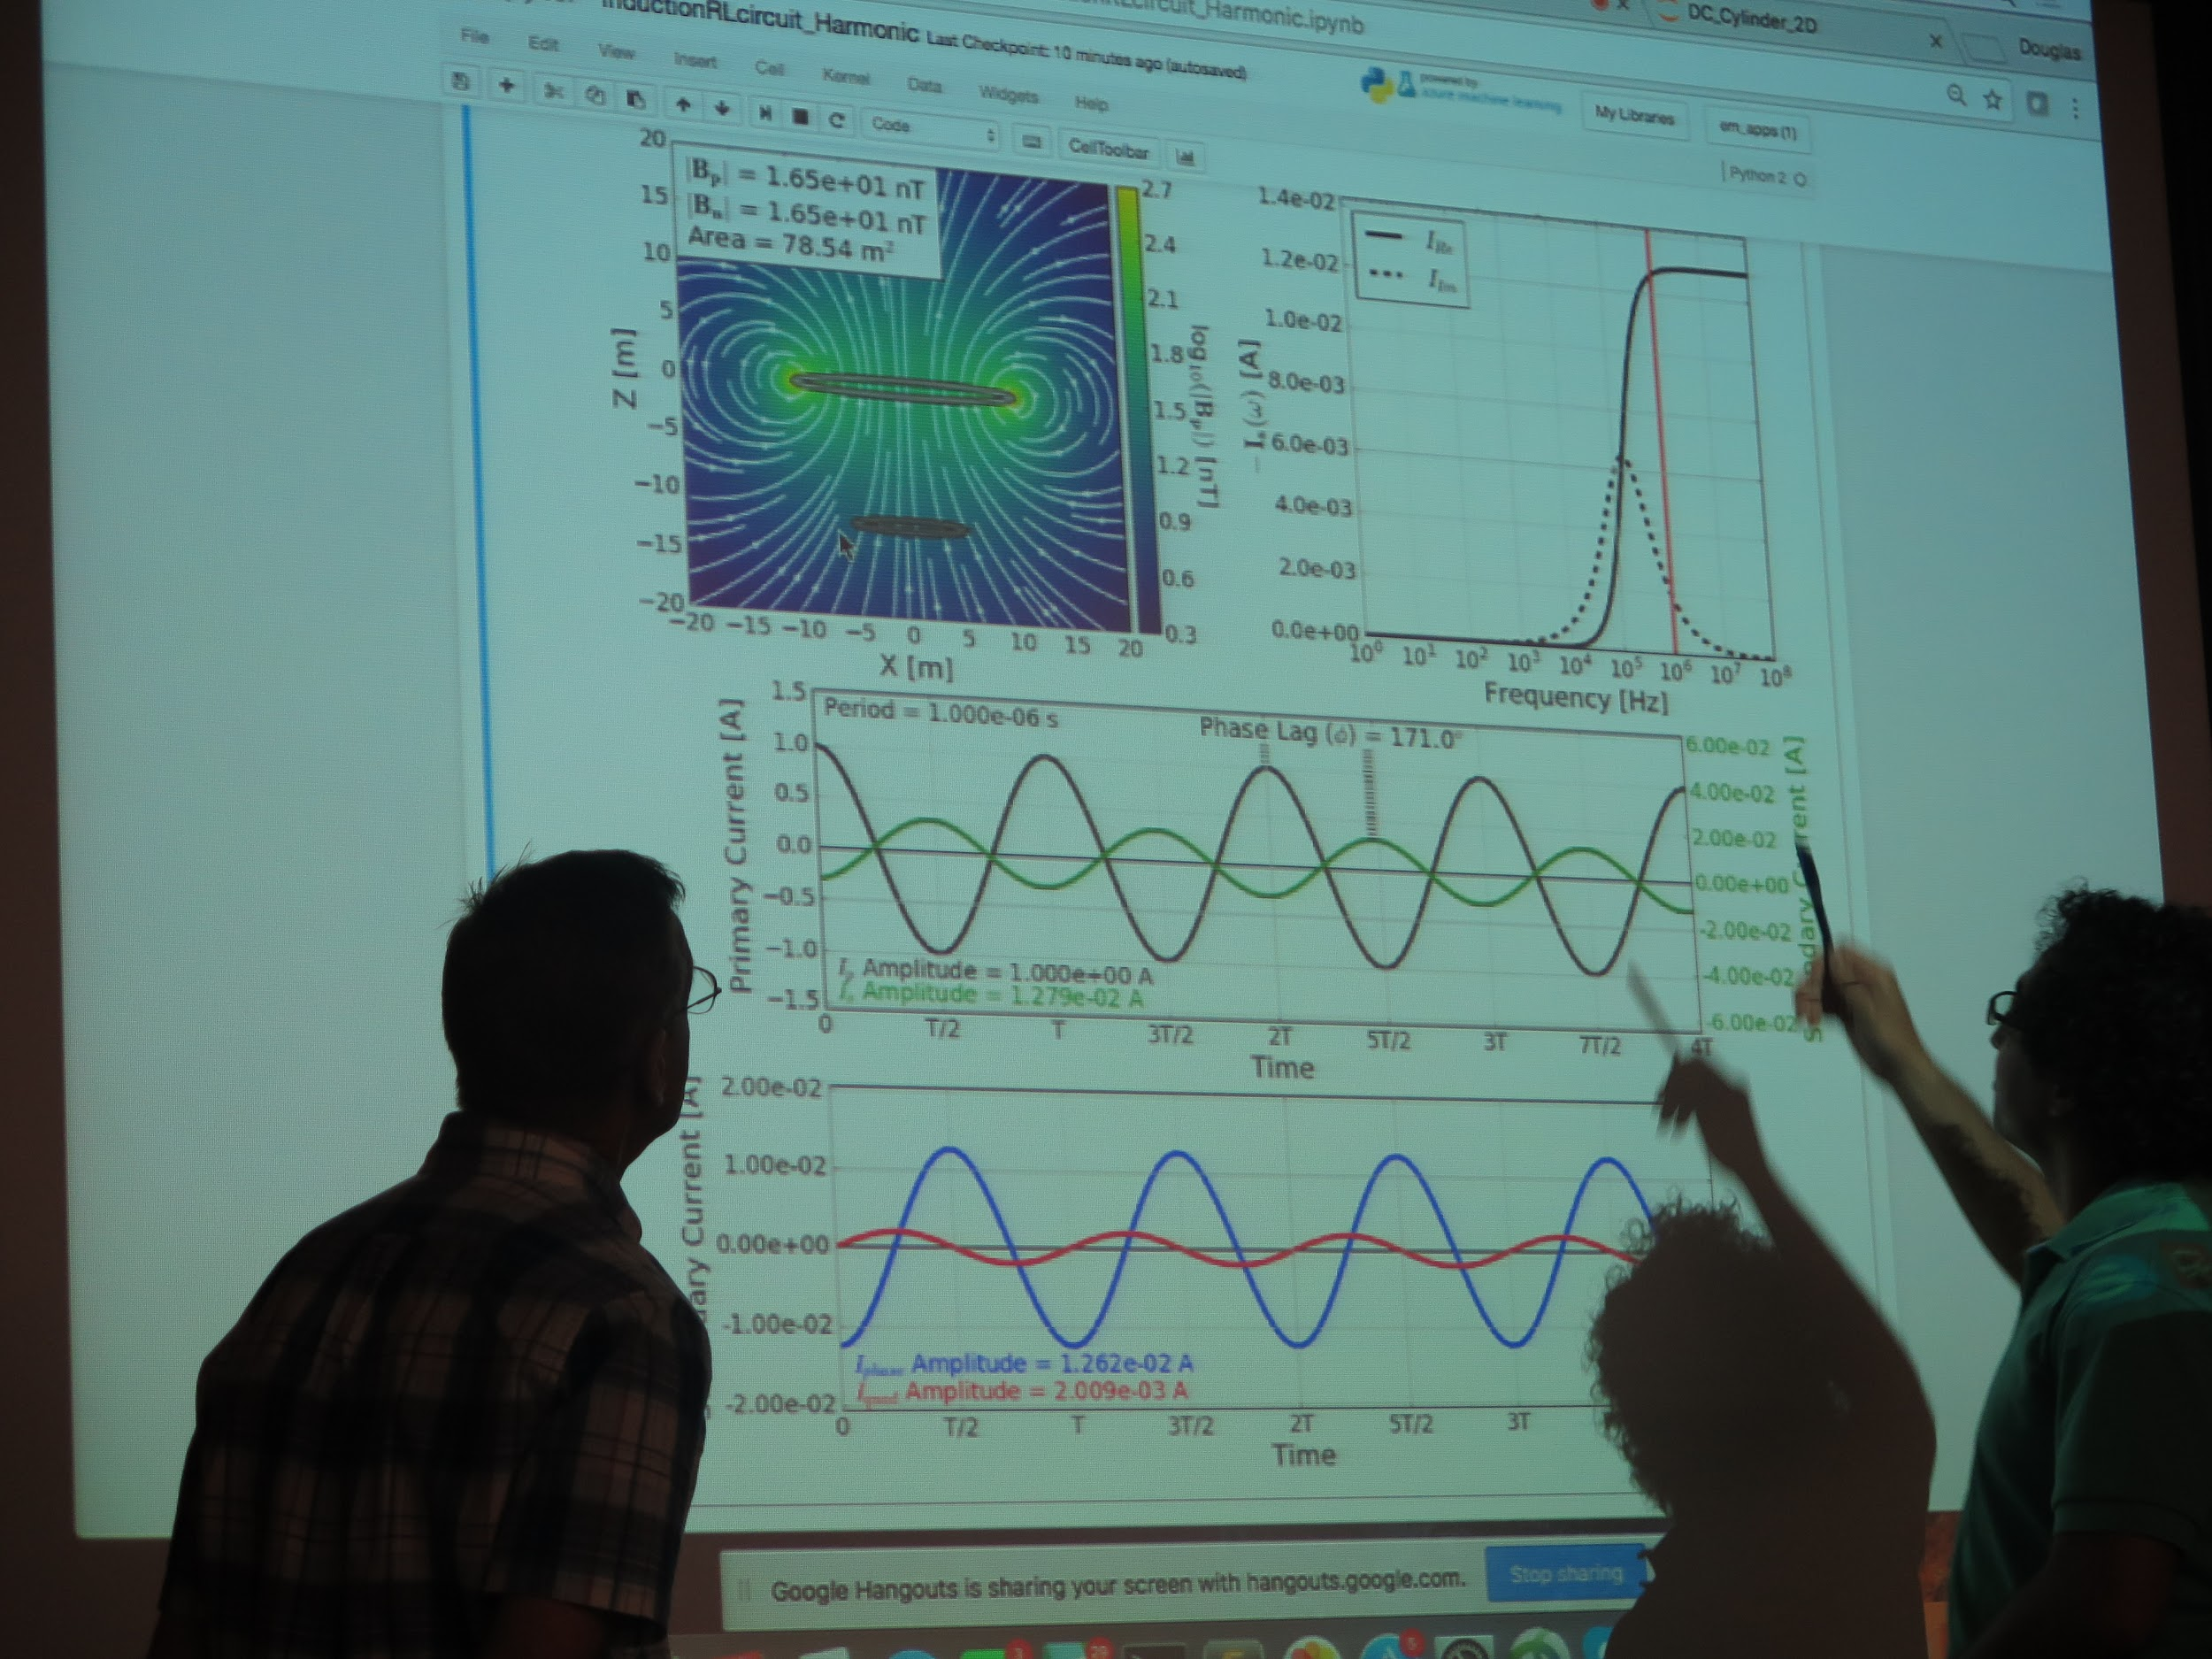
\includegraphics{images/oldenburg-geosci.jpg}
\caption{Dr.~Douglas Oldenburg (left) engaging with a student during a
short course on geophysical electromagnetics (\url{https://geosci.xyz}).
Photo credit: Seogi Kang}
\end{figure}

\subsubsection{Real world experience -- Ticket to
leave}\label{real-world-experience-ticket-to-leave}

Another example of generating participation in the classroom with
Jupyter notebooks is the Activity magic, available as an extension. It
creates what has been called a ``ticket to leave'' (or ``exit ticket'')
via the notebook. The idea of a ``ticket to leave'' is an excellent way
to end a class or lab. Briefly, it is just a survey that you give the
students (see figure). Often, these surveys are given via a Personal
Response System (also known as ``clickers'' or PRS) or cell phones.
There are a few uses of such surveys:

\begin{enumerate}
\def\labelenumi{\arabic{enumi}.}
\tightlist
\item
  Give the instructor some feedback on the students' understanding, as a
  whole
\item
  Provide time and opportunity for students to review and synthesize
  today's materials
\item
  Allow the students to apply their recent knowledge to a novel problem
\item
  An additional instance to learn the materials
\end{enumerate}

\begin{figure}
\centering
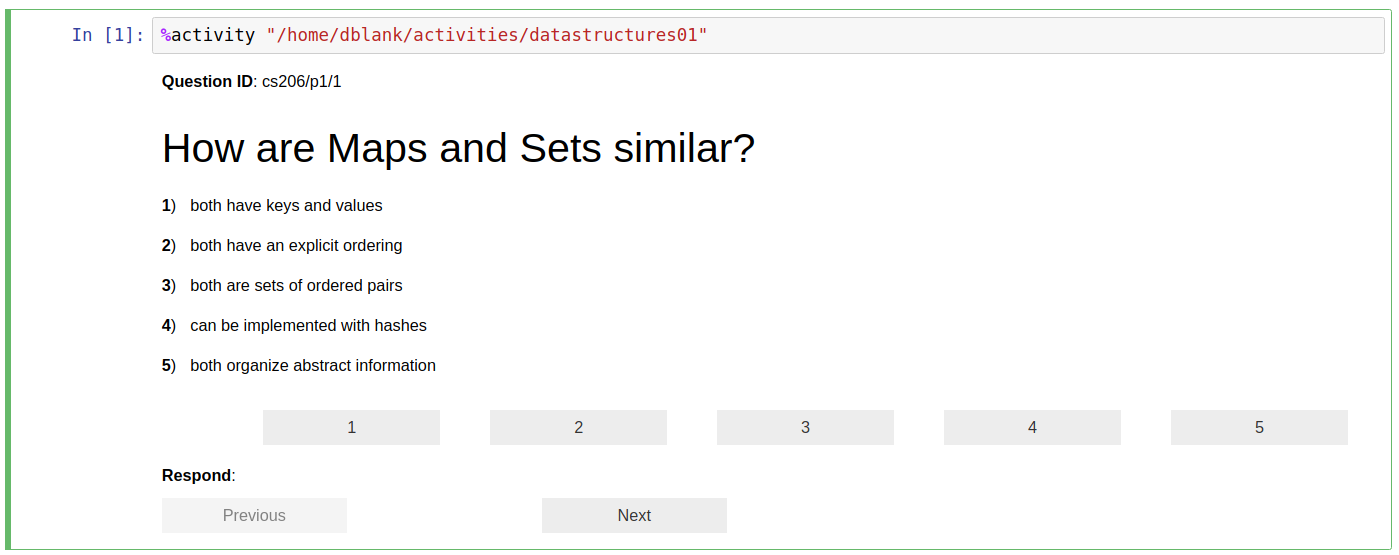
\includegraphics{images/activity-magic-student.png}
\caption{Example of the Activity magic seen from the students view. A
question, with multiple choice answers is shown, with buttons for their
input.}
\end{figure}

These questions do not typically require much time to answer, but are
meant to capture the essence of the conversation of the class. After a
minute or so to contemplate the question, the students select their
answer (by clicking one of the buttons), and instructor shows the
gestalt results (see figure).

\begin{figure}
\centering
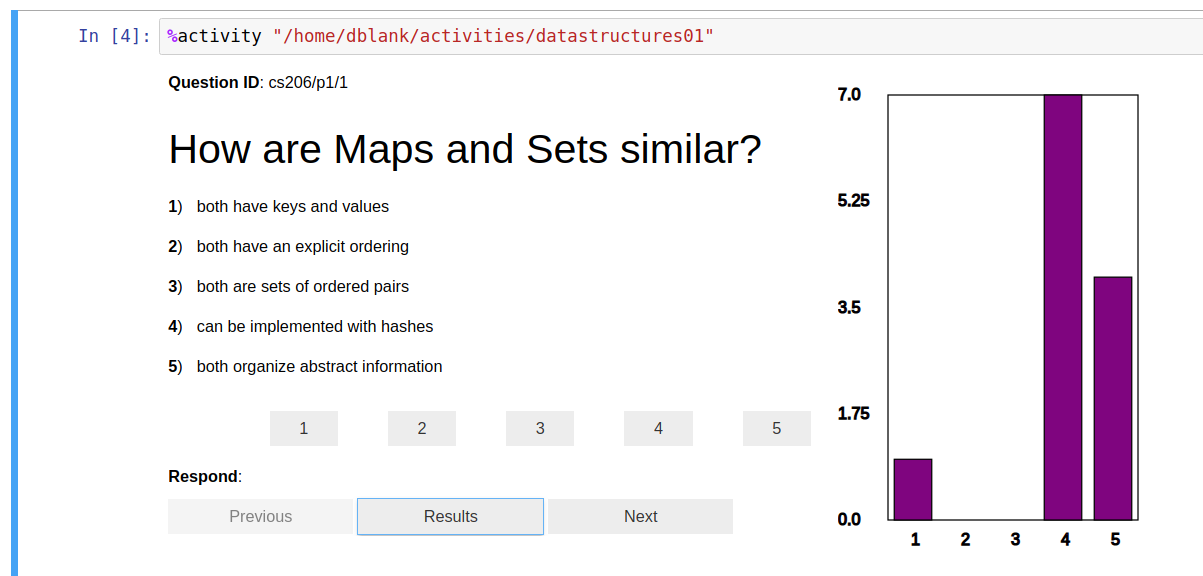
\includegraphics{images/activity-magic-instructor.png}
\caption{The Activity magic, from the the instructor's perspective. The
barchart is shown on the projector once all of the students have had a
chance to respond.}
\end{figure}

Good ``exit ticket'' questions can be domain specific questions, but can
also be metacognitive questions (about one's learning style, for
example), or high-level organizational questions (e.g., ``what was the
goal of today's discussion?''). We recommend leaving enough time at the
end of class (perhaps 10 minutes) to have a full and complete wrap-up
discussion. After the discussion, you may wish to adjust the following
class meeting if you feel that not enough students had the insight you
were aiming for. For more information on ``tickets to leave'' see
\url{https://www.brown.edu/sheridan/teaching-learning-resources/teaching-resources/course-design/classroom-assessment/entrance-and-exit/sample}.
For more on the Jupyter Notebook extension, see
\href{https://github.com/Calysto/metakernel/blob/master/metakernel/magics/README.md\#activity}{using}
and
\href{https://github.com/Calysto/metakernel\#use-metakernel-magics-in-ipython}{installing}
Calysto Activity magic.

\subsection{Increasing understanding}\label{increasing-understanding}

Within any course you will typically try to achieve a diverse set of
objectives. Benjamin Bloom
(\url{https://en.wikipedia.org/wiki/Bloom\%27s_taxonomy}) provided a
framework for the detailed objectives we want to achieve, ranging from
basic knowledge (such as, terminology, specific facts, trends and
sequences, classifications and categories, etc.) all the way to ability
to evaluate and create (such as, abstract relationships, judgments but
based criteria, original works). Achieving the former (i.e., basic
knowledge and comprehension) is far easier to achieve than understanding
(i.e., evaluation and creation); yet, most often we, as educators, are
striving for increasing the complex understanding of our students on the
topics we are teaching. The good news is that notebooks offer a valuable
tool for teaching toward understanding -- moving students, for example,
from passively viewing course content to exploring, analyzing,
synthesizing, and evaluating the content in active ways.

\subsubsection{Real world experience -- Guiding learners at their own
pace}\label{real-world-experience-guiding-learners-at-their-own-pace}

The fundamental theory behind Computational Fluid Dynamics (CFD) used in
Aerospace Engineering is based on understanding the Navier-Stokes
equations. ``CFD Python'' is a collection of Jupyter notebooks based on
a practical module that Lorena Barba began using in class in her
Computational Fluid Dynamics (CFD) course at Boston University in 2009.
The 5-week module develops worked examples that build on each other to
incrementally guide the learner to create a program to solve the
Navier--Stokes equations of fluid dynamics, in 12 steps.

\begin{quote}
In 2013, I was invited to teach a 2 day mini-course in the
Latin-American School in High-Performance Computing, in Argentina. The
Jupyter notebooks platform allowed me to create a guided narrative to
support learners with different background experience and knowledge. For
that event, we wrote notebooks based on the CFD course module, to use as
instructional scaffolding in the minicourse. Twenty students worked
through the notebooks as self-paced lessons, while I went from desk to
desk asking and answering questions. About four of the students
completed all 12 steps in the 2 days, a bulk of them achieved up to
about Step 8, and a few of them lagged behind in Steps 4 or 5 by the end
of the course. For those who completed the full module, they had
achieved in 2 days what my regular students in the classroom normally
took 5 weeks to do. Seeing that was an eye-opening moment: both the
power of worked examples in code, and the ability to allow learners to
follow their own pace made a remarkable difference in these learners. --
Lorena Barba
\end{quote}

Based on the experience developing the ``CFD Python'' learning module
(Barba \& Forsyth, \protect\hyperlink{ref-barbacfd}{2018}), this basic
design pattern was adopted for creating lessons using computable
content:

\begin{enumerate}
\def\labelenumi{\arabic{enumi}.}
\tightlist
\item
  Break it down into small steps
\item
  Chunk small steps into bigger steps
\item
  Add narrative and connect
\item
  Link out to documentation
\item
  Interleave easy exercises
\item
  Spice with challenge questions/tasks
\item
  Publish openly online
\end{enumerate}

This was particularly helpful for student understanding.

\subsection{Increasing student's
performance}\label{increasing-students-performance}

The goal of learning is often actualized through the performance of
students. This is routinely most visible by what we attempt to assess
during and at the end of instruction. Using notebooks we can create a
variety of a performance opportunities for students, thereby giving them
more opportunities for practice and feedback, as well as more
opportunities for us, as instructors, to assess their ability to
perform.

\subsubsection{Real world experience -- The worked-example
effect}\label{real-world-experience-the-worked-example-effect}

The worked-example effect is the best known and most widely studied of
the cognitive load effects (Sweller,
\protect\hyperlink{ref-sweller2006worked}{2006}). It refers to providing
full guidance on how to solve a problem, resulting in better student
performance than problem-solving conditions with no guidance. For
complex tasks, inexperienced or beginner learners benefit the most from
the worked-examples procedure. One study (Chen, Kalyuga, \& Sweller,
\protect\hyperlink{ref-chen2015worked}{2015}) concludes that: ``worked
example effect occurs for complex, high-element interactivity materials
that impose a heavy working memory load'' and ``when dealing with
complex material that learners may have difficulty understanding, high
levels of guidance are likely to result in enhanced performance over
lower levels of guidance.'' This research-based guidance seems
especially relevant for teaching novice programmers to use computation
in the context of their subject matter (science, engineering, or other).

\subsection{Increasing students' preparation for their
career}\label{increasing-students-preparation-for-their-career}

In preparing students to apply what they have learned, striving to align
what happens in the course with what they will experience in their
career is important. From using parallel software to mirroring
workflows, we want our students to experience and be prepared for the
workplace. Recognizing, of course, that workplaces are not static and
the skills required for a career are always emerging, using notebooks
provides a flexible platform to build skills and build portfolios of
what students can do.

\subsubsection{Real world experience -- Publishing a data narrative as a
demonstration of industry
ability}\label{real-world-experience-publishing-a-data-narrative-as-a-demonstration-of-industry-ability}

For Data Science careers, a publicly shared narrative about a data
analytics project goes a long way at demonstrating the student's
potential at an interview. Elizabeth Wicks has her students develop a
Jupyter notebook that tells the story of a data munging and analysis
project done in the class. The students then publish this notebook to
their Github profile pages. Being that Jupyter is one of the most
popular ways in industry to communicate data science results, the
students have a very valuable key to a potential career.

TODO: Add quote from Elizabeth

\section{Student benefits}\label{student-benefits}

Creating opportunities for students to develop as learners stretch
beyond the boundaries of any specific course where you may use
notebooks. By enriching their learning experience in your course, you
will help them develop valuable skill-sets and mind-sets that they will
take with them into other courses and into their career.

\subsection{Computational thinking}\label{computational-thinking}

Jupyter notebooks support a wide range of learning goals. Its
interactivity enables building intuitive understanding of domain
knowledge, such as the understanding of a mechanical response of a
system while varying parameters or understanding how an algorithm
behaves. Notebooks can also help teach effective communication skills,
combining prose with graphics into a strong narrative. Finally,
notebooks can support teaching or strengthening programming skills, by
combining code with text descriptions and visualizations. Even if a
notebook is designed to be consumed passively, the exposure to code
helps show students how to do something---and that they can do it
themselves. This also helps demystify coding for students who do not
view themselves as traditional ``computer science'' types.

Using notebooks, you can create rich learning experiences that link
together the core foundations of computational thinking:

\begin{itemize}
\tightlist
\item
  \emph{Decomposition}: Breaking down data, processes, or problems into
  smaller, manageable parts
\item
  \emph{Pattern Recognition}: Observing patterns, trends, and
  regularities in data
\item
  \emph{Abstraction}: Identifying the general principles that generate
  these patterns
\item
  \emph{Algorithm Design}: Developing the step by step instructions for
  solving this and similar problems
\end{itemize}

\subsection{Open-source}\label{open-source}

Integrating notebooks into classes also exposes students to a large and
growing ecosystem of open-source tools. This supports their education,
but also provides experience in the same environment of tools used in
industries in high demand for trained employees, such as data science
and machine learning. The open-source nature of these tools also ensures
that course content remains accessible and affordable to all
students---including those outside the traditional university
environment.

Unlike proprietary notebook technologies such as Mathematica, or
specific programming languages/environments such as Matlab or C++, the
barriers to entry for students learning with Jupyter notebooks can be
extremely low. At a minimum, during a lecture, students can simply
watch/read an interactive demo using a notebook, to replace slides or
lecture notes. On their own, using a cloud service such as Binder or
JupyterHub, students can open any modern web browser to some address and
interact with a notebook (an example of this technology can be found at
\url{https://jupyter.org/try}), without needing any installation or
configuration. In the most complicated case, students can install
Anaconda and follow simple instructions to install the Jupyter Notebook,
which works and looks the same on all platforms---and is free and open
source.

\subsection{Active learning}\label{active-learning}

Thanks to their interactivity, notebooks enable a spectrum of active
learning methods, which have been shown to increase performance in
science, engineering, and mathematics (Freeman et al.,
\protect\hyperlink{ref-freeman2014active}{2014}). To start, students can
consume notebook content by reading and running notebooks, then move to
editing or completing notebooks as assignments. This allows students to
focus on the content and concepts, rather than just note-taking.

At the top of Bloom's Taxonomy is pure creation, where students can, for
example, author complete computational essays. In both cases, notebooks
support courses where students have a wide range of experience and
ability: students who need help can rely on the scaffolding of prose
explanations and existing code, while also providing room to stretch and
explore for more-experienced students. The additional annotation and
prose that accompanies code also helps support non-traditional learners
and students from underrepresented groups who may have less initial
experience/comfort with programming.

Instilling the habits of active learning, through the use of notebooks,
will also provide benefits beyond the boundaries of your course.
Interactivity drives engagement, interest, and exploration of concepts.
Engaged students in your course are more likely to be engaged learners
in other courses and beyond.

\section{Instructor benefits}\label{instructor-benefits}

Notebooks can be adopted at a variety of levels and formats, offering
flexibility based on the needs of a course and comfort/interest level of
the instructor: in-class demos, interactive labs, auxiliary material
(e.g., book replacements, lecture note supplements), assignments, or
full course content in a flipped learning environment. Notebooks offer a
route to active learning methods for instructors without experience of
them, but do not force a particular teaching style.

At a minimum, notebooks can be used to make publishable and interactive
lecture notes that blend narrative text, images, videos with image and
results to present the concepts. Furthermore, these course materials can
be developed gradually, starting with a low-effort draft to a
more-polished, publishable document that can be easily extended over
time---and adopted by others. The growth of open-source communities
around software tools and educational resources creates more
opportunities for the re-use and adaptation of existing resources.

While many notebook authors do use Python, the Jupyter Notebook supports
many languages, so students (and instructors) are not tied to one
specific language. Indeed, the name Jupyter comes from three languages:
Julia, Python, and R. Furthermore, these (free) tools have minimal
barriers to entry---using a cloud infrastructure means students and
instructors do not have to install anything, while in the ``worst'' case
installations require a few command-line excursions, but these are free,
openly available, and cross-platform.

\section{Conclusions}\label{conclusions}

We hope that this chapter has illustrated that teaching with Jupyter
notebooks can be valuable for you and your student. We have shown
notebooks to be a tool that can increase student engagement,
participation, understanding, performance, and preparation for their
careers. These are substantial accomplishments that can be achieved in a
variety of disciplines and content areas. Using several real world
examples, we attempted to illustrate the numerous ways teachers are
using notebooks. Hopefully these, when combined with the chapters that
follow, will guide you in 1) supporting your students' learning, 2)
giving you confidence that you can use notebooks, 3) help you understand
the necessary logistics, and 4) help give you clear expectations of what
can be accomplished with Jupyter notebooks.

\chapter{Notebooks in teaching and
learning}\label{notebooks-in-teaching-and-learning}

Jupyter notebooks are a valuable tool for teachers, but their value can
only be leveraged if you apply them correctly within the context of your
course. In this chapter, you will learn how teachers can initially
structure the design of their course and then determine when and how
notebooks can be used to achieve their goals.

\section{Oh the places your notebooks will
go!}\label{oh-the-places-your-notebooks-will-go}

\subsection{Introduction}\label{introduction}

In Chapter \ref{catalogue} you will learn about the many creative ways
that notebooks can be used within the design of your course. Many times
notebooks can be adapted into course activities that you are already
doing, and other times notebooks will give you opportunities to extend
what you have done in past to increase the engagement, participation,
understanding, and performance of your students. Jupyter notebooks can
be a valuable member of your existing instruction toolkit, useful at
every point in the learning environment. New adopters of Jupyter can
start small, incorporating notebooks into single modules, assignments,
or classroom activities. This is an excellent approach to see how your
learning audience interacts with the notebook environment and explore
notebook hosting systems in a low cost/risk way.

Instructors adopt Jupyter within their classrooms at a variety of
levels, each making use of the strong features of the environment.
Transitioning an existing course to any new platform seems daunting, but
Jupyter notebooks are modular and ideal for an iterative development
approach of adoption. Some may find themselves inheriting a course
already built in Jupyter, while others will choose to build new courses
entirely within Jupyter.

This section seeks to inspire you about the many uses of Jupyter within
classroom content and presentation design, and preview how other
elements of the Jupyter ecosystem can be integrated into that use. Some
of these uses are quick to spin up as experiments to test the waters.

\subsection{Jupyter notebooks as
textbooks}\label{jupyter-notebooks-as-textbooks}

Instructors often write Jupyter notebooks as linear narrative documents.
These notebooks are to be read by students and learners, perhaps worked
through, marked up and are a relatively one sided information
consumption experience.

Most often these notebooks exist as the readings a learner is required
to do before class, as reference material (e.g., to review for future
assessments), or something that a learner works through on their own as
a part of self study. Jupyter notebooks can be constructed of completely
static text, which can serve as a starting point for transitioning
existing material into the notebook environment.

This traditional static textbook chapter or section can be extended into
an active space by changing inline code text to executable code cells
that support modification and experimentation. Adding prompts with
suggestions for interrogating the code and examples further extend
active learning opportunities without rewriting the original content.
Interactive sliders, user input sources, and manipulable visualizations
are examples of how other widgets and plugins can open up more
possibilities.

As you'll see in later chapters, many authors are using Jupyter
notebooks as their primary authoring and publishing platforms. These
materials are published on paper and online, meaning that the
interactive portions of the learning experience are first class elements
within the resource.

\subsection{Notebooks as
workbooks/primer}\label{notebooks-as-workbooksprimer}

Workbooks engage students in the notebook environment by including
active elements where they are asked to manipulate or create new
content. This moves students from a passive or static learning
environment like a book into an active learning experience where they
can engage with and critically think about the content.

You can include many pedagogical patterns (discussed in the
\protect\hyperlink{catalogue}{next chapter}) within a workbook, crafting
a completely custom learning experience. These workbooks can be assigned
as independent student learning (for example, pre-work for flipped
classroom), or as part of an in class activity for individuals or small
groups.

When teaching in the technical space, the exploration of concepts in
their context is an ideal environment for showcasing an authentic
experience to students. Studying a concept in isolation may reduce the
complexity of the problem to be more accessible, but this removes it
from the context for why it exists and may make it harder for students
to put all the pieces together and synthesize it into their larger
problem solving repertoire.

Retention of this context adds the complexity of expository text,
technical reference in disconnected documents, or some boilerplate code.
Providing this in a large script or lengthy lists of direction can be
overwhelming for students to work with. Jupyter notebooks are excellent
tools for teaching these complex workflows, because instead of a script
with lengthy code comments or having disconnected documentation, this
guiding text can be embedded exactly where it is needed where the coding
is happening. This guidance material can also be formatted as markdown
cells, which are visually distinct from code, making it easier to
visually scan and opens the possibility to add helpful formatting.

A variety of activities can be supported with the executable code cells
so learners can explore the space in an interactive and iterative
environment. They can see and inspect portions of the surrounding code,
but aren't required to touch it, maintaining appropriate granularity for
assignments and challenges. Using markdown formatting separating
sections helps scaffold larger problems and help them really experience
a real world workflow rather than statically read about it.

\subsection{Notebooks as worksheets/drill
sets}\label{notebooks-as-worksheetsdrill-sets}

Many programming and domain tasks have specific syntaxes to be learned
and effectively memorized before they can be internalized. Akin to math
homework sheets, short worksheets where learners focus on highly
granular or decontextualized problem sets lets them practice the complex
syntax and procedures in an isolated and highly focused way. A set of
small targeted tasks where these complexities can be practiced without
the worry of additional syntax errors or other problem solving
requirements can reduce the cognitive overhead a student might be
overwhelmed by.

The cell based nature of the Jupyter notebook makes interactive
code-based worksheets a clean experience for students to run. Each
problem prompt can be written in a markdown cell, perhaps referencing an
object or data file established in an initial cell. For example, a list
or other data structure would be defined at the top and the exercises
below are focused on the relevant methods and usage syntax. Each answer
would then be completed by the student in a single code cell just below
that markdown cell. This means that outputs and errors stay with the
code producing them, so successes or bugs are easily traceable to the
source.

Usages of autograding tools or unit tests, as discussed in later
chapters, can be added to give students instant feedback about their
work. Example or desired outputs could also be reproduced in markdown
cells with the question for further guidance.

\subsection{Notebooks as notepaper or course
packets}\label{notebooks-as-notepaper-or-course-packets}

The ability for a notebook to represent a linear experience with human
prose and working code means that these can be used a student's
notepaper in class. They can capture the linear narrative structure of a
lesson or lecture, and actually run the code they are taking note of.
This ensures that what they have written down actually works, and makes
for a strongly reusable document for them moving forward with homework.

Encouraging students to use Jupyter notebooks for taking class notes
opens up further opportunities to provide scaffolding and support within
the classroom. Providing notebooks with outlines of lecture content or
other materials covered in class can become an useful active learning
and engagement strategy. You might provide a mostly blank notebook with
just topic headings, and ask them to take notes in their own style
within those spaces. Or you could choose to embed reference notes,
examples, and even small activities within the notebook, asking them to
both take notes and work through examples with you.

Caution should be taken to encourage students to carefully maintain a
linear order of their code in the notebooks. A later chapter has more
information on Jupyter specific caveats that students should remain
aware of.

\subsection{Notebooks as an app}\label{notebooks-as-an-app}

Notebooks even have a place in non-coding classroom content or activity.
Interactive user inputs like mouse or touchscreen controlled sliders,
buttons, highlighting, etc. allow a notebook user to manipulate input
parameters for a visualization, tool, or model without directly editing
any of the code within the notebook. These strategies support
interactive computational exploration, or transform the notebook into an
advanced calculator tool for students to use within their homework.
These notebooks are then treated as applications that are distributed or
made available for students to use during class or explore on their own.

This allows you to make an existing research workflow accessible to
novice students as part of a computational module of a foundational
class, or mock up content from a static textbook or reading into
something for an active learning activity. The adaptability and reuse
aspects of Jupyter notebooks also create opportunities for students to
take this code further and adapt it for assignments or other research.

\subsection{Notebooks as lab reports or
assignments}\label{notebooks-as-lab-reports-or-assignments}

There are a variety of assignment deliverables that programming and
technical courses may require. Students may be asked to produce essays,
presentations, working code, analytics, and even art or music. Many of
these deliverables are directly supported within the notebook
environment. Any written work could be completed within the notebook
environment with markdown, which is ideal for communication content that
is driven by data or incorporating code content. For example, a student
could write a computational essay within a notebook, and use one of the
presentation tools to present a report out in class, all using the same
notebook.

Coding assignments can be submitted to a Jupyter supported learning
management system and be autograded (discussed in later chapters),
providing instant feedback and automating the grading process. This
opens up self paced and highly scaled options for many courses,
particularly open access MOOCs or large sections. Meanwhile, the inline
visualization options mean that an assignment with graphical output can
be self contained without trying to embed images within a word
processing document or attaching a collection of images along with a
script.

The multiple conversion and hosting options available to notebooks means
that they can be shared or submitted across many formats. For example,
conversion to HTML means that there is zero overhead for viewing the
content, and support for markdown and PDF opens up accessibility and
other publishing platforms.

\subsection{Notebooks as interactive multimedia
platforms}\label{notebooks-as-interactive-multimedia-platforms}

A variety of media formats can be embedded within a notebook, and other
tools more offer platforms to more directly connect notebooks with
multimedia content. Instruction content might be split up between short
videos (often for flipped classrooms) or a variety of static images
might be important for an assignment. The markdown cells within the
Jupyter notebook provide several ways to place hyperlinks and embed a
variety of media.

Several widgets are also available for embedding playable audio and
video content (including from streaming video services) directly within
the notebook. This creates a cohesive platform experience for the
student, so they don't have to exit out or change screens to work on
their assignment and reference that content.

Other tools are available for more directly connecting the notebook
content to a video guide. Video lectures or content in your courses can
get lengthy in running time and associated notebooks are often just as
long. Tools like
\href{https://www.safaribooksonline.com/oriole/}{Oriole} provide a
platform where you can integrate video timestamps into notebooks to
create interactive video experiences. You can include, for example,
Youtube videos within notebooks, with text and/or coding opportunities
before/after the video. Using timecodes, you can also guide students
through the videos in tandem with the notebook text. This further
extends the ability to create a single cohesive interactive experience
without the need for students to go back and forth between materials.

\subsection{Notebooks as a demonstration
platform}\label{notebooks-as-a-demonstration-platform}

Eventually you will have to display a notebook in class. This may be as
a demonstration of how to use a notebook, presenting more a traditional
style lecture, creating and editing code, or using an interactive
feature to explore an experiment. Normal standards for font sizes,
organization, and accessibility stand for these cases.

Displaying actual notebook within your presentation is a natural
starting point. This content may include text from markdown and LaTeX,
code, and independent figures and sketches. For instance the lecturer
could display the notebook, slowly scrolling through the material and
interacting with cells containing code while also making use of either a
digital or analog (e.g.~chalkboard) sketching device. Custom styling
plugins are available to change the background color, font, and other
viewing aspects of the notebook for better presentation quality and
accessibility.

Several slide show tools are available, which allow you to markup
notebook cell content for a more traditional slideshow presentation mode
without having to exit from your standard notebook. These slides can be
scattered across notebook content into specific cells that will
correspond to individual slides, with the other content ignored from the
presentation. This then can be shown alongside the usual notebook
interface and can be flipped between the other forms of content.

It is natural for students to read and interact with notebooks in their
standard form, using either Jupyter Notebook or JupyterLab, and this can
also be used for presentation. Jupyter Lab offers the convenience and
uniformity of being able to open and edit source files (\texttt{.py},
etc.) within the same environment and without OS- or browser-specific
clutter. Full screening the browser is recommended if presenting using
this mode. Presentation styles vary widely and span a spectrum from
full-prepared notebooks to blank-slate live coding.

Many find it useful to incorporate an alternate modality such as a
physical or digital ``board'' for free-form diagramming, working through
a mathematical derivation, or other written procedural task. Notebooks
can be a portion of these presentations or the complete environment,
depending on your personal instruction style and content needs.

Care should be taken about how the notebook is presented and
demonstrated. Doing a live demo gives you a few options. You might
choose to:

\begin{itemize}
\tightlist
\item
  Scroll through a notebook
\item
  Step through a notebook by executing the cells in order
\item
  Fill out details or values into a mostly complete notebook
\item
  Tweak or flesh out a notebook with some content
\item
  Add content to a completely blank notebook
\end{itemize}

Each of these strategies have a place within a classroom, and their use
should be informed by audience needs and learning goals. For example,
having a notebook with prepared challenges for the end of each module or
section, but with blank cells for the content gives you the opportunity
to develop code live within class, but within a structure that keeps
your workflow organized, and your formative assessments coded directly
into your presentation. Incorporating reference information can make
these documents more complete for students and answer common questions.
There are many possibilities about what you can put in. Keep in mind
that students will often ask for you to share copies of these notebooks
after the class session is completed.

How much you focus on live coding will likely be determined by the
domain content of the class. Programming courses would clearly have a
priority for students to have more thorough practice with writing and
typing in the code. However, a conceptual class looking at computational
models may interactively tweak parameters for a model and discuss only
what is happening within that mathematical model. No code is written or
directly changed in the process.

\subsection{Notebooks as a live coding
environment}\label{notebooks-as-a-live-coding-environment}

Live coding, as the name implies, involves the active writing of code
within the instruction process. This might be part of a recorded
screencast or an in person classroom. The process of live coding has
several benefits for the student and instructor.

Showing the process of building up code examples showcases the natural
non-linear process of how code is crafted, but walking through the logic
of a code example slows instruction down and highlights the reason for
inclusion of each element within the code.

Introduction of bugs (either purposeful or accidental) to the code has
the added benefit of giving the presenter an opportunity to work through
the debugging process and demonstrating that perfect code is never
created on the first go.

Live-coding can also be an opportunity to provide an active learning
experience by providing notebooks with code that has not been completed
before the lecture and having students attempt to fill in the missing
lines before doing the live-coding demonstration. Feedback on where
students are in this process can be a useful way to also judge what
students are retaining and are struggling with leading to just-in-time
teaching opportunities.

Formative assessment and prediction prompts can also be incorporated
either directly into the notebook or as part of the narration of the
lecture. Creating live-coding opportunities can be done anytime where a
block of code exists but picking out particularly illustrative examples
or key points and appropriately scaffolding the example can be critical.
For example, if the critical concept is inside of a for loop then only
coding the inner part of the for loop can be helpful and not overwhelm
the presentation with scaffolding such as the setup. The reverse can
also be true however. If too much complexity or scaffolding is displayed
learners may struggle to understand the scaffolding rather than
concentrating on the key concept.

Many instructors utilizing live coding will choose to have students code
along with them. This allows them to practice what they are learning,
see it in the natural context of their environment, make all the normal
mistakes and typos, and all within an environment where they can ask
questions (or pause a video). Actively coding along with the instructor
also includes a requirement that they are actively listening to the
instructor and engaged with the content.

Presentation styles of scrolling or shift + enter are not live coding,
but live demonstrations. While these limit or negate the benefits of the
live coding environment, the benefits of speeding up the presentation or
running through code that's irrelevant to the learning goals may be more
important. Removing the student's active engagement with the content may
eventually lead to their disengagement with the lesson, or missing large
chunks of information. Instructors should balance their inclusion of
live coding and live demonstration to ensure that students are active
and engaged with the most important aspects of the lesson.

Information bandwidth in the classroom during a live coding session
needs to be carefully managed, particularly when students are trying
follow along. The rhythm of live coding roughly has three stages:
preparation, typing, and explanation. These three follow quickly in
succession but are independent phases. Preparation is the first, where
you stop and explain what you are about to do. Typing is the next phase
where you should speak as you type but only say what you are typing.
This ensures that what the learners are seeing on the screen and hearing
from you match. They will likely be looking back and forth between their
screen and yours that they often won't be able to stop and follow what
you are saying while they are typing. The final stage is to stop and
explain what you have typed and what has or will happen when you run the
code. You may choose to execute the code and explain the results or
include a formative assessment or prediction question before running the
code. Pausing to explain the code you just wrote and walk through the
results gives students time to catch up to your typing, time to consider
what has happened, and a natural place to ask (and for you to as for)
questions about what has happened.

Live coding does take practice to get used to, but can be extremely
powerful for you to restrain your pace to your learners and to retain
engagement with your students.

\subsection{Conclusion about places}\label{conclusion-about-places}

As you have just seen, notebooks provide a flexible tool that can be
used in numerous ways to achieve your course goals. Notebooks are
flexible enough that you can use them from relatively passive to very
active student learning, you can use them in your lecture or in a
flipped-classroom environment. There is no single best way to use
notebooks in your courses, and you explore the various options you will
want to start filling your use of notebooks with a variety of the
pedagogical patterns described in the \protect\hyperlink{catalogue}{next
chapter}.

\section{Before You Begin\ldots{}}\label{before-you-begin}

This chapter focuses on course considerations when incorporating
notebooks into a class. Experienced instructors may choose to skim parts
of this chapter and focus specifically on how Jupyter notebooks would
change their current teaching style.

Before you begin adding Jupyter notebooks to your course, take some time
to:

\begin{itemize}
\tightlist
\item
  Identify your teaching goals
\item
  Understand your students
\item
  Develop your content strategy
\item
  Consider the context of the learning environment
\end{itemize}

The Jupyter notebook is a tool; its use in this context is subject to
the expectations of the instruction. Setting expectations for learning
depends on your goals, your students, the content, the learning
environment context, and you.

\subsection{Identify Your Teaching
Goals}\label{identify-your-teaching-goals}

As with the creation of a building or robot or book, it is important to
begin the process with a clear goal of what you are trying to create and
why. The ``and why'' could be the most important decision you make in
the whole process and it will (or at least it should) guide all the
decisions that follow. The why here is not about why to use Jupyter
notebooks, but the why is the goal you have for your students.

Is the goal to teach them critical thinking skills, or how to execute a
specific set of functions to solve a problem? Is the goal that they will
be able to translate mathematical concepts into real world application,
or is the goal to teach them how to code? Be specific and clear, and
then let the answers guide your decisions.

\subsection{Understand Your Students}\label{understand-your-students}

Your students are central to decisions about when and how to use
notebooks alongside other tools in your instruction. An obvious
illustration of these decisions would be selections made if you compare
teaching 5th graders in relation to teaching graduate students. Yet,
there are more subtle differences that you will also want to be aware of
and monitor. For example, within a classroom, you will have variation
among the backgrounds and skill levels of the students. Depending on the
domain, some students may have extensive experience with coding in
multiple languages while others may be doing their first computational
explorations. Keeping students of all different experience levels
engaged and excited is challenging.

\subsubsection{Learn About Your
Students}\label{learn-about-your-students}

In many circumstances you will have little background information on
your students prior to the first day of a class or workshop. You will
have to learn quickly and be prepared to adjust the instruction to fit
the students in attendance---not the students you wish you had or
anticipated having. Some key considerations to learn about your
students:

\begin{itemize}
\tightlist
\item
  \textbf{Motivation:} Why are your students participating? What are
  their goals beyond the workshop or class? Will they be applying what
  they learn soon, or not for months or potentially years?
\item
  \textbf{Entry skills:} What skills are students coming to the
  instruction with, both technical (e.g., basic computer, coding,
  computational) and psycho-social (collaboration, presenting, asking
  questions)?
\item
  \textbf{Prior topic knowledge:} Specific to the content of the
  instruction, what do they already know coming in?
\item
  **Attitudes toward \url{content:**} Are they excited to learn, or
  nervous about the content? How confident are they about their success
  in the class?
\item
  \textbf{Attitudes about the delivery format:} Do they have attitudes,
  positive or negative, about the delivery format (e.g., lecture,
  flipped classroom, lab) and/or technologies (e.g., learning management
  systems)
\item
  \textbf{Learning preferences:} Are learners comfortable in active
  learning experiences? (e.g., working with teams, interacting with the
  instructor, using technology while learning, etc.)
\item
  \textbf{Group characteristics:} Looking at these considerations, how
  diverse is the group? Have they been together for instruction before?
  Do you have a small class or a very large class?
\end{itemize}

A simple online survey ahead of class can be very helpful in gaining an
understanding of your audience.

\subsection{Cultivate Student Study Skills and Learning
Strategies}\label{cultivate-student-study-skills-and-learning-strategies}

Do not assume that your students will have acquired the necessary study
skills to effectively and efficiently learn from your course. From
note-taking skills (i.e., finding patterns, discerning what is worth
writing down, linking to readings, etc.) to multitasking (i.e., knowing
when it is ok to keep their email open while studying and when they
really have to focus) are skills that often have to be developed during
learning experiences.

For most students learning through hands on tools, such as notebooks,
will be quite different than their previous learning
experiences---especially coming out of traditional high school or
large-lecture undergraduate course. Interacting actively with
technologies for the express purpose of learning (i.e., not just
socializing with friends) is valuable---and yet not common.

Take time to work with your students to help them build the foundations
for how they can most benefit from the experiences you are creating.
Talk with them early in the instruction about how notebooks will be used
and how they will have to adapt their study strategies (where, when, and
how they study) to best learn the content and achieve the goals of the
instruction.

\subsection{Develop Your Content
Strategy}\label{develop-your-content-strategy}

The content of the instruction should support the instructional goal(s)
you have identified for the course. Sometimes the goal(s) and the
content are synonymous, but other times they are not. For example, if
your goal is for students to be able to calculate conjoint
probabilities, then your content will be synonymous and be on
calculating conjoint probabilities. Whereas in other contexts, your goal
may be to develop critical thinking skills in relation to logical
fallacies, and the content you use to achieve this is the analysis of
political discourse, which is not necessarily synonymous.

In both cases, the content guides why, when, and how notebooks can be
used to achieve the goals. Remember that notebooks are solutions we can
use to achieve our goals; they should not be confused with the goals
themselves, even then they are closely related.

The content of your instruction is not limited to what you want to
teach; it involves activities, exercises, feedback opportunities, and
assessments. Each of these supports your goal(s) for instruction and
benefits from the use of different tools within and outside of Jupyter
notebooks. For example, if your content goals suggest that students
require some specific knowledge (such as, what is a logic fallacy)
before they are prepared to move on to another content topic, then you
should assess that knowledge before you select which tools (e.g., a
fill-in-the-blank item in a notebook, or a verbal question to the
students in a classroom, or a self-reflection) is most appropriate for
that step in your instruction.

Having a comprehensive outline of the goals and related content for the
instruction is key to making good decisions about how, when, where, and
why to use notebooks in your instruction.

\subsection{Consider the Context of the Learning
Environment}\label{consider-the-context-of-the-learning-environment}

Instruction happens in many interesting contexts---but learning is not
restricted to the instructional texts that we construct. Students learn
before, during, and after instruction, and notebooks may be a integrated
components for students in all those contexts (see below).

Within our instructional contexts, those times when we likely have the
most influence on student learning, we also have lots of options for how
we deliver learning experiences. As an instructor you can, for example,
assign notebooks as pre-work for a flipped classroom approaches; use
notebooks during an in-person or online class to demo or offer student
practice; and/or use notebooks for homework, assessments, and resources
that students can use later long after your instruction. All of these
create different contexts for your use of notebooks.

Other aspects of context that you should consider when determining your
use of notebooks including both those of the instructional environment
and then the later performance environment of the learners.

\subsubsection{Instructional
Environment}\label{instructional-environment}

Today the instructional environment can be quite complex and involve
multiple aspects. For instance, the instruction may include online
videos, short lecture in a classroom, and then group activities in a
lab. Each of these are unique environments and their characteristics may
influence how, when, where, and why you use notebooks.

\begin{itemize}
\tightlist
\item
  \textbf{Classroom:} How will students be engaged with the content?
  Given the layout of the room (e.g., small tables, lecture hall) are
  there opportunities for peer engagement?
\item
  \textbf{Lab:} How does the physical structure of the lab environment
  offer opportunities for peer learning and sharing? What are the
  hardware and software tools available to students?
\item
  \textbf{Flipped classroom:} What are required knowledge and skills
  that students must gain from pre-activities? What is the role of video
  in the flipped classroom? Are students prepared with the study skills
  and strategies for learning independently in the flipped classroom
  approach? Will all students have access to the materials (potentially
  in a notebook) prior to the class? Do students have access to
  computers outside of the classroom? How will pre-reading/pre-watching
  be incentivized and assessed in the course?
\item
  \textbf{Online classroom:} Are students prepared with the study skills
  and strategies for learning independently in the online classroom?
\end{itemize}

\subsubsection{Performance Environment}\label{performance-environment}

After the instruction your students will, hopefully, apply what you have
taught them, and the environment in which they apply your instruction
can vary greatly. You will want to consider how any differences between
the instructional environment and the performance environment might
impact on the ability of students to apply what they have learned.

\begin{itemize}
\tightlist
\item
  \textbf{Organizational/Managerial Support:} Will students be supported
  in their use of the instruction and tools that you are using?
\item
  \textbf{Social Support:} If they learn through group projects, will
  they also be able to apply the instruction when working on their own?
\item
  \textbf{Physical Aspects:} Will they have access to the same, or
  similar, tools and resources they have access to during the
  instruction? For example, if students only learn in notebooks, will
  they also be able apply the learning in an IDE that is used by their
  employer?
\end{itemize}

\subsection{Crafting an experience: choose the right tool and approach
for the
task}\label{crafting-an-experience-choose-the-right-tool-and-approach-for-the-task}

As an instructor, you create many types of learning objects for your
classroom. Jupyter notebooks can be used to present many types of
information, from slideshows to book chapters to homework. You can
imagine the large differences you might have with the information you
present within a slideshow, a book chapter, a homework assignment, and a
worksheet for an in class activity. Jupyter notebooks can be used for
all these activities, yet this is all within the same type of document
platform.

This freedom of expression available within the Jupyter notebook
environment can add a lot of pressure and decision fatigue to the design
process. A blank notebook you intend to make a lecture document within
and a blank notebook for an in class activity each look the same when
first created.

Content and design decisions should be driven by the purpose of the
lesson and the needs of the audience. How many times have you asked
someone a question and had them answer it in a completely unhelpful way?
Perhaps you asked about how to implement something but they answered it
conceptually, or you asked for reasoning about why something existed but
they gave you a syntax information.

Learning goals and pedagogic practice are complex and often domain and
skill specific, but decisions about them come back to the essential
question: what are you trying to do here? As an instructor, you not only
need to select the right technology for the learning experience, but the
right activities to fulfill the learning mission of the day and the
course.

Students are given a variety of experiences to aid in the learning
process. Some topics are conceptual that students need time to
experiment with and build intuition over; others are purely syntax that
requires reference and practice to build their internalize knowledge
over usage, and some fall in between.

The rhythm of the learning process sees students working independently,
working together, reading, producing, listening, problem solving, and
struggling. Each activity should serve a purpose as part of a larger
experience. The same way that restaurant or business owners craft an
experience for their customer, you are crafting an experience for your
students.

This design of this experience is not a simple process, and something
driven by your expertise of your audience, domain, and your own ability
to instruct. Through it all, your core perspective should be to
incorporate elements that harmonize together to make an experience
leading to your desired learning goal.

Perhaps for the section above add a block diagram or word cloud visual
of the major decision considerations.

\subsection{Transitioning to and from
Jupyter}\label{transitioning-to-and-from-jupyter}

Although this book focuses on using Jupyter notebooks in education, we
recognize that students have different backgrounds and familiarity with
coding. Not all students are ready to jump right into notebooks from a
traditional lecture-based classroom; while, other students may have
significant programming experience and may be closer to being ready to
transition to IDEs.

Based on your analysis of the goals and context you will want consider
the appropriate instruction points for introducing and exiting from
notebooks as a tool for achieving your goals. As your students gain
experience with programming, they may be more interested in using an
IDE. Likewise, you may choose to introduce a more traditional IDE first
and introduce Jupyter notebooks later. Exercises that can support this
transition include assignments where they do the same task in 3 or 4
different IDEs and then reflect on those experiences as they make
decisions about which environments best supports their ambitions at the
time.

\subsection{Conclusion about teaching
practices}\label{conclusion-about-teaching-practices}

In this chapter we have attempted to place the use of Jupyter notebooks
into the process of good course design. Notebooks are a tool that many
teachers can use to increase student engagement, participation,
understanding, and performance---but that is not to say that every
course and every lesson should use notebooks. Let the goals of your
course define when and how to best use notebooks to achieve those goals.

\hypertarget{catalogue}{\chapter{A catalogue of pedagogical
patterns}\label{catalogue}}

\section{Introduction}\label{introduction-1}

In this chapter, we present a collection of patterns that are
particularly aligned with teaching and learning with Jupyter. Each
pattern is targeted at specific learning goals, audiences, and teaching
formats. With those in mind we describe each pattern and its pedagogical
features that support the learning goals, present a practical example,
and close each with any potential pitfalls you would want to be aware
of.

\section{Shift-Enter for the win}\label{shift-enter-for-the-win}

\textbf{Description:} Instead of reading a static chapter about a topic,
the learners read and execute code, as well as potentially interact with
a widget to explore concepts. Starting from a complete notebook, the
instructor or learner runs through the notebook cell-by-cell by typing
SHIFT + ENTER.

\textbf{Example:} The notebook (or a collection of notebooks) can be
used as an alternative to a static textbook on a topic.

\textbf{Learning goals:} This pattern can be used to introduce a topic
or promote awareness about a set of tools. Additionally, it can serve as
documentation that provides a tour of an application programming
interface (API).

\textbf{Audience(s):} Depending on the style of the notebook, this
pattern can be used for a spectrum of programming abilities.

\textbf{Format (lecture / lab / \ldots{}):} This pattern can be used as
an alternative to a static textbook. In a tutorial, a complete notebook
can be used to provide a tour of an application programming interface
(API) of a software package.

\textbf{Features:} One benefit of this approach is that learners have a
complete working example which they can adapt or build from. It provides
opportunity for richer interaction than a static textbook.

\textbf{Pitfalls:} This style does not prompt much engagement with
students. Having a class that interactively works through a notebook can
lead to some students finishing much faster than others (e.g., racing
through SHIFT + ENTER). Breaking long notebooks into many smaller ones
can help with the pacing in a lecture. Having a master notebook serve as
the table of contents can then help students navigate through the class.
Notebooks can be linked in a markdown cell as:

\begin{verbatim}
[Notebook 1](part1.ipynb)
\end{verbatim}

\hypertarget{fill-in-the-blanks}{\section{Fill in the
blanks}\label{fill-in-the-blanks}}

\textbf{Description:} To focus attention on one aspect of a workflow,
the scaffolding and majority of the workflow can be laid out and some
elements removed with the intent that students (or the instructor during
a demo) fill in those pieces. The exercise might be accompanied by a
small test that the code should pass, or a plot, or value which the code
should generate if correct.

\textbf{Example:} A fundamental concept in computing is the use of a for
loop to accumulate a result. A fill-in-the-blank exercise demonstrating
an accumulator could lay out the initialization, provide the skeleton of
the for loop and include plotting code, with the aim being that students
write the update step inside the for loop.

\textbf{Related patterns:} This pattern is similar to
\protect\hyperlink{target-practice}{Target practice}; a difference is
that Target Practice often focuses on a bigger step in a multi-step
process. Fill in the Blank exercises tend to be smaller and more
immediate.

\textbf{Learning goals:} This pattern focuses attention on a component
of a task and provides the benefit of demonstrating how that component
fits into the bigger picture or a larger workflow. It can be an
effective approach for taking students on a tour of an API, requiring
that they use the documentation of the software, or for focusing
attention on one aspect of an multi-step computational model.

\textbf{Audience(s):} This approach can be used with a range of
students, from those who are first being introduced to computing
concepts to those who have significant experience.

\textbf{Format (lecture / lab / \ldots{}):} Assignments and labs can
adopt this approach (nbgrader can be used to help with marking). It can
also be used in a lecture or tutorial setting where the instructor
demo's how to fill in the blank.

\textbf{Pitfalls:} Some students don't find this approach engaging. In
particular, if the exercise is too simple for the level of programming
competency of the students, it can be perceived a ``make-work'' task.

\hypertarget{target-practice}{\section{Target
Practice}\label{target-practice}}

\textbf{Description:} The Target Practice pattern focuses the learner's
attention on one component of a multi-step workflow. The instructor
provides all workflow steps except the one which is the focus of the
exercise; the student will implement the ``target'' step within a
notebook.

\textbf{Example:} In a climate science assignment, the notebook that is
given to students provides code for fetching and parsing 20 years of
hourly average temperature data from a public database. Students are
asked to design an algorithm for computing yearly average temperature
and standard deviation. Following this, the plotting code which plots
the yearly temperature with error-bars showing the standard deviation is
also provided to the students.

\textbf{Related patterns:} This pattern is similar to {[}Fill in the
Blank{]} exercises. Fill in the Blank exercises are typically smaller
and more immediate, while Target Practice exercises tend to be larger
(e.g.~an entire step in a multi-step process).

\textbf{Learning goals:} The aim of a Target Practice exercise is to
focus attention on one component of a workflow and practice skills for
solving that component. It can also be used to reflect on broader
consequences of choices made in the target step of an integrated
workflow or analysis.

\textbf{Audience(s):} This approach assumes some programming competency
as learners are typically asked to start from scratch on the step that
they are practicing.

\textbf{Format (lecture / lab / \ldots{}):} This approach is readily
used in assignments or labs. It can also be used in an in-class demo
where the instructor live-codes the missing component. It is beneficial
if preceeding steps have been discussed in earlier lectures.

\textbf{Pitfalls:} As there is more freedom in the implementation, this
approach is typically more engaging than a
\protect\hyperlink{fill-in-the-blanks}{Fill in the Blanks} approach.
However, starting from more of a ``blank slate'' can require more
instructor input in order to get students started. Unit tests and
pointers to useful library functions are often helpful, but may
over-constrain the space of solutions, thereby reducing the level of
creativity and problem solving expected from students. The amount of
guidance should be carefully calibrated to the class and can be adjusted
by giving tips in response to formative assessments. Working in small
groups can help mitigate the risks of students having trouble getting
started or pursuing tangents.

\section{Twiddle, tweak, and frob}\label{twiddle-tweak-and-frob}

\textbf{Description:} Students are given a notebook with a working
example. They start by reading the text, running the code, and
interpreting the results. Then they are asked to make a series of
changes and run the code again; the changes can be small (tweaks),
medium-sized (twiddles), or more substantial (frobs). For the origin of
these terms, see \emph{The New Hacker's Dictionary} (Raymond,
\protect\hyperlink{ref-raymond1996new}{1996}).

Offering manipulations on a range of scales allows students to interact
with notebooks in ways that suit their background and styles. Students
who feel overwhelmed by the technology can get started with small, safe
changes, enjoy immediate success, and work their way up. Students with
more experience or less patience can make more radical changes and learn
by ``destructive testing''.

\textbf{Examples:} In machine learning there are many steps to
implementing an effective algorithm:

\begin{itemize}
\tightlist
\item
  Understand a problem
\item
  Identify the proper machine learning algorithm to create the desired
  results
\item
  Identify data and feature sets
\item
  Optimize the configuration of the machine learning algorithms
\end{itemize}

We can write machine learning notebooks that allow students to modify
parameters and interact at multiple levels of detail:

\begin{itemize}
\tightlist
\item
  \textbf{twiddle} hyper parameters to quickly see minor improvements in
  the results.
\item
  \textbf{tweak} feature sets to create new models for a bigger impact
\item
  \textbf{frob} by replacing the machine learning algorithm with a new
  algorithm or a new version
\end{itemize}

This pattern is particularly suitable for examples with a lot of
parameters.

\textbf{Learning goals:} This pattern helps students acquire domain
knowledge by seeing the relationship between parameters and the effect
they have on the results. It can also help students learn new notebook
use patterns

This pattern is similar to ``The notebook is an app''; a difference is
that in this pattern the code is more visible to the students, which can
help orient them if they will make bigger changes in the future.

\textbf{Audience(s):} This pattern can work with students who have no
programming experience; they only need to be able to edit the contents
of a cell and run a notebook. It can also work with students who have no
background with the domain; they can learn about the domain by exploring
the effect of parameters.

\textbf{Format (lecture / lab / \ldots{}):} This pattern lends itself to
a workshop format, where students are guided through a notebook with
time-boxed opportunities to experiment. It also lends itself to pair
programming, where a navigator can suggest changes and a driver can
implement them.

\textbf{Features:} Can help students overcome anxiety about breaking
code, and build comfort with self-directed exploration.

\textbf{Pitfalls:} One hazard of this pattern is that students might
have trouble getting started, so you might suggest a few examples;
however, another hazard is that, if you provide examples, students will
do what they are told and fail to explore. A third hazard is that the
changes a student makes might be too unorganized; in that case the
effect of the parameters might be lost in the chaos.

\textbf{Enabling technologies:} Ideally the students should work in some
kind of version control system that lets them revert to a previous
version if they break something (and don't know how to fix it). Note
that undo and redo, Ctrl-z and Ctrl-y, can be used to traverse deep
history within each cell, but not across cells.

\section{Notebook as an app}\label{notebook-as-an-app}

\textbf{Description:} Notebooks can be used to rapidly generate user
interfaces where students and instructors can interact with code through
sliders, entry boxes, and toggle buttons. The code can run numerical
simulations or perform simple computations, and the output is often a
graph or image.

\textbf{Example:} In geophysics, a direct current resistivity survey
involves connecting two electrodes to the ground through which current
is induced. Current flows through the earth and the behavior depends
upon the electrical resistivity of the subsurface structures; current
flows around resistors and is channeled into conductors. At interfaces
between conductors and resistors, charges build up, and these charges
generate electric potentials which we measure at the surface of the
earth. Each of these steps can be demonstrated through a simulation
where students or the instructor builds a model, and views the currents,
charges and electric potentials.

\textbf{Related patterns:}
\protect\hyperlink{top-down-sequence}{Top-down sequence}

\textbf{Learning goals:} This approach can be effective for focusing on
domain-specific knowledge and facilitating the exploration of models or
computations.

\textbf{Audience(s):} This style can be effective for students with
minimal programming experience as they do not have to read, write, or
see the code.

\textbf{Format (lecture / lab / \ldots{}):} In lecture, this style of
notebook can be used by an instructor to methodically walk through a
concept step-by-step. It is also useful for promoting in-class
engagement as students can suggest different parameter choices and
instructors can adapt the input parameters based on students' questions.

In a lab or assignment, the notebook can be used as a ``app'' around
which questions and exercises are built.

\textbf{Features:} Notebooks as apps can be used to promote engagement
with students in lecture. In labs, assignments or in-class activities,
this approach lowers the barrier-to-entry for students to explore
complex models.

\textbf{Pitfalls:} It is important to have well-structured exercises and
questions for students to address with the app. As with any app, simply
asking students to play with it does not promote productive engagement.

In structuring an exercise for students, we recommend putting
instructions and questions in a separate document rather than in the
notebook. If students view the notebook as an app, they often want to
interact with it rather than read it. By having instructions and
questions that go alongside the notebook, they can have the app in view
while reading.

This approach is not intended to be used for developing students'
programming skills.

\textbf{Enabling technologies:} Widgets, domain-specific libraries such
as simulation tools.

\hypertarget{win-day-one}{\section{Win-day-one}\label{win-day-one}}

\textbf{Description:} A win-day-one exercise brings learners to the
answer quickly and concisely, almost like a magic trick, and then breaks
down and methodically works through each of the steps, revealing the
magician's tricks. It generally involves multiple notebooks: the first
notebook being the ``win'' which shows the workflow end-to-end, and
subsequent notebooks breaking down the details of each component of the
workflow.

\textbf{Example:} To solve a numerical simulation using a finite volume
approach, a mesh must be designed, differential operators formed,
boundary conditions set, a right-hand side generated and then the system
solved. Naturally, there are important considerations for each step. For
even a moderately sized problem, sparse matrices are necessary in order
to keep memory usage contained, the mesh must be appropriately designed
in order to satisfy boundary conditions, and the solver needs to be
compatible with the structure of the system matrix. These details are
critical for assembling a numerical computation, but if introduced
upfront, they can overwhelm the conversation.

In a win-day-one approach, learners are first shown a concise example,
in which many of the details are abstracted away in functions or
objects. For example, methods such as \texttt{get\_mesh},
\texttt{get\_pde}, and \texttt{solve} abstract away the details of mesh
design, creating differential operators and solving the set of
equations. In subsequent notebooks, the workflow is tackled
methodically, and the inner workings of each component discussed.

\textbf{Related patterns:}
\protect\hyperlink{top-down-sequence}{Top-down sequence},
\protect\hyperlink{proof-by-example-disproof-by-counterexample}{Proof by
example, disproof by counterexample}

\textbf{Learning goals:} This can be an effective approach for
introducing complex processes, providing context for how each of the
components fits together, and focusing attention.

\textbf{Audience(s):} This style can be effective for a spectrum of
student audiences from those with some programming experience to those
with significant experience.

\textbf{Format (lecture / lab / \ldots{}):} This can be effective for
tutorials and workshops, and can be used over multiple lectures. This
can be useful when introducing new topics to help hook students because
they accomplish significant results early in the learning process.

\textbf{Pitfalls:} One hazard of the ``win-day-one'' is that the ``win''
is overwhelming (too much detail) or too magical (too little detail). An
appropriate level of detail needs to be selected so that each of the
components of the workflow is demonstrated, but at a high-level.

\hypertarget{top-down-sequence}{\section{Top-down
sequence}\label{top-down-sequence}}

\textbf{Description:} Particularly in STEM, the default sequence of
presentation is bottom-up, meaning that we teach students how things
work (and sometimes prove that they work), before students learn how to
use them, or what they are for.

Notebooks afford the opportunity to present topics top-down; that is,
students learn what a tool is for and how to use it, before they learn
how it works.

\textbf{Examples}

\begin{itemize}
\tightlist
\item
  In digital signal processing, one of the most important ideas is the
  discrete Fourier transform, which depends on complex arithmetic; in a
  bottom-up approach, we would have to start by teaching or reviewing
  complex numbers, which is not particularly engaging.
\end{itemize}

In contrast to writing the mathematics on paper, in a notebook students
can use a library that does the discrete Fourier transform for them, so
they understand what it is used for, and see the value of learning about
it, before we ask them to do the work of understanding it.

\begin{itemize}
\tightlist
\item
  Some important methods are intrinsically leaky abstractions that
  require user expertise to use effectively and reliably. This is often
  because truly reliable solutions (if they exist) are
  disproportionately expensive for common cases. Numerical integration
  and methods for discretizing and solving differential equations often
  fall in this category. In addition to gaining intuition before diving
  into the details, the top-down pattern can be used to expose these
  leaks as motivation to understand the methods well enough to explain
  and correct for the shortcomings. For example, one can motivate
  convergence analysis and verification (Roache,
  \protect\hyperlink{ref-roache2004bpc}{2004}) by showing a solver that
  passes some consistency tests, but does not converge (or converges
  suboptimally) in general; or motivate conservative/compatible
  discretizations by showing a solver that has been verified for smooth
  solutions produce erroneous results for problems with singularities or
  discontinuities. Consider, for example, Gibbs and Runge phenomena,
  instability for Gram-Schmidt (Trefethen \& Bau,
  \protect\hyperlink{ref-trefethen1997numerical}{1997}), entropy
  principles (LeVeque, \protect\hyperlink{ref-leveque2002finite}{2002}),
  eddy viscosity (Mishra \& Spinolo,
  \protect\hyperlink{ref-mishra2015accurate}{2015}), and LBB/inf-sup
  stability and ``variational crimes'' (Brenner \& Scott,
  \protect\hyperlink{ref-brenner2008mathematical}{2008}; Chapelle \&
  Bathe, \protect\hyperlink{ref-chapelle1993inf}{1993}).
\end{itemize}

\textbf{Learning goals:} This pattern is useful for building intuition,
context, and motivation before introducing technical domain content
instead of building up in a setting where implementation details often
take center stage.

\textbf{Audience(s):} This pattern can be effective with students who
have limited programming skills, as they can use a library and see the
results without writing much, if any, code.

\textbf{Format (lecture / lab / \ldots{}):} This pattern can be used in
a single class session or homework, or spread out over the duration of a
course; for example, students could use a tool on the first day and find
out how it works on the last.

\textbf{Features:} Shows students value and rewards their attention
quickly (see \protect\hyperlink{win-day-one}{Win-day-one}).

\textbf{Pitfalls:} A potential hazard of this pattern is that students
might be less motivated to learn how the tool works if they think they
have already understood what it is for and how to use it. This hazard
can be mitigated by making obvious the additional benefit of
understanding how it works (assuming that there actually is one---it is
not enough to assert that knowing how it works is necessarily better).
``Interesting'' failure modes (see examples above) discovered by
students while trying to solve a problem are great for motivating deeper
understanding.

\section{Two bites at every apple}\label{two-bites-at-every-apple}

\textbf{Description:} This pattern involves writing an activity that can
address multiple audiences from different perspectives at the same time.
This can be powerful when addressing a mixed audience of students.

\textbf{Example:} Say you have a group of students, some of whom are
computer science students and some of whom are physics students, and ask
them to come up with two expressions for computing the centroid of an
area. The computer science students will be tasked with a description
that involves adding up discrete pieces of areas with for loops and the
physics students tasked with using the integral definition. When the
students come up with their expressions they can then pair up with
someone from the other background where they can attempt to explain how
their approach matches the other and compare their final answers.

\textbf{Learning goals:} Ability to translate from one field/language to
another. Explain complex topics to someone from a different field.

\textbf{Audience(s):} Groups which are composed of disparate
backgrounds.

\textbf{Format:} This format involves both individual and group work but
can be used in a lab or lecture setting. The basic notebook would
include an overview of the problem and then pose questions whose answer
is the same but is worded for the different audiences. There can be a
single notebook that contains both questions so that students can fill
in their peers solution once they understand it or there can be separate
notebooks for each group so they do not get distracted by the other
question.

\textbf{Features:} Group work and peer teaching has been shown to be
effective at not only reinforcing student knowledge but also at
introducing students to new concepts.

\textbf{Pitfalls:} It can be difficult to construct questions for each
audience that require equal amounts of difficulty.

\section{Coding as translation}\label{coding-as-translation}

\textbf{Description:} Converting mathematics to code is a critical skill
today that many students, especially those without strong programming
backgrounds, struggle to do. Explicitly taking an equation and
translating it step-by-step to the code can help these students make the
transition to attaining this skill.

\textbf{Example:} Say you wanted to show the translation of
matrix-vector multiplication from \emph{equation} to a numerical
computation. This would involve setting up and explaining the
mathematics and suggesting replacing the sums with loops and
initializing the sum properly.

\textbf{Learning goals:} Translating mathematics to code (and vice
versa)

\textbf{Audience(s)}: Learners who understand the theory but struggle
with the programming side of things.

\textbf{Format:} This type of pattern is often best served as a notebook
with some explanatory text and possibly some scaffolded code so that a
student can focus on the critical areas. This can be done as easily as a
lab exercise or in lecture with perhaps some time held out for the
students to solve it themselves before moving forward. It is critical to
this pattern that there is a clear connection between the mathematical
symbols (such as the summation) to the code (such as the for loops).

\textbf{Features:} This pattern can work to lower the barrier for
students with low programming knowledge to take on more complex tasks.

\textbf{Pitfalls:} If the exercise is not properly scaffolded, namely it
is too complex, students can be turned off. This is especially true if
the code example is too complex with too many steps. For instance
avoiding compound operators in the example above (\texttt{+=}) can help
student retention.

\section{Symbolic math over pencil +
paper}\label{symbolic-math-over-pencil-paper}

\textbf{Description:} Your objective is to convey an understanding of a
physical system governed by a complicated mathematical system. Working
out the algebra is necessary to uncover the fundamental behavior of the
system, but how to do the algebra is not the goal of the lesson. In this
case, you want to see the algebraic result and then teach the students
the underlying meaning of the system,

\textbf{Example:} The Euler equations for hydrodynamics are a system of
partial differential equations governing conservation of mass, momentum,
and energy. Their mathematical character admits wave solutions, and the
eigenvalues and eigenvectors of the system in matrix form are important
to understanding the physical behavior of the density, pressure,
velocity, etc., in the system. Working out the eigenvalues with pencil
and paper is tedious, and not the objective of the lesson. In this case,
we can use a symbolic math library like SymPy (Meurer et al.,
\protect\hyperlink{ref-Meurer2017}{2017}) to do the mathematical
analysis for us, finding the eigenvalues and eigenvectors of the system,
and we can then use this result to continue our theoretical discussion
of the system.

\textbf{Learning goals:} Students will see how to do symbolic math that
arises in their theoretical analysis.

\textbf{Audience(s):} STEM students that want to focus on understanding
a mathematical system without worrying about the algebraic details.

\textbf{Format:} This works well as a notebook that acts as a supplement
to the main lecture. Since the goal of the lecture is the theory, the
notebook can {[}TODO: complete{]}

\textbf{Features:} Abstracts the details of mathematics that is
secondary to the discussion at hand into a separate unit that students
can explore on their own.

\textbf{Pitfalls:} This only works well in the case that the algebra is
not essential to the main learning goals, but rather is simply something
that must be done to get to the main goal.

\section{Replace analysis with numerical
methods}\label{replace-analysis-with-numerical-methods}

\textbf{Description:} Some ideas that are hard to understand with
mathematical analysis are easy to understand with computer simulation
and numerical methods.

In the usual presentation, students see and learn to do mathematical
analysis on a series of simple examples, and resort to numerical methods
only when necessary. In an alternative pattern, students skip the
analysis and start with simulation and numerical methods, optionally
visiting analysis after gaining practical experience.

\textbf{Examples:} In statistics, hypothesis testing is a central idea
that is notoriously difficult for students to understand. Students learn
methods for computing p-values in a series of special cases, but many of
them never understand the framework, or what a p-value means. The
alternative is to compute sampling distributions and p-values by
simulation; anecdotally, many students report that this approach makes
the framework much clearer. Such simulation can also be used to drive
home points about misconceptions held by most students and instructors
(Haller \& Krauss, \protect\hyperlink{ref-HallerKrauss2002}{2002}).

Similarly, in queueing theory, there are a few analytic results that
apply under narrow conditions; when those conditions don't apply, there
are no analytic solutions. However, queueing systems lend themselves to
simulation and visualization, and in simulation it is easy to explore a
wide range of conditions.

And again, with differential equations, there are only a few special
cases that have analytic solutions; the large majority of interesting,
realistic problems don't.

\textbf{Learning goals:} This pattern is primarily about helping
students see the big ideas of the domain more clearly, but it is also a
chance to develop their programming skills. It also provides students
with tools that are likely to be needed if they encounter similar
problems in the real world, where analytic methods are often
inapplicable, fragile, or complicated to use effectively.

\textbf{Audience(s):} This pattern requires students to have some
comfort with programming, although it would be possible for them to get
some of the benefit from seeing examples without implementing them.
Non-programmers can use this pattern via prepared notebooks; see
\protect\hyperlink{win-day-one}{Win Day One}.

\textbf{Format (lecture / lab / \ldots{}):} This pattern can be used for
in-class activities or homework.

\textbf{Features:} Students can understand general ideas without getting
bogged down in the details of special cases; and they are able to
explore more interesting and realistic examples.

\textbf{Pitfalls:} If students are not comfortable programmers, they can
get bogged down in implementation details and debugging problems, and
miss the domain content entirely. It is important to scope the
implementation effort to suit the full range of students in the class.
Pair programming can help mitigate these problems, especially if every
pair has at least one student with programming skills, and if students
are coached to pair program effectively (without letting the more
experienced student dominate).

\section{\texorpdfstring{The API \emph{is} the
lesson}{The API is the lesson}}\label{the-api-is-the-lesson}

\textbf{Description:} When students work with a software library, they
are exposed to functions and objects that make up an application
programming interface (API). Learning an API can be cognitive overhead;
that is, material students have to learn to get work done
computationally, but which does not contribute to their understanding of
the subject matter. But the API can also be the lesson; that is, by
learning the API, students are implicitly learning the intended content.

\textbf{Example:} In digital signal processing, one of the most
important ideas is the relationship between two representations of a
signal: as a wave in the time domain and as a spectrum in the frequency
domain. Suppose the API provides two objects, called Wave and Spectrum,
and two functions, one that takes a Wave and returns a Spectrum, and
another that takes a Spectrum and returns a Wave. By using this API,
students implicitly learn that a Wave and a Spectrum are equivalent
representations of the same information; given either one, you can
compute the other.

\textbf{Related patterns:}
\protect\hyperlink{top-down-sequence}{Top-down sequence}

\textbf{Learning goals:} This pattern is useful for shifting students'
focus from implementation details to domain content.

\textbf{Audience(s):} This pattern is most effective if students have
some experience using libraries and exploring APIs.

\textbf{Format (lecture / lab / \ldots{}):} This pattern TODO: complete

\textbf{Pitfalls:} A hazard of this pattern is that students sometimes
perceive the costs of learning the API and do not perceive the benefits.
It might be necessary to help them see that learning the API is part of
the lesson and not just overhead.

\hypertarget{proof-by-example-disproof-by-counterexample}{\section{Proof
by example, disproof by
counterexample}\label{proof-by-example-disproof-by-counterexample}}

\textbf{Description:} In many classes, students see general results
derived or proved, and then use those results in programs. Notebooks can
help students understand how these results work in practice, when they
apply, and how they fail when they do not.

\textbf{Example:} In statistics, the Central Limit Theorem (CLT) gives
the conditions when the sum of random variables converge to a Gaussian
distribution. Students can generate random variables from a variety of
distributions and test whether the sums converge and how quickly.

The classical Gram--Schmidt is unstable while the modified method is
stable. Students can find matrices for which this instability produces
obviously unusable results. They can also find matrices for which
modified Gram-Schmidt produces unusable results due to its lack of
backward stability, and this can be used to motivate Householder
factorization and discussion of backward stability.

Some numerical methods for PDE converge with an assumption on smoothness
of coefficients. Students can show how violating these assumptions leads
to erroneous solutions, thus motivating discussion of
conservative/compatible methods that can converge in such circumstances.

\textbf{Learning goals:} This pattern is primarily useful for developing
mathematical or domain knowledge, but students might also develop
programming experience by writing code to run the examples and test the
outcomes. This is especially true if the space of (counter-)examples is
``small'', such that principled exploration (e.g., by finding an
eigenvector, running an optimization algorithm, or searching a
dictionary) is beneficial.

\textbf{Audience(s):} This pattern requires students to have some
programming experience.

\textbf{Format (lecture / lab / \ldots{}):} This pattern can be used for
in-class activities or homework.

\textbf{Features:} Helps students translate from theoretical results to
practical implications, and to remember the assumptions and limitations
of theory.

\textbf{Pitfalls:} This pattern requires additional time and student
effort on a topic that might not deserve the additional resources.

\section{The world is your dataset}\label{the-world-is-your-dataset}

\textbf{Description:} Notebooks provide several ways to connect students
with the world beyond the classroom: one simple way is to collect data
from external sources. Data is available in many different formats that
require different software tools to collect and parse.

If a dataset is available in a standard format, like CSV, it can be
downloaded from inside the notebook, which demonstrates a good practice
for data integrity (going to the source rather than working with a copy)
and demystifies the source of the data.

For data in tabular form on a web page, it is often possible to use
Pandas to parse the HTML and generate a DataFrame. Also, for less
structured sources, tools like Scrapy can be used to extract data,
``scrape'', from sources that would be hard to collect manually, and to
automate cleaning and validation steps.

\textbf{Examples:} Datasets like the
\href{https://www.cdc.gov/nchs/nsfg/index.htm}{National Survey of Family
Growth} are available in files that can be downloaded directly from
their website, but the terms of use forbid redistributing the data. So
the best way for an instructor to share this data is to provide students
with code to input into a notebook cell, which, when executed, will
download the data set the first time the student runs the notebook.

Many Wikipedia pages contain data in HTML tables; most of them can be
imported easily into a notebook using Pandas.

Sources of sports-related statistics are often embedded in large
networks of linked web pages. Tools like Scrapy can navigate these
networks to collect data in forms more amenable to automated analysis.

\textbf{Audience(s):} Students with limited programming experience can
work with datasets in standard formats, but scraping data might require
more programming experience.

\textbf{Format (lecture / lab / \ldots{}):} This pattern lends itself to
more open-ended project work where students are responsible for
identifying data sources, collecting data, cleaning, and validating, but
it can be adapted to more scaffolded work (see Target Practice).

\textbf{Features:} Contributes to students' feelings of autonomy and
connectedness.

\textbf{Pitfalls:} A hazard of this pattern is that students can spend
too much time looking for data that is not available. They might need
coaching about how to make do with the data they can get, even if it is
not ideal.

\textbf{Enabling technologies:} Pandas, Scrapy, R, ROpenSci packages

\section{Now you try (with different data or
process)}\label{now-you-try-with-different-data-or-process}

\textbf{Description:} Students start with a complete working example
provided by an instructor and then they change the dataset or process to
apply the notebook to an area of their own choosing. This method can
allow more or less fluctuation depending on the skills of the students.
For example we can allow students to select new datasets from a list
that ensures the cells of the notebook will all still work or we can
give them freedom to try new data structures or add new processes to
break the notebooks and learn as they go through the process of fixing
the broken cells.

\textbf{Example:} An instructor designs a lesson in exploratory data
analysis to scrape the critics reviews for a specific movie from a
particular movie review website and then provide some simple
visualizations. The students have a few options:

\begin{enumerate}
\def\labelenumi{\arabic{enumi}.}
\tightlist
\item
  Green Circle - replace the movie name and pick any movie they want and
  then step through the new notebook and see the new results.
\item
  Blue Square - adjust the notebook to scrape user reviews rather than
  critics reviews and then fix any data parsing problems.
\item
  Black Diamond - add different visualizations tailored to explore the
  user reviews (as opposed to the initial visualizations that are
  tailored for the critic reviews).
\end{enumerate}

There are various ways to test the properties of numerical methods. For
example, students can use the method of manufactured solutions to test
the order of accuracy for a differential equation solver. They can also
measure cost as the resolution is increased and present the results in a
way that would help an analyst decide which method to use given external
requirements (e.g., using accuracy versus cost tradeoff curves).

\textbf{Related patterns:}
\protect\hyperlink{top-down-sequence}{Top-down sequence}

\textbf{Learning goals:} This pattern allows students to apply their
knowledge

\textbf{Audience(s):} This pattern can be tailored for students with
more or less experience even in the same course.

\textbf{Format (lecture / lab / \ldots{}):} This pattern is best in a
lab or an interactive tutorial

\textbf{Pitfalls:} A hazard of this pattern is that students may go
completely off the rails and chose datasets or new processes that have
not been tested and will not work in the timeframe allowed.

\section{Connect to external
audiences}\label{connect-to-external-audiences}

\textbf{Description:} This is in some sense the opposite of ``the world
is your dataset.'' Here the goal is to take a workflow or computational
exploration and share it with the world so others can see it, learn from
it, reuse and remix it.

\textbf{Examples:} Your students are doing an observational astronomy
lab where they take data from a telescope of a transiting exoplanet (a
planet around a star other than our Sun) and they examine the lightcurve
to learn about the planet. The students present the lab as a Jupyter
notebook with a reproducible workflow that starts with reading in their
data (images), walks through cleaning and reducing the images, and then
performs photometry on the host star to produce a lightcurve. The end
product is a plot showing the star's brightness, dimming just slightly
as the unseen planet comes between the star and earth. Elated with their
result, the students want to share their data and workflow so anyone
else can redo the analysis.

\textbf{Learning goals:} Reproducibility is an important part of the
scientific process. Having completed the primary scientific analysis
that was the goal of the lab (obtaining a lightcurve of a transiting
exoplanet), the students now can learn reproducible science practices by
hosting their notebook on a webserver (e.g., Github) along with the
data. An essential part of making the notebook reproducible will be
ensuring that the notebook clearly lists the needed dependencies.

\textbf{Audience(s):} All students---everyone should learn about
reproducibility.

\textbf{Format:} A self-contained notebook hosted on a webserver.

\textbf{Features:} Teaches students about reproducible science
workflows.

\textbf{Pitfalls:} You need to be clear about the library requirements
needed to run the notebook. Also, since the data files are likely
separate from the notebook, it is possible for copies of the notebook to
get shared without the data. Students may also be shy or fearful of
showing their work publicly, so explaining the benefits may be needed to
curtail their worries.

\section{There can be only one}\label{there-can-be-only-one}

\textbf{Description:} This pattern involves creating a competition
between individual students or teams of students. Clear goals and
metrics need to be defined and then students submit notebooks that are
scored and evaluated. Competitions can span months or be completed in a
single class.

The Jupyter ecosystem support for reproducibility and data sharing make
it a great environment for creating healthy competitions. Kaggle is a
site that hosts many machine learning competitions using Jupyter as its
underlying infrastructure and is a great place for advanced students to
extend their knowledge with a chance of winning cash prizes and solving
current world problems.

\textbf{Examples:} Identify a machine learning problem and a labeled
dataset your students can use to train their model. Then select an
evaluation metric and detail your problem statement and rules. Finally,
launch your competition and allow your students to submit their
notebooks and post their results on a public leaderboard.

\textbf{Learning goals:} Creative problem solving is a key aspect of
this pattern. In addition, if the competition is team-based then the
students will learn how to work in groups and communicate effectively
and share responsibilities.

\textbf{Audience(s):} Students can benefit from healthy competition and
working in teams, however it is critical that a safe, fun, and engaging
environment is created. Advanced students can be pointed toward kaggle
or other public competitions that may be in their area of interest and
give them a chance to test their skills in the real world.

\textbf{Format:} A competition can be defined with any metrics and rules
and can be run in multiple ways. The students can help define the rules
or a simple vote can decide the winners. For a more formal competition
instructor can host free competitions for their class hosted by Kaggle.
\url{https://www.kaggle.com/about/inclass/overview}

\textbf{Features:} Teaches students about creative problem solving and
teamwork.

\textbf{Pitfalls:} Creating a fair competition is not trivial and
considerations regarding data, metrics, rules, and scoring may be time
consuming. Competition is risky business and effort should be made to
ensure both winners and losers enjoy the experience.

\section{Hello, world!}\label{hello-world}

\textbf{Description:} In some situations (such as the first day of class
of a very introductory course) you may wish to do no more (and no less)
than build confidence in the students' abilities to be able to write a
first computer program. Traditionally, the first program written was a
``hello, world'' program: a program that did nothing but display the
text ``hello, world'' on the screen. However, these days students can
have much more fun, and step fully into the creative world of computing
with very little instruction.

\textbf{Example:} Draw a rectangle. Change the numbers, run it again,
and see what happens.

\begin{figure}
\centering
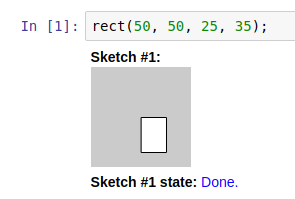
\includegraphics{images/processing.png}
\caption{Figure: a first sketch using Calysto Processing, a Java-based
language designed for creating art.}
\end{figure}

\textbf{Learning goals:} Reduce stress, build confidence, connect onto
their personal lives. Requires that they do learn the basics of Jupyter
including: log in, open a new notebook, enter the provided code, and
execute it. Often leads to a very animated, active learning classroom
activity (``How can I change the colors?'', ``How do I draw a circle?'',
etc.)

\textbf{Audience(s):} Beginning students.

\textbf{Format (lecture / lab / \ldots{}):} First day of class, in-class
exercise. Build on what students already know from typing and reading
(e.g., cut and paste, read top-to-bottom).

\textbf{Features:} Open ended, creative, fun.

\textbf{Pitfalls:} Works best when used with a pre-installed Jupyter
(see the \protect\hyperlink{jupyter}{relevant chapter}). Rather than
telling students that they can do it, just do it. As a first assignment,
to cut down on the vast possibilities, we suggest limiting the palette
of options. For example, restrict their drawings to use only a single
shape, such as rectangle or triangle. We suggest having the students
draw something in their life that is important or meaningful to them. We
suggest discussing the coordinate grid for the first assignment and
sketching an idea on paper first.

\section{Test driven development}\label{test-driven-development}

\textbf{Description:} The instructor provides tests written in a unit
testing framework like \texttt{unittest} or \texttt{doctest}; students
write code to make the tests pass.

\textbf{Example:} TODO: Necessary?

\textbf{Learning goals:} Helps students learn a good software
development process.

\textbf{Audience(s):} This pattern requires students to have some
programming experience.

\textbf{Format (lecture / lab / \ldots{}):} This pattern can be used for
in-class activities or homework.

\textbf{Features:} Helps students focus on the task at hand and know
when they are done (at least to the degree that the tests are complete).

\textbf{Pitfalls:} Some Python unit testing frameworks are not designed
to work with notebooks, and can be awkward to use. On the other hand,
\texttt{nbgrader} {[}TODO: add cross reference to nbgrader{]} supports
automated testing of the code students write in notebooks; in that
environment, the tests are not visible to students, which may or may not
be a bug.

This pattern required the overhead of teaching students about the unit
testing framework. Students working to make tests pass can lose their
view of the big picture, and feel like they have been robbed of
autonomy. This type of exercise is best used sparingly.

\section{Code reviews}\label{code-reviews}

Code reviews involve a student or instructor providing feedback on
someone else's code. This pattern involves peer work as well as a means
for providing feedback to students on topics other than correctness of
their code but also on code readability and styling.

\textbf{Example:} Present a problem to students that they must write a
solution to, say computing the square root of a number without using a
built-in function but have them write a test for their function that
uses a built-in function to compute the answer. After they are finished
have the students pair up and perform peer reviews of each other's code,
commenting not only on the way they solved the problem, such as making
up a list of pros and cons of their approaches, but also on the
readability of the code.

\textbf{Learning goals:} Learn to read and understand someone else's
code. Learn to write readable code.

\textbf{Audience(s):} Any group of students who are involved in coding.

\textbf{Format:} Once a suitable problem is formulated in a notebook (or
simply a script) then in-class review, as with the above example, can
work for peer reviews. Alternatively students can upload their
notebooks/scripts to a platform such as GitHub and the code reviews can
be done using the tools available there. Sufficient scaffolding must be
provided so that students understand the process, how to make
constructive comments and why the process is important. If an instructor
wants to review and provide feedback notebooks/scripts can be collected
and commented on with a similar explanation to students as to how they
are going to be graded (if they are).

\textbf{Features:} This pattern leads to not just feedback for the
person who wrote the code but also for the reader. Code review is also a
critical piece of the software development process used in industry
providing students with a view of the process. This can also have the
result of making sure that a student's code is readable via appropriate
code styling, commenting and documentation.

\textbf{Pitfalls:} Students need to be properly informed as to how the
code reviews will impact their grades, especially if peer review is
used. Notebooks on GitHub are not as easily reviewed as scripts.

\section{Bug hunt}\label{bug-hunt}

\textbf{Description:} The instructor provides a notebook with code that
contains deliberate bugs. The students are asked to find and fix the
bugs. Automated tests might be provided to help students know whether
some bugs remain unfixed.

\textbf{Example:} TODO

\textbf{Learning goals:} This pattern helps students develop programming
skills, especially debugging (of course); it also gives the practice
reading other people's code, which can be an opportunity to demonstrate
good practice, or warn against bad practice. It can also be used to
teach students how to use debugging tools.

\textbf{Audience(s):} This pattern requires students to have some
programming experience.

\textbf{Format (lecture / lab / \ldots{}):} This pattern can be used for
in-class activities or homework.

\textbf{Features:} Can be engaging and fun; develops important
meta-skills.

\textbf{Pitfalls:} The bugs need to be calibrated to the ability of the
students: if they are too easy, they are not engaging; if they are too
hard, they are likely to be frustrating.

\section{Adversarial programming}\label{adversarial-programming}

This pattern involves participants writing a solution to a problem and
tests that attempt to make the written solution fail. This pattern can
be done in many ways including having students complete the tasks and
pair up and exchange solutions/tests or having the instructor writing
the solution and the students then write the tests.

\textbf{Example:} Students are tasked to write a function that finds the
roots of a polynomial specified via some appropriate input. They are
also asked to write a set of tests that their function passes and fails
on. When students have completed these tasks they then exchange their
notebooks and use the tests they wrote on their peer's function. Finally
they will discuss any differences in their approaches and whether they
can come up with ways to not fail each other's tests or if the tests
provided are invalid.

\textbf{Learning goals:} Learn to write unit tests. Think critically on
how an adversary might break their solution.

\textbf{Audience(s):} Any group of students who are involved in coding.

\textbf{Format:} Decide on a sufficiently complex problem that may have
non-trivial tests written for it and write up the question in a
notebook. Then as an in-class activity or lab start the discussion
regarding the tests. If appropriate the instructor can collect notable
tests written by students and also share those.

\textbf{Features:} Provides a means for students to think critically
about a problem they are solving and how someone might break their
solution. Also can provide a learning activity with a form of
competition involved, which can then lead to an award system if desired.

\textbf{Pitfalls:} With competition come dangers if students are not
properly scaffolded so that they can provide constructive feedback. Some
problems and/or solution strategies are vulnerable to many corner cases,
leading to tedious whack-a-mole or fatalism that may distract from
learning objectives.

\hypertarget{jupyter}{\chapter{Jupyter Notebook
ecosystem}\label{jupyter}}

\section{Language support: kernels}\label{language-support-kernels}

The Jupyter system supports over 100 programming languages (called
``kernels'' in the Jupyter ecosystem) including Python, Java, R, Julia,
Matlab, Octave, Scheme, Processing, Scala, and many more. Out of the
box, Jupyter will only run the IPython kernel, but additional kernels
may be installed. Language support continues to be added by the open
source community and the best source for an up-to-date list is the wiki
page maintained by the project:
\url{https://github.com/jupyter/jupyter/wiki/Jupyter-kernels}. These
projects are developed and maintained by the open source community and
exist in various levels of support. Some kernels may be supported by a
vast number of active (and even paid) developers, while others may be a
single person's pet project. When trying out a new kernel, we suggest
exploring a kernel's community of users and documentation to see if it
has an appropriate level of support for your (and your students') use.

Jupyter's kernel flexibility allows instructors to pick the right
language for a particular context. For example instructors may use
Python to teach programming, while switching to R to teach statistics,
and then perhaps Scala to teach big-data processing. Regardless of the
language chosen, the Jupyter interface remains the same. Thus, some
cognitive load can be lessened when using multiple languages within or
across courses (e.g., the user interface stays the same between the
student's Digital Humanities and Biology courses). Students often
appreciate consistent use of the same language within a course, however.

\section{Using Jupyter notebooks}\label{using-jupyter-notebooks}

When using Jupyter notebooks on the data projector or large screen
monitor in the classroom, we recommend giving the students specific
instructions on the meaning of the user interface of the notebook. It is
not exactly intuitive.

The first and most salient component of the notebook is the \emph{cell}.
Indeed, the entire contents of a notebook is composed of only cells.
These cells can take one of two forms: text or code. We will descibe the
authoring of a notebook in the following section; however, here we
identify some of the subtle, yet important components of a code cell.

Code cells are composed of three areas: the \textbf{input} area, the
\textbf{display} area, and the \textbf{output} area. The input area is
identified by the \texttt{In\ {[}{]}:} prompt to the left of the cell.
Between the brackets of the \texttt{In} prompt can be one of three
items: a number, an asterisk, or a blank. A number indicates that this
cell has been executed and the value of the number indicates the order
of execution. For example, normally, after you execute the first cell
after opening a notebook, its prompt will read \texttt{In\ {[}1{]}:}.

\BeginKnitrBlock{rmdnote}
Pro Tip

When teaching with notebooks, you often will want to refer to a cell my
name. You could refer to a cell by its input prompt number. However,
keep in mind that this number will change if you excecute the cell
again, or that students may have different numbers if they, too, are
executing their own copy of the notebook. A better way of referring to a
cell may be to refer to the text right above the cell as that won't
change while you execute cells. For referring to lines of code, see the
following section on Tips and Tricks.
\EndKnitrBlock{rmdnote}

Before executing a cell, the input prompt number area will be blank.
Therefore, you can tell at a glance that that cell has not been executed
yet. It may also be the case that if an input prompt does have a number
in it, then the cell has been run in the past. However, the cell may not
have been run during this session, and thus the output may be showing
old results. We recommend running from the menu: \texttt{Cell},
\texttt{All\ outputs}, \texttt{Clear} at the beginning of a
presentation. That initializes all cell inputs to the blank state.

During the execution of a cell, the input prompt will contain an
asterisk. If it seems that too much time has passed and you still see
\texttt{In\ {[}*{]}:} your code may be in an infinite loop, or you have
lost communication with the kernel. You may have to interrupt or restart
the kernel. This is discuss below.

Finally, it is important to keep separate the display and output areas
below the input cell. The difference between these two areas is subtle
and confusing, but is very important in some instances. The display area
is reserved for any item that code has produced for viewing. That
includes simple text (i.e., \texttt{print("hello,\ world")}) or figures
from a plot. The output area is reserved for items that the cell
``returns.'' This is why in many notebooks you may see a variable
assignment followed immediately by the variable, like this:

\begin{Shaded}
\begin{Highlighting}[]
\NormalTok{x }\OperatorTok{=} \DecValTok{2434} \OperatorTok{+} \DecValTok{33476}
\NormalTok{x}
\end{Highlighting}
\end{Shaded}

In this example, you wouldn't actually see the value computed unless you
print it to the display area, or return the value. Here, we return it as
the last value of the cell.

\BeginKnitrBlock{rmdimportant}
Keep in mind that the bottom portion of the notebook on the screen or
monitor may not be visible to students in the back of the room. Make
sure that the font size is large enough, and that you don't go too fast
when demonstrating code that students don't have access to. We also
recommend that you hide the Jupyter toolbar and header to get more room
for the actual notebook (select \texttt{Toggle\ Header} and
\texttt{Toggle\ View} under the Jupyter \texttt{View} menu).
\EndKnitrBlock{rmdimportant}

\section{Authoring Jupyter notebooks}\label{authoring-jupyter-notebooks}

Before embarking on writing notebooks for your course, we recommend that
you look around on the internet for related courses. A similar course
for which an instructor has already generated notebooks could exist for
you to use or adapt for your course. Notebook authors often are happy to
collaborate on open source educational resources or have their resources
be used by other instructors. The following sections focus on Python
simply because it is currently the language with the largest Jupyter
feature support.

\subsection{Accessing documentation in the
notebook}\label{accessing-documentation-in-the-notebook}

One of the best features of quality libraries is their documentation,
which students and other users will likely consult regularly. From a
notebook cell, the TAB key autocompletes (or gives completion tips) and
SHIFT-TAB brings up full documentation. Similarly, using a question-mark
after a method or function will bring up the documentation after the
cell is run, as shown in Figure 5.1.

\begin{figure}
\centering
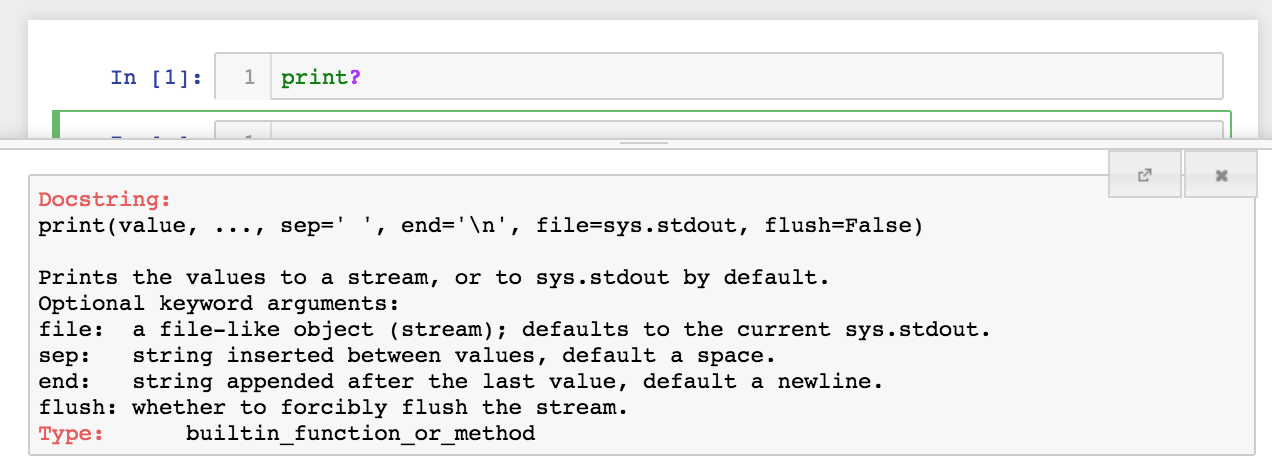
\includegraphics{images/chapter50.png}
\caption{A question mark used after a method or function brings up the
documentation after executing the cell.}
\end{figure}

Using this feature in class during live coding or while explaining how
code works helps make students comfortable of working effectively with
libraries.

\subsection{Widgets}\label{widgets}

Widgets provide the opportunity for learners and instructors to interact
with code outputs, such as charts and tables. Widgets are ``mini''
Graphical User Interfaces (GUI) that give the notebook user access to
slide bars, toggle buttons, and text-boxes. They can be used in
conjunction with code, allowing a change of mindset from programming as
a primary goal to exploring a model or computation as the primary goal.
Alternatively, the code can be hidden and the widgets used to create a
notebook ``app'' that might connect input parameters with a simulation
and a plot.

Currently, only a small subset of kernels have widget functionality. The
reference implementation of widgets are the Jupyter-Python widgets
(\url{https://ipywidgets.rtfd.io}). It includes widget components to
generate and display sliders, progress bars, text boxes, check boxes,
toggle buttons, etc. Many popular visualization tools, such as
Matplotlib, Plotly, leaflet.js, three.js, have Jupyter-Python widget
implementations. The documentation contains an up-to-date list of all of
the widgets and their variations. The \texttt{interact} method allows
you to wrap a function, which might be a simple computation or a complex
simulation that produces a plot, and provides widgets for each of the
inputs to the function. Figure 5.2 shows a simple example of a sinusoid
plot whose frequency is controlled by a slide-bar. Another kernel that
has some widget functionality is C++
(\url{https://github.com/QUantStack/xwidgets}).

\begin{figure}
\centering
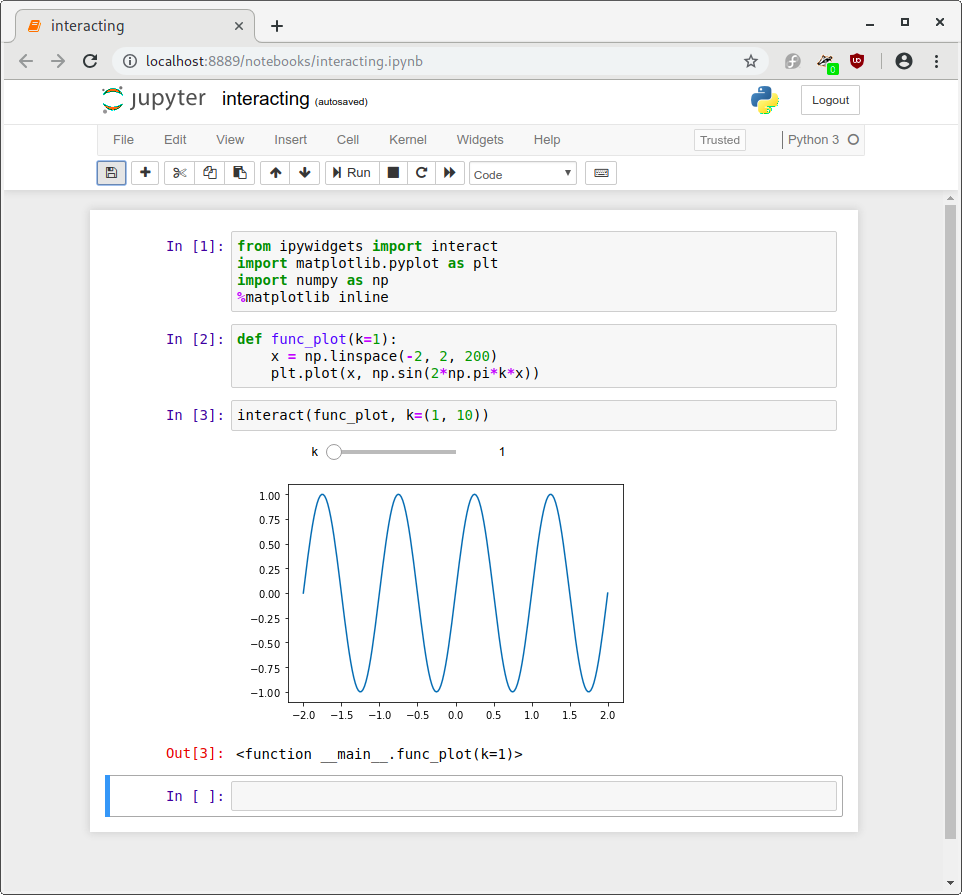
\includegraphics{images/notebook-matplotlib-interact.png}
\caption{Here, a slider allows the user to interactively change the
variable k in our function as we plot it.}
\end{figure}

In addition to the IPywidgets library, the ipyleaflet library
(\url{https://ipyleaflet.rtfd.io}) displays an interactive map in a
notebook.

\subsubsection*{Example}\label{example}
\addcontentsline{toc}{subsubsection}{Example}

\begin{verbatim}
from ipyleaflet import Map
Map(center=[34.6252978589571, -77.34580993652344], zoom=10)
\end{verbatim}

\begin{figure}
\centering
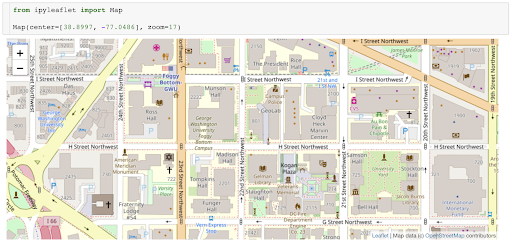
\includegraphics{images/chapter52.png}
\caption{Interactive map widget with \texttt{ipyleafletalt\_text}.}
\end{figure}

For the ambitions reader, there are resources available for you to write
your your own custom widgets. The widget cookie cutter project
(\url{https://ipywidgets.rtfd.io}) is a good place to start.

\subsection{Magics}\label{magics}

Magics are meta-commands that only function within Jupyter and allow a
user to access language/kernel-specific features. For instance, the
IPython kernel provides a number of magics that can be useful while
developing Jupyter notebooks using Python as the primary language. These
are
\href{https://ipython.readthedocs.io/en/stable/interactive/magics.html}{documented}
and we will only call out a few of these here. Many other magics are
available for different kernels but they are specific to Jupyter so may
not be usable in a stand-alone script in that language outside of
Jupyter. In some instances, you may want to use magics sparingly to
avoid obfuscating these meta-commands with the actual commands in the
language you are teaching. Magics always begin with either a single
\texttt{\%} for single-line commands or with \texttt{\%\%} for applying
a command to an entire cell. Some magics can be used with single or
double \texttt{\%}, but some cannot.

\subsubsection*{Examples}\label{examples}
\addcontentsline{toc}{subsubsection}{Examples}

\begin{itemize}
\item
  Matplotlib is a common choice for visualization. In Jupyter, the magic
  \texttt{\%matplotlib} allows the resulting figures to be displayed in
  the notebook: \texttt{\%matplotlib\ inline} produces static images
  embedded in the notebook, and \texttt{\%matplotlib\ \ notebook}
  produces interactive images (with zooming, panning, etc.).
\item
  The \texttt{\%run} magic allows running external scripts (and other
  notebooks), captures output and displays it in the notebook, e.g.,
  \texttt{\%run\ my\_script.py}. The \texttt{\%run} magic is one answer
  to ``how do I import one notebook into another?''
\item
  The \texttt{\%time} magic times the execution of the Python expression
  following it, e.g., \texttt{\%time\ sum(range(1000))}.
\item
  The \texttt{\%timeit} magic is similar to \texttt{\%time}, but it runs
  the expression multiple times and reports the average execution time.
\item
  The \texttt{\%reset} magic deletes all user-defined variables along
  with input and output. Magics often have ``flags,'' following the Unix
  command pattern. For example, \texttt{\%reset\ -s} is a soft reset and
  only removes user-defined variables. These commands can be useful to
  avoid problems with out-of-order execution problems.
\item
  The \texttt{\%debug} magic is used after code has stopped due to an
  exception (i.e., ``the program has crashed''). Enter the
  \texttt{\%debug} magic immediately after the crash, and you will be
  placed into the environment that caused the problem. From there you
  can explore variables and find the cause of the problem.
\end{itemize}

A good example of a magic operating on the entire contents of cell is
the \texttt{\%\%HTML} magic, forcing the cell to be interpreted as HTML
and rendered appropriately. You can also use magics to call other
languages while running the IPython kernel. For example, you can run R
code from within an IPython notebook by using the \texttt{\%\%R} magic.

\BeginKnitrBlock{rmdnote}
Pro Tip

In the IPython kernel you can also use the \texttt{\%shell} magic. This
is often abbreviated as \texttt{!} and can run and return results from
the shell/terminal. In IPython, you can also mix magics with regular
Python code. For example, \texttt{files\ =\ !\ ls} will use the
\texttt{ls} (list files) command in the terminal, return the list, and
set the Python variable \texttt{files} to that list.
\EndKnitrBlock{rmdnote}

\subsection{Notebooks under version
control}\label{notebooks-under-version-control}

Keeping notebooks under version control is a great way to not only keep
track of changes to your content, but also for sharing it. In a course
where multiple people are contributing to the development of notebooks
for the course, using version control in conjunction with a platform
like GitHub, allows authorship to be tracked and provides communication
tools for reviewing new contributions or outlining requested development
for a new assignment, activity, etc. Another advantage of using version
control is that some services will provide rendered views of notebooks
that you have made public. GitHub shows a rendered version of the
notebook, rather than the ASCII text that a notebook is comprised of.
Some pitfalls with LaTeX rendering may occur, as platforms do not always
render the notebooks the same as they would appear in an active Jupyter
interface.

We should mention a few caveats to keeping notebooks under version
control. The code output, including images, is stored in the repository,
unless you clear the output before committing changes. This can make
reviewing changes difficult, as changes in output will be detected even
when nothing has actually changed content-wise. The tracked notebooks
also can become large if output is tracked. Even when clearing the
output, reviewing changes can be awkward due to the format of the
notebook (notebooks are plain-text files and the file format is
represented as \href{https://www.json.org/}{JSON}). The community is
actively developing tools to make it easier to use version control with
Jupyter notebooks; one such tool is \texttt{nbdime} (see box).

\BeginKnitrBlock{rmdnote}
nbdime nbdime.readthedocs.io/

nbdime includes a set of tools for reviewing the changes (``diffs'') and
merging changes in Jupyter notebooks. You can compare versions of a
notebook using the terminal, view the changes richly rendered on a
browser, and merge in various ways. Because nbdime understands the
structure of notebook documents, it can make smart ``diffing and
merging'' decisions.
\EndKnitrBlock{rmdnote}

Another option to improve your version-control experience is to export a
Jupyter notebook to a markdown document, for example using the
\href{https://github.com/mwouts/jupytext}{jupytext} tool. Then you can
review diffs in the usual way for plain-text files.

\subsection{Testing notebooks}\label{testing-notebooks}

Before distributing notebooks, and in particular if you are working with
multiple contributors to the course material, testing the notebooks
before they are distributed to students or used in a live demo can help
mitigate unexpected bugs. At a minimum, you can test that the notebook
executes cleanly from top to bottom by restarting the kernel and running
all cells from top to bottom. This can be done from the menu (Restart +
Run all).

Though it requires a bit more setup, tests can be run automatically
using a continuous integration service, such as TravisCI
(\url{https://travis-ci.org}). This will require executing the entire
notebook via the command line, for example
\texttt{jupyter\ nbconvert\ -\/-ExecutePreprocessor.enabled=True\ -\/-to=html\ my\_notebook.ipynb}
will execute the notebook (same as pressing ``Restart + Run All'') and
then convert it to HTML. These services can be connected to GitHub so
that any time that the notebooks are changed, the tests are run
automatically. Simplifying this process is an area that is under
development in the open source community. The package
\url{https://github.com/opengeophysics/testipynb} provides an easy way
to test notebooks.

\subsection{Essential Python
libraries}\label{essential-python-libraries}

The purpose of this section is to introduce some of the most widely used
packages within the Python ecosystem. As mentioned before, over 100
kernels enable different programming languages in Jupyter. But Python is
a common choice in many disciplines, due to its large open-source
community which develops and maintains an ecosystem of over 150,000
software packages.

The core Python library
(\href{https://docs.python.org/3/}{https://docs.python.org}) contains
basic data types such as lists and dictionaries, as well as core
functionality such as arithmetic operators and simple file parsers. Most
tasks can be achieved with core Python. They are often made easier,
however, with higher-level libraries. This particularly applies for
scientific computing with Python. Among the vast number of packages in
the Python ecosystem, NumPy, Scipy, Matplotlib and Pandas are among the
most commonly used. A good resource for getting familiar with these
libraries is the \textbf{Scipy Lecture Notes}
\url{https://www.scipy-lectures.org}.

\begin{itemize}
\tightlist
\item
  Numpy (\url{http://www.numpy.org/}) is a fundamental library for
  numerical and scientific computing with Python. It contains data
  structures for numerical arrays, tools for linear algebra, random
  number capabilities, and much more.
\item
  SciPy (\href{https://docs.scipy.rg/}{https://docs.scipy.org/}) offers
  a varied set of functions for scientific computing, such as
  optimization, interpolation, statistics and signal processing. It also
  includes fundamental constants from many disciplines such as the speed
  of light as well as data structures for sparse matrices.
\item
  Matplotlib (\url{https://matplotlib.org/}) is the core plotting
  library for Python and can be used inline in the notebook with the
  \texttt{\%matplotlib\ notebook} or \texttt{\%matplotlib\ inline} cell
  magics.
\item
  Pandas (\url{https://pandas.pydata.org/}) provides resources for data
  analysis and a flexible data structures for labeled two-dimenstional
  data.
\end{itemize}

\subsection{Advanced topic: extensions}\label{advanced-topic-extensions}

There are many community contributed extensions that add functionality
to Jupyter notebooks. Extensions vary from displaying an automated table
of contents for a notebook, or prettify code, or hiding/showing solution
cells. Here is the link for how to install and enable extensions:
\url{https://jupyter-contrib-nbextensions.readthedocs.io/en/latest/install.html}

Here is a list of a collection of extensions that are bundled together:
\url{https://jupyter-contrib-nbextensions.readthedocs.io/en/latest/nbextensions.html}

Creating custom extensions is a way to extend or customize Jupyter to
add a capability that is not currently available with current extensions
or out of the box. These extensions may be targeted for a specific
kernel. Here are instructions for how to create and install custom
extensions:
\url{https://jupyter-notebook.readthedocs.io/en/stable/extending/frontend_extensions.html}

Figure X shows shows how Google Collaboratory, one of many tools to
interact with Jupyter notebooks, leverages the power of Jupyter
extensions for custom interaction and presentation.

\begin{figure}
\centering
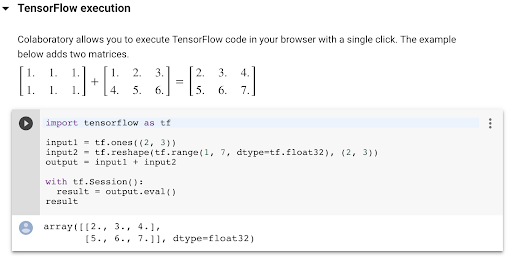
\includegraphics{images/chapter53.png}
\caption{Google Collaboratory uses Jupyter extensions to customize
Jupyter for their users. The run/play icon to the left of the code cell
is created using extensions. This is not present in the standard Jupyter
software. TensorFlow is a library for creating Machine Learning
experiments in Python.}
\end{figure}

The set of extensions for Jupyter is constantly evolving. Educators are
exploring new and interesting methods of using notebooks in pedagogy.
While the list of current extensions is far too long to list, you can
interactively experience some of the most useful extensions through this
live
\href{https://hub.mybinder.org/user/psychemedia-showntell-eii7j2nh/notebooks/index_computing.ipynb}{Binder
notebook} (Binder is described in detail in the following chapter). This
live notebook demonstrates the following:

\begin{itemize}
\tightlist
\item
  Turning on line numbers in code cells (makes it easier to refer to a
  line of code)
\item
  Code folding extension (hide code blocks to help focus attention)
\item
  Locked and frozen cells extension (prevent changes to cells)
\item
  An extension for a better user interface for error messages
\item
  A ``turtle'' extension (draws in a canvas in the notebook)
\item
  Block-based programming extension
\end{itemize}

The block-based programming extension (called Jigsaw) allows users to
program using drag-and-drop blocks of code that can be integrated with
other cells in a Jupyter Notebook (see figure). The advantages (and
disadvantages) of blocked-based languages are active research topics in
computer education research (see, for example, Mark Guzdial's excellent
\href{https://computinged.wordpress.com/}{Computing Education Research
Blog}, specifically
\href{https://computinged.wordpress.com/tag/blocks-based-language/}{those
posts on block-based languages}).

\begin{figure}
\centering
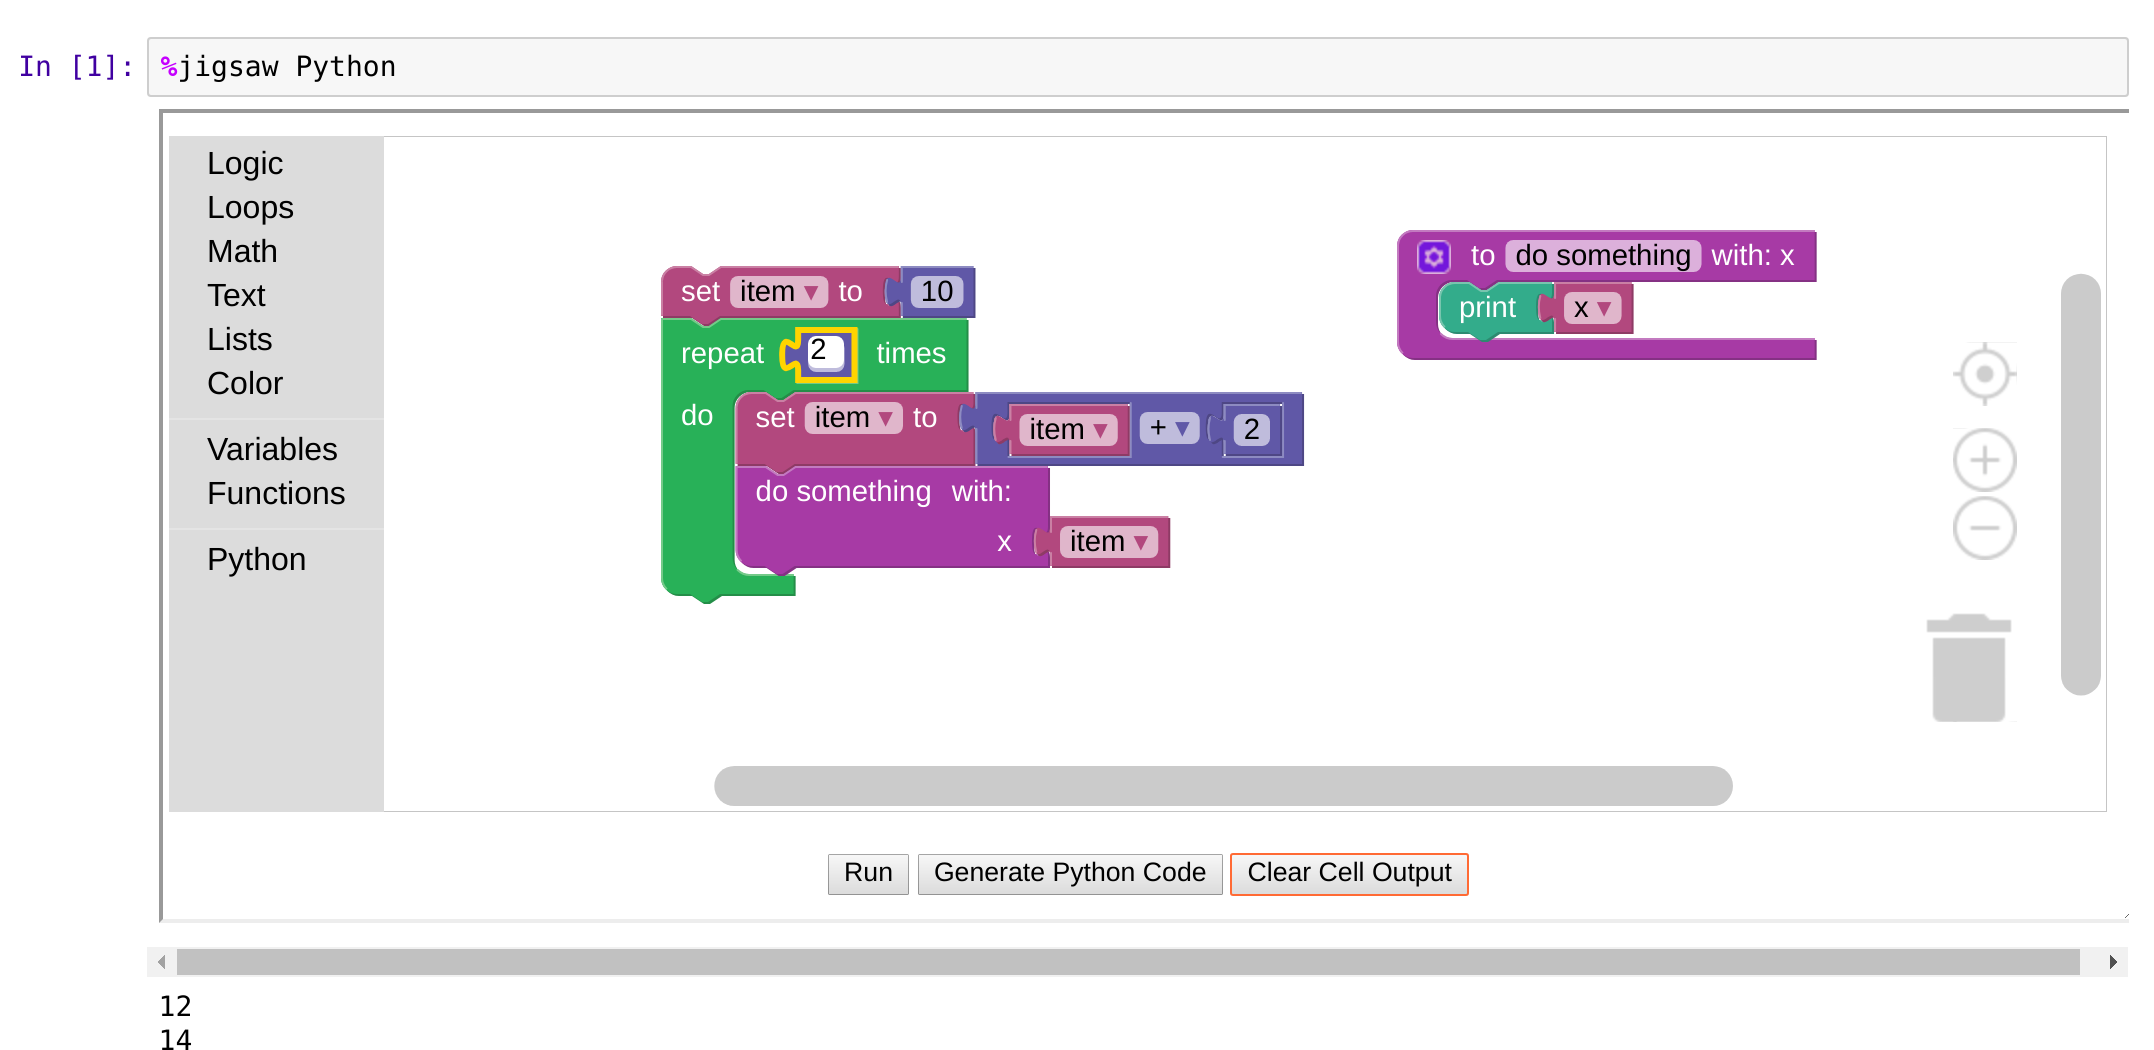
\includegraphics{images/jigsaw.png}
\caption{Example of incorporating Jigsaw, a block-based extension, in a
Jupyter Notebook. The extension allows the user to assemble code blocks
that can then be translated into Python or Java, and executed.}
\end{figure}

\section{Tips and tricks}\label{tips-and-tricks}

\subsection{Reminders}\label{reminders}

If you are using a single notebook as a standalone exercise in a
traditional class (i.e., this is the only computational component of
your class), then it is helpful to have a few cells at the top of that
notebook that reviews how to navigate through the notebook and how to
insert cells, etc.

\subsection{Feedback}\label{feedback}

How do we get feedback from students in an interactive session to see if
students have completed an exercise?

A low tech solution is to give students sticky notes of different
colors, one meaning ``finished'' and one meaning ``need help'', that
they can stick on the back of their computers. The instructor can then
quickly look up to take a survey of the state of the class and decide
how to proceed.

Projecting Slack or a similar chat group on a screen and having student
copy-paste solutions (provided they are short functions) is a nice way
to let everyone in the class see one another's solutions. A positive
aspect of having multiple student solutions projected is that it can
show the variety of ways to solve a problem. This gives an opportunity
to talk about the readability of solutions and their efficiency. A
downside is that in a large class, the shear volume of posts can make it
overwhelming. Instead polling can be used to aggregate student answers
and provide some form of feedback to the instructor. Nbgrader or
travis-CI can also be options here, requiring students to submit
completed code where it is assessed automatically. These will however
require more setup and can take some time to complete.

\subsection{Explaining each cell}\label{explaining-each-cell}

Consider moving the comments for a code block into a markdown cell
either directly above or below the code cell. Comments in a markdown
cell often read much better and give you more flexibility in discussing
or describing the code. However, short comments in a block of code can
still be useful.

\subsection{How to structure code
cells}\label{how-to-structure-code-cells}

How much code should you put in a cell? You will develop your own style
of writing noteooks with experience. Typically, you will want to keep
the number of lines low so that it is easy to follow, and you can have
useful comments above the cell. However, we recommend putting code that
``goes together as a meaningful unit'' into a single cell. For example,
if you have lines of code that are highly dependent on each other, then
you might want to put them together. As an example, consider two lines
of code: one that opens a file, and the second that reads the data from
the file. It is probably a good idea to put those into the same cell so
that they are always executed together. Otherwise, the student may
encounter errors if they execute cells independently a second time
(e.g., there are no more data).

Specifically, messing up the dependencies between cells is where most of
the confusion using notebooks comes from with new users. For example, if
you change a variable's name (without restarting the notebook), then the
following code cells may continue to use the old variable's name (and
value). Later, when running the notebook again, the notebook may fail in
unexpected ways because the old variable no longer exists. This is
sometimes referred to as ``the hidden state problem.'' This is an open
research problem, and researchers are exploring various possible
solutions. For example, trying searching the internet for ``jupyter
dependency graph'' or ``jupyter dataflow notebook.''

\BeginKnitrBlock{rmdnote}
Pro Tip

You can easily split a cell into two parts at the cursor using the
keystroke \texttt{CONTROL} + \texttt{SHIFT} + \texttt{-}. You can also
merge multiple cells with \texttt{SHIFT} + \texttt{m}. Both of these are
also available from the menu under \texttt{Edit}.
\EndKnitrBlock{rmdnote}

On the other hand, it is often a useful idea to separate lines of code
where you want to provide the student a place to interactively add
cells, and examine the state at that particular point in the process.
Asking probing questions in a Socratic method is a very useful technique
for engaging the reader and encouraging them to become more than a
reader. Students do not naturally know to insert cells and explore items
in a notebook. You will need to explicitly teach this skill. In fact,
teaching students how to effectively weave code into their \emph{own}
notebook stories is an important component of teaching with notebooks.

\subsection{Custom styling}\label{custom-styling}

New notebook creators often try to centrally manage the formatting of
headings, equations, and other textual items. For example, rather than
using a standard markdown heading, a creator may over-design the
headings by using HTML styles. This may create two problems:

\begin{enumerate}
\def\labelenumi{\arabic{enumi}.}
\item
  The rendering of the notebook markdown may change and your formatted
  HTML header may not maintain the same look over time.
\item
  Headers created using markdown can be used by notebook tools, such as
  automatically creating a Table of Contents.
\end{enumerate}

Our recommendation is to resist the desire to customize the styling and
simply use the default representations. If you want to do customization
(for example if you want to color certain cells) you can use CSS.

\subsection{Length of notebooks}\label{length-of-notebooks}

Notebook authors sometimes make the notebooks very long with many topics
and sections. Notebook sections and cells are currently not easily
reused in a copy/paste sense for mixing intra-notebook content. Until
this functionality is available, we recommend that authors make short,
self-contained notebooks around short topics. This allows other
notebooks authors to mix and match notebooks to create curriculum.

\section{Gotchas}\label{gotchas}

\subsection{\texorpdfstring{Programming language \(\neq\)
Jupyter}{Programming language \textbackslash{}neq Jupyter}}\label{programming-language-neq-jupyter}

Teaching a class entirely with Jupyter can give the sense to students
that this is the way all computational exploration is done. In
particular, students can be confused into thinking that programming
requires the notebook, instead of understanding that a notebook is just
one way to interact with a particular language. This point should be
made clear periodically. A good way to reinforce this is to show how to
take a function that has been developed and debugged in a notebook and
cut-paste it into a script (such as a file ending in .py for Python) and
then import it into the notebook to regain that functionality. Also, the
Integrated Development Environment (IDE), Spyder, has a plugin
(\url{https://github.com/spyder-ide/spyder-notebook}) that allows
notebooks to be displayed alongside Python scripts and a python terminal
which can be useful for showing this dichotomy.

\begin{figure}
\centering
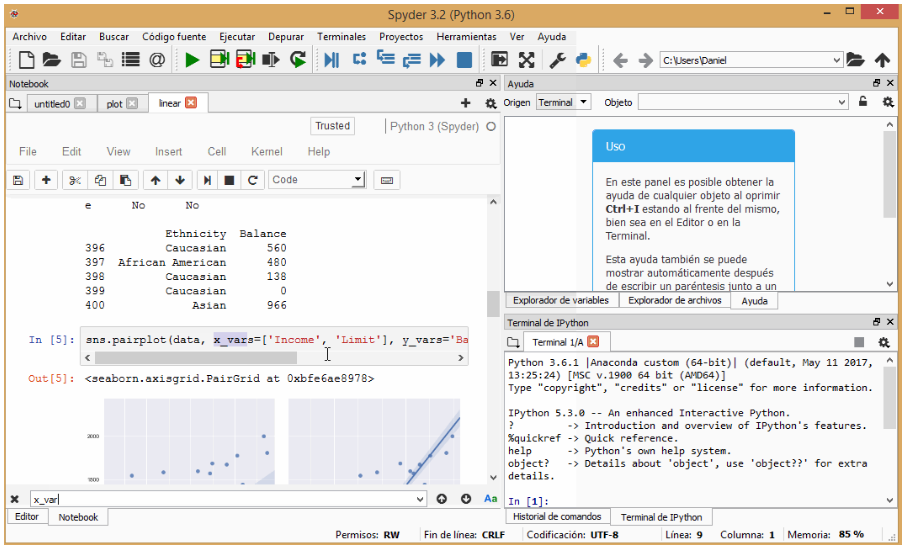
\includegraphics{images/chapter54.png}
\caption{Jupyter notebook displayed in a window pane inside Spyder.}
\end{figure}

\subsection{Restart, restart,
restart\ldots{}}\label{restart-restart-restart}

Often, students may need to stop a computation, and this can be
accomplished by pressing the ``Interrupt'' button in the toolbar.
However, students should also be made aware of how to restart the kernel
in a notebook, and what this means. There are several instances when
students might need to do this. Sometimes students write code that can
go into an infinite loop. The visual cues that notebooks give in this
case are subtle, and students may not realize this and don't understand
why the notebook is non-responsive. In live-coding situations, it can be
useful to demonstrate this to students and show them how to restart the
kernel and carry on.

A second instance of where restarting a kernel might be needed is due to
how the notebook stores the state of the computation. We like to think
that, since the notebook is laid out in a linear fashion, that the state
will always reflect what would happen if the notebook was run from the
start up to that point. However, it is common to work in a notebook out
of order, for instance if students ask a question about some previous
example. If the variable has been changed in subsequent cells, then its
value might not reflect what you expect when you rerun a cell earlier in
the notebook. Restarting the kernel is sometimes the only solution.

\subsection{Notebook hygiene}\label{notebook-hygiene}

Many gotchas can be mitigated by developing notebooks that will be
robust to incremental and non-linear execution. The main principle is to
minimize side-effects of executing a cell and manifests itself somewhat
differently in different languages; our suggestions here will be
relevant to Python and may need to be adapted for other languages.
Notebooks should generally be able to execute sequentially, such as via
``restart kernel and run all cells''. (An exception is when a notebook
is intentionally incomplete for the purpose of live coding or student
exercises, see nbgrader or the exercise estnations for more elegant ways
to handle this.) Variable mutation is the most common way in which a
notebook may malfunction when executing cells in a non-linear way (e.g.,
in response to student questions or when comparing and contrasting
different methodologies). Sometimes this mutation is incidental, through
dummy variables that were not meant to have significance outside the
scope of the cell in which they are used. Their scope can be limited by
placing them in a function, even if that function is only called once.
Redefinition of functions can often be avoided by parameterizing the
desired functionality as would typically be done if designing a library
(though this may be a distracting software design for novice
programmers). Function definitions should have little or no dependency
on variables from their enclosing scope. When modifying cells for demos
and formative assessments during class, it is useful to either copy the
cell or modify/execute such that a conforming implementation remains
present when moving on to other cells where it may be used.
Additionally, you can minimize these issues by grouping code in a single
cell that should always be executed sequentially, because code within a
cell will always be sequential.

\chapter{Getting your class going with Jupyter}\label{getting-going}

You have several options on how to get Jupyter notebooks to your
students. You can ask students to install Jupyter on their own
computers, install Jupyter on lab computers for students to use, or run
Jupyter on a remote server that your students access on the internet.

\section{Local installation on students' or lab
computers}\label{local-installation-on-students-or-lab-computers}

``Local installation'' means that each computer is running the software
that includes the Jupyter Notebook. Typically, this requires installing
a distribution that includes Jupyter, Python, and possibly other
language kernels.

A popular software distribution that includes Jupyter is Anaconda, which
is easy to install on Windows, Mac, and Linux. Because it can install
everything with user level permissions, it does not require the user to
have administrator (or root) access to the computer. Anaconda includes
over 1500 software packages providing most, if not all, needed software
for learners. Jupyter notebooks can be opened by launching Jupyter or by
opening them through the Spyder IDE. These attributes make it attractive
for both personal use and for installation on institution controlled
computers.

\BeginKnitrBlock{rmdnote}
What is Anaconda?

You will see the Anaconda distribution recommended by many educators and
course authors. Anaconda is a package manager, an environment manager, a
Python distribution, a collection of over 1,500+ open source packages,
including Jupyter. It is free to download, open source, and easy to
install, on any computer system (Windows, Mac OS X or Linux). It also
includes the conda packaging utility to update and install new packages
of the Python and R ecosystems, and to manage computational
environments. According to the company's webpage, Anaconda has more than
6 million users; see: What is Anaconda?. The Software Carpentry project
provides installation instructions for Anaconda, with videos.
\EndKnitrBlock{rmdnote}

Two other easily installable software packages that can run Jupyter
notebooks are \href{https://nteract.io/}{nteract} and
\href{https://nteract.io/atom}{Hydrogen}. nteract is installed by
downloading a binary installer from their website and double-clicking
the installation file. nteract's simple user interface make it an
excellent choice for students new to computer programming. Once nteract
is installed, any Jupyter notebook on a student's local system with a
graphical interface can be double-clicked and it will open within
nteract. Hydrogen is a \href{https://atom.io/packages/hydrogen}{very
popular plugin} for the open source Atom editor; it's currently used by
over 700,000 people. Hydrogen lets a user edit, display, and execute a
notebook within the Atom editor.

You can ask students to install Jupyter on their own computer or make it
possible for them to use it on lab computers. These can also be
combined: give students the instructions to install it on their own, but
also tell them that it's available in the lab if they can't get it to
work on their laptop. This way you don't need a large enough computer
lab for everyone, and don't need to worry that not everyone can get it
to work on their own.

\subsection{Jupyter on student-owned
computers}\label{jupyter-on-student-owned-computers}

The benefits of installation on student-owned computers include:

\begin{itemize}
\item
  Once students have the software on their computers, they always have
  access to it; they can work anywhere, and they can use it for
  internships, jobs, and other non-school activities.
\item
  It is easy for them to install additional packages later.
\item
  Students learn to install and set up Jupyter, and software in general,
  which is a skill they are likely to need.
\item
  The total computing power for the class scales with the number of
  students, as long as each student has enough CPU power and memory to
  support the intended applications.
\item
  You can adopt Jupyter without support or resources from your
  institution.
\item
  Students learn to use Jupyter on their preferred OS, e.g.~Linux, Mac,
  or Windows, which means they are already familiar with the basic
  idioms of their OS.
\end{itemize}

Drawbacks include:

\begin{itemize}
\item
  This approach is only possible if every student owns a computer with
  enough capacity.
\item
  Students with less powerful computers might be at an unfair
  disadvantage.
\item
  Although installation is generally easy, it still takes time. The time
  you spend at the beginning of a class can be worthwhile for a
  semester-long course that uses Jupyter throughout, but it is a barrier
  to using Jupyter for a single module or one-off assignment in a course
  about something else.
\item
  Also, the amount of time spent debugging esoteric problems scales with
  the number of students: a class of 25 students is bound to have a few
  people with 32-bit processors, incompatible libraries, out-of-date
  operating systems, over-zealous virus checkers, etc., and a class with
  100 students will have four times as many. One work-around is to have
  students work in pairs: the probability that more than half of the
  students cannot get it working is reduced.
\item
  Discrepancies in installed library versions can cause issues for
  students and may lead to different behaviors when students run code.
\end{itemize}

Although Jupyter is cross-platform and ideally behaves the same on
Windows, Mac, or Linux, and distributions such as Anaconda also behave
very similarly on all platforms, the instructions for installing and
launching it are slightly different on each operating system, so
fine-grained instructions such as ``double click here'' or ``type this
command'' need different versions for Linux, Mac, and Windows users,
which can be challenging when the instructor presenting the material has
only one platform at their disposal. It is worth developing detailed
instructions that the students can go through at their own pace, rather
than relying only on a live demo in class that will only apply to a
fraction of the students.

\subsection{Jupyter on lab computers}\label{jupyter-on-lab-computers}

Using lab computers instead of student-owned computers has the benefits
of uniformity and improved equity. Each student will have exactly the
same setup, and the instructions will work the same for everyone. This
reduces the amount of individual tech support required and guarantees
that all students have access to enough computational power.

However, this deployment has some disadvantages:

\begin{itemize}
\item
  Depending on how much control you have of the computer lab, you might
  need institutional permission and support.
\item
  Students might be limited to working on assignments only when they are
  on campus and when computer labs are open, which might be an unfair
  disadvantage for non-resident students or those with full time jobs.
\item
  It might be difficult to install additional packages as the need
  arises, and students might not be allowed to install packages they
  need for projects.
\item
  Even in a computer lab, it can be difficult to maintain consistency
  across machines, and to keep all installations functional.
\end{itemize}

\section{Jupyter on remote servers}\label{jupyter-on-remote-servers}

Even when Jupyter runs locally, it runs as a web application; that is,
it runs in a browser connected to a server. In a local installation, the
browser and the server run on the same machine. But it is also possible
to run the server remotely.

In that case, students don't have to install anything; they only have to
run a browser and load a URL.

There are several ways to run Jupyter on a remote server:

\begin{enumerate}
\def\labelenumi{\arabic{enumi}.}
\tightlist
\item
  You can run Jupyter on a server owned by you or your institution.
\item
  You can run Jupyter in a temporary environment running in the cloud.
\item
  You can run Jupyter in a persistent environment running in the cloud.
\end{enumerate}

Running Jupyter remotely has many of the advantages of running in a lab:
you can provide a consistent environment and guarantee that all students
have access to sufficient computation resources. And it mitigates one of
the drawbacks of a lab installation, since students have access to cloud
resources from anywhere, not just on campus.

Working in the cloud also means that students do not have to manage
their own backups of a laptop hard drive. Although a student could still
inadvertently overwrite, delete, or destroy the contents of a notebook
stored in the cloud, they will not lose their entire work if a laptop is
damaged or lost.

For simple, one-off uses of Jupyter (say, for a single assignment or
in-class activity) the cloud option is very attractive as it requires
little in-class time to discuss installation of additional software.

\subsection{Running in a temporary environment in the
cloud}\label{running-in-a-temporary-environment-in-the-cloud}

The easiest option for running Jupyter in the cloud is to use a cloud
service that provides temporary environments. Some of these services are
free of cost, and you can use them without installing anything.

These environments are well-suited for short examples in classes that do
not use Jupyter extensively. Students can open a notebook and start
running with the push of a button.

However, there are some limitations to these services:

\begin{itemize}
\item
  If your notebooks depend on particular packages, or particular
  versions of packages, it can be difficult to satisfy these
  requirements.
\item
  These services run notebooks in a temporary environment that
  disappears if it is left idle. So they might not be suitable for
  managing student work.
\item
  Some of these services do not guarantee a level of service and may not
  be as reliable as you need for a class or workshop.
\end{itemize}

\BeginKnitrBlock{rmdnote}
Binder mybinder.org

Binder is an open-source service provided by Project Jupyter. It allows
the owner of a set of notebooks residing in a public repository to
pre-build an image in the Binder service, and get a shareable link that
any visitor can use to obtain a working instance of JupyterHub,
pre-loaded with the notebooks in the repository. The session is
temporary (any changes the user makes will be deleted when closing the
tab or window), but it's fully interactive. Binder is currently one of
the favorite services for running one-off workshops or tutorials.
\EndKnitrBlock{rmdnote}

\subsection{Running on servers you
control}\label{running-on-servers-you-control}

If you have access to a server or cluster with enough computing power to
support your class---including CPU and especially memory---you can
provide a Jupyter as a service using JupyterHub.

JupyterHub is open-source software that provides a cloud-based Jupyter
application for each user in a group. Each user has their own account
and home directory on the server. The Hub, JupyterHub's central system,
allows authenticating users and starting individual Jupyter notebook
servers. Programs that start notebook servers can use a variety of
technical solutions. For more details, see
\url{https://github.com/jupyterhub/jupyterhub/wiki/Spawners}

Once the Hub starts a user's notebook server, the Jupyter Notebook
running in the cloud behaves just like Jupyter does when installed on an
individual's computer, but JupyterHub will be running notebooks and
storing files on a remote cloud computer. Students can download
notebooks stored in the cloud to their local computer if they wish to
work with a local installation as well. Additionally, students can
upload notebooks (and other files) from their local computer to the
cloud.

While anyone can run a JupyterHub server on their own Linux or Mac
computer, installing and configuring JupyterHub requires sophisticated
knowledge spanning the Linux/Unix operating system, system
administration, and networking. For more information, see:

\begin{itemize}
\item
  \url{https://github.com/jupyterhub/jupyterhub} (the basic JupyterHub
  project, which can be installed on a bare-metal server, a virtual
  private server (VPS), or a commercial cloud cluster)
\item
  \url{https://github.com/jupyterhub/the-littlest-jupyterhub} (a
  simplified installation of JupyterHub on a remote server or VPS)
\item
  \url{https://github.com/jupyterhub/zero-to-jupyterhub-k8s} (a
  step-by-step guide to install JupyterHub on a Kubernetes cloud system)
\end{itemize}

Providing a JupyterHub service offers several benefits. First, students
get up and running immediately---they spend no time installing software.
They navigate to a web URL, log in to JupyterHub, and begin using
Jupyter. This ability to quickly log in and begin computing is a
powerful way to get students to engage with the lesson, builds
confidence, and avoids the sometimes-stressful experience of installing
software on the student's computer.

However, running JupyterHub on your own server has drawbacks:

\begin{itemize}
\item
  Getting started is not easy; most instructors would require (or at
  least benefit from) institutional support that may not be available.
\item
  It can be difficult to scale: if the number of students increases, you
  might need more computing power. And the load students generate can be
  uneven; for example, if everyone runs a computationally-intensive
  example at the same time, your server might not be able to handle it.
\item
  This option can be expensive, unless you already have servers with
  sufficient power.
\end{itemize}

\subsection{Running Jupyter in the
cloud}\label{running-jupyter-in-the-cloud}

If you or your institution don't own computing hardware with the power
to support your class, you can run JupyterHub on virtual servers
provided by cloud services like AWS and Microsoft Azure. In those
environment, you can install JupyterHub as described in the previous
section

Commercial offerings also exist to use Jupyter in the cloud, some of
which provide free trials or a ``freemium'' pricing model. They include:

\begin{itemize}
\item
  CoCalc (previously SageMathCloud) (\url{https://cocalc.com}) is an
  online \href{https://github.com/sagemathinc/}{open source} computing
  environment with
  \href{https://cocalc.com/doc/jupyter-notebook.html}{first class
  support for Jupyter notebooks} supported by SageMath, Inc. It is one
  of the few services that allows multiple users to edit a Jupyter
  notebook simultaneously. It also allows the notebook user to cycle
  through the revision history of a notebook and provides a number of
  popular kernels by default. The service includes the ability to share
  files with project collaborators. It is free to use and greater
  computational resources can be obtained by paying the monthly, yearly,
  or course based subscription fees. Instructors can pay for resources
  for an entire class or ask students to pay and subscribe for a
  semester. Instructors can make use of the
  \href{https://tutorial.cocalc.com/}{course management system} for
  assignment distribution, collection, grading, and more. The free
  version limits access to the internet to prevent abuse, effectively
  blocking use of standard package managers. While an instructor could
  work around this limitation by uploading files to the service or
  requesting the company to install software, this is likley onerous for
  many users. Paid versions lift this limitation and allow use of
  \href{https://github.com/sagemathinc/cocalc/wiki/How-to-Install-Python-Packages-into-CoCalc}{standard
  package managers (e.g.~pip, conda, R, Julia, etc)}.
\item
  Gryd (\url{https://gryd.us}) is another subscription service with a
  free tier. It includes course-management features, like a way to
  create a course, invite students, and deploy auto-graded assignments.
\item
  HubHero (\url{https://hubhero.net}) provides professionally configured
  JupyterHub servers for teachers. For courses of up to about 30
  students they offer \href{https://hubhero.net/community/}{the
  community install} which gets you your own JupyterHub on your own
  hardware or a cloud provider of your choice. For larger courses or
  fully managed deployments \href{https://hubhero.net/hosted/}{hosted
  solutions} are available as well. Hub Hero is owned by
  \href{https://github.com/betatim/}{Tim Head} a project lead for
  \url{https://mybinder.org} and contributor to JupyterHub.
\item
  codio (\url{https://codio.com/features/ide})
\item
  Microsoft Azure notebooks (\url{https://notebooks.azure.com/} )
\item
  Amazon Sagemaker
  (\url{https://docs.aws.amazon.com/sagemaker/latest/dg/ex1-prepare.html})
\item
  Gradient by Paperspace (\url{https://www.paperspace.com/gradient})
\item
  Google Colaboratory (\url{https://colab.research.google.com/} )
\end{itemize}

The biggest advantage of these services is that they require no
installation and minimal setup by instructors, and some of them provide
features that integrate with learning management systems. However,
instructors generally have to create student accounts and set up student
environments.

These services are highly scalable; that is, they can handle large
numbers of students and uneven loads. However, they are not infallible;
they might require some tending to make sure students have access to
enough resources.

The biggest drawback of these services is that they can be expensive.
Some charge on a per-student basis, with limits on computation and
memory use. Some charge on the basis of actual use, which can be
unpredictable (and might require instructors to enforce limits on
student activities).

Other drawbacks include:

\begin{itemize}
\item
  It may be difficult or impossible to install packages you, or
  particular versions of packages.
\item
  Some of these services impose limits on what students can do; for
  example, they might have limited ability to access external services.
\item
  Many of these services are relatively new, and they sometimes expose
  instructors and students to rough edges.
\item
  Students generally lose access to their accounts when the class ends
  (or a limited time after).
\item
  There may be privacy concerns with sharing student information on
  commercial servers. Some institutions have agreements with one or more
  of these providers that address privacy.
\end{itemize}

\section{Distribution and collection of
materials}\label{distribution-and-collection-of-materials}

You may want to distribute course materials to and collect them from
students. A variety of options are available. Some important things to
consider:

\begin{itemize}
\item
  Do you want to share your notebooks publicly, or do they require
  privacy?
\item
  Can the notebooks that the students create or edit be public? Or do
  they require privacy?
\item
  How do you plan to assess collected notebooks?
\item
  Do you need integration with your LMS?
\item
  Do you need integration with a file-sharing system?
\item
  Do you want to distribute with the cell output showing?
\item
  Do students need software that is not easily available on their own
  (or laboratory) computers?
\end{itemize}

Jupyter notebooks are plain text computer files, so you can distribute
them to students and collect them using any system that handles text
files, including GitHub, Google Drive, and (as a last resort) email
attachment.

\subsection{Learning management
systems}\label{learning-management-systems}

Many instructors use a Learning Management System (LMS) to communicate
with students. These tools offer private file sharing and assignments
that connect to the students' institutional computing accounts and they
can be used to distribute and collect notebooks as text files. However,
most LMS tools are not yet notebook-aware, so they don't render
notebooks or make it easy for instructors to comment on or grade them.

Some tools and workflows are being actively developed to connect the
Jupyter ecosystem to the LMS ecosystem using the
\href{https://open.edx.org/learning-tools-interoperability}{Learning
Tools Interoperability (LTI)} standard. By the time you read this, you
might find that the options have improved.

\subsection{Web hosting}\label{web-hosting}

Notebooks can be publicly hosted on any website, so students can
download the files by clicking on a link. Most web-hosting software is
not notebook-aware, but you can use \texttt{nbviewer} to share public
notebooks, rendered as a static web page.

\BeginKnitrBlock{rmdnote}
nbviewer nbviewer.jupyter.org

nbviewer is a web service provided by Project Jupyter. You can enter the
URL of any publicly hosted notebook, and get a web page with the content
of the notebook fully rendered. Some browser extensions and add-ons let
you open a notebook in nbviewer with a button click. See: Open in
nbviewer.
\EndKnitrBlock{rmdnote}

\subsection{GitHub}\label{github}

One of the popular tools for distributing and collecting notebooks is
GitHub, a hosting and collaboration platform for software. GitHub is
based on git, a \emph{version-control system}. Files under version
control are often hosted on services like GitHub, GitLab, or Bitbucket,
all of which are notebook-aware. For example, when you view a notebook
on GitHub, you see a rendered notebook that includes formatted text,
typeset mathematics, code highlighting, and the output of the code,
including figures.

GitHub Pages (and other similar services) can also be used to host
rendered notebooks, and continuous integration services can build the
web pages from the notebooks and then display the content. See: Jupyter
Book and use of \href{https://drdoctr.github.io/doctr}{\texttt{doctr}}
to do this.

Educators at academic institutions can use GitHub Classroom, which
allows instructors to set up assignments for a class. Students click on
a link for an assignment and a copy of the assignment repository is
created and initialized with the assignment content, which can be a
notebook. Each student's repository can be made private, with access
only granted for the student and instructor. This can be an efficient
way to distribute assignments to a large class.

A drawback of git is that it is hard to use. It might be worth spending
time in your class to teach git, if it is valuable for students to learn
about version control. But if this is not one of the learning goals for
your class, you can minimize the students' exposure to git using
graphical interfaces like GitHub Desktop and git for Windows.

The default git tools for comparing files and merging changes do not
work well with Jupyter notebooks. However, some specialized tools can
help with these tasks (see Notebooks Under Version Control).

\subsection{JupyterHub}\label{jupyterhub}

If your students are using JupyterHub, you can place notebooks and any
related files directly into the students' directories manually or via a
script. If \texttt{nbgrader} is available on your JupyterHub instance
you can use it to collect and distribute notebooks (whether or not you
choose to use \texttt{nbgrader}'s assessment features). This allows you
to develop the notebooks and incrementally make them visible to the
students for them to ``fetch''. They can then edit the notebooks or
create new ones in the directory created in their storage space, and
then publish their notebooks back to you for downloading, viewing, or
assessing with the \texttt{nbgrader} tools (see the next section for
details on this tool).

\BeginKnitrBlock{rmdnote}
nbgrader

nbgrader is a tool for creating, handling, and automatically grading
assignments based on Jupyter notebooks. It works as a Jupyter extension
that the course creator installs on their computer. nbgrader is a
flexible project in the Jupyter ecosystem that allows the distribution
and collection of materials. As its name implies, it also can grade
assignments; it can be used in a distributed manner where each student
is running Jupyter on their own computers, or in a centralized manner,
for example, if the students each have an account on a JupyterHub
installation. (More details in the Assessment section.)
\url{https://nbgrader.readthedocs.io}
\EndKnitrBlock{rmdnote}

\subsection{\texorpdfstring{Using an LMS and \texttt{nbgrader}
together:}{Using an LMS and nbgrader together:}}\label{using-an-lms-and-nbgrader-together}

Integration of \texttt{nbgrader} with learning management systems is
still primitive, but the following is a strategy that works with current
tools.

\begin{enumerate}
\def\labelenumi{\arabic{enumi}.}
\item
  The instructor creates an assignment notebook using \texttt{nbgrader},
  then distributes the assignment to students via an LMS.
\item
  Students complete the assignment and upload the solution to the LMS.
\item
  The instructor downloads the completed assignments as a zip file and
  extracts the students' solutions in a Jupyter environment.
\item
  Instructors and graders use \texttt{nbgrader} to grade the assignment
  and save the grades to a CSV file.
\item
  The CSV file is then uploaded to the LMS.
\end{enumerate}

Some tools that make this workflow easier include the Extractor plugin
to the
\href{https://nbgrader.readthedocs.io/en/stable/plugins/zipcollect-plugin.html}{ZipCollect}
feature in \texttt{nbgrader}.

\section{Assessing student learning with Jupyter
notebooks}\label{assessing-student-learning-with-jupyter-notebooks}

Many educators develop course-assessment activities as Jupyter
notebooks. This includes exams, in-class activities, homework
assignments, and projects.

Simple ways to handle the assessment of a notebook-based submission:
have students either print them out, email them, submit them as a
standard electronic document (say, into the LMS), or drop them into a
shared folder. At that point, the instructor can mark and grade them in
a traditional manner, for example by writing comments on a printout or
adding annotations to a PDF.

\BeginKnitrBlock{rmdnote}
Pro Tip

Printing out a notebook can sometimes result in wasted space on pages,
especially for notebooks with many images or figures. Converting to PDF
requires large/complex LaTeX installations. Exporting to HTML and then
printing often gives a better result.
\EndKnitrBlock{rmdnote}

\texttt{nbgrader} allows code cells in a notebook to be marked to be
auto-graded or manually graded. An instructor can then create an
assignment that can be completely auto-graded, requiring little work
after the notebook has been created. This makes grading much easier and
scales well with large class sizes. However, creating such an
auto-graded notebook in \texttt{nbgrader} can be quite time-consuming.
In addition, pedagogically a completely auto-graded notebook may have
serious downsides. For example, studies suggest that students learn
better when they can actively connect a topic to their own interests
{[}CITATION NEEDED{]}. One method of encouraging this is to have a
``reflection'' question on each submission. Such a reflection question
can encourage students to comment on the material in a personal way, but
it cannot be auto-graded. Another downside is that simply autograding
code with unit tests is unlikely to assess many of the learning
objectives you might have for an assignment, e.g., ability to use
specific software-design patterns. To address this, you can create
manually graded cells for a portion of an assignment and provide written
feedback to the student.

\BeginKnitrBlock{rmdnote}
Caution

At the time of this writing, nbgrader has some limitations that require
careful use. For example, using it in a multi-class setting (say, on
JupyterHub) requires that instructors coordinate the naming of
assignments so that they do not collide.
\EndKnitrBlock{rmdnote}

\texttt{nbgrader} is a sophisticated tool that can be set up to allow
multiple graders, teaching assistants, and more. For more information on
using \texttt{nbgrader}, see \url{https://github.com/jupyter/nbgrader}.

Some third-party notebook-based assessment solutions do exist. For
example \href{www.cocalc.com}{CoCalc},
\href{www.vocareum.com}{Vocareum}, and \href{https://gryd.us}{Gryd}
provide a cloud notebook platform that can also grade assessments
similar to or using nbgrader.

{[}TODO{]} \_For example, cocalc.com offers\ldots{} {[}are there other
third-party course management notebook-oriented solutions?{]} and
Berkeley uses DataHub for their large Data8 course. Vocareum
(\url{https://www.vocareum.com}) TODO

\section{How do you create Jupyter notebooks for reuse and
sharing?}\label{how-do-you-create-jupyter-notebooks-for-reuse-and-sharing}

As you create notebooks for your lectures, computational essays, or
homework assignments, you may wish to think about how to make it
possible that they can be reused by yourself and others.

First, you may want to make the materials openly accessible and findable
via the internet. This suggests avoiding keeping the notebooks behind a
``walled garden,'' such as a Course Management System. That is, users
may have access to some material, but be prevented from seeing other
materials. You will have to decide whether you want others to have full
access. For example, many teachers do not want students to be able to
see notebooks that may have solutions, or hints of solutions and
therefore limit their access.

\begin{quote}
To share your notebook with others you can submit it to
\url{https://www.engage-csedu.org/}. This curated collection of open
educational computing resources is maintained by the
\href{https://www.ncwit.org/}{National Center for Women in Information
Technology (NCWIT)}.
\end{quote}

If you decide to make your notebooks reusable by others, make it clear
under which license the materials can be used. For example, you can
include a
\href{https://creativecommons.org/licenses/by-sa/3.0/us/}{Creative
Commons attribution and share-alike} statement at the bottom of your
notebook. Adding a license allows people to reuse your materials without
asking for permission explicitly.

GitHub may be the most common service to host and share notebooks, where
they can be viewed (including rendering), downloaded, or forked by
others. (Private repositories can also be used to limit visibility to
colleagues, students, or other organizations.). Make sure to be aware of
some of the pitfalls of keeping notebooks version controlled however
(see Notebooks Under Version Control for details).

Another potential issue with sharing deals with external files that you
may want to include in your notebook. This is in contrast with content
(say a plot) that can be directly created by the notebook's code.
Possible content includes data, images and videos using code and
embedding tags in markdown or HTML. The implication is that if you share
your notebook you must include the external files along with the
notebook. This can be done a number of ways including using a version
control repository, a zip-file, or a file sharing service. Another
external dependency issue with sharing notebooks involves software
libraries. In this case you share a configuration file that a user can
use to setup the same environment. Examples of these files include a
conda \texttt{env.yml}, a pip \texttt{requirements.txt}, or
\texttt{dockerfile}.

Because Jupyter notebooks embed the output of cells into the ipynb file
itself (e.g., images, videos, etc.), the files can grow large. To make
it possible to display the cell output via the renderers on Github,
Gitlab, or nbviewer, save the notebook after it is executed and then
upload to those services. If instead you want to reduce file size and
provide the notebooks to someone with the code cell output cleared,
choose this option in the notebook's dropdown interface. Then the user
will need to execute the notebook themselves to see the output.

\section{Jupyter: a 21st Century genre of Open Educational Resources and
practices}\label{jupyter-a-21st-century-genre-of-open-educational-resources-and-practices}

Educators create teaching and learning materials. With the appearance of
the internet, a community of educators began producing open access
traditional teaching materials. In parallel, a community of software
developers began creating open source software. Each community developed
their own development patterns. In particular open source software
communities gravitated to the bazaar style\footnote{The bazaar style is
  a method of collectively creating software that isn't top down
  directed like a traditional company hierarchy.} of distributed and
collaborative work. Jupyter notebooks may be the first time that these
communities are merging. Jupyter notebook authors are applying the
content creation patterns they use to the creation of open educational
resources that teach computation or teach through computation.

Open Education encompasses a large community, with its own conferences
and journals, with leaders and advocated practices. The most visible
efforts are related to Open Educational Resources (OER): the creation
and adoption of openly licensed learning materials. In 1994, Wayne
Hodgins coined the term ``learning object'' and the idea spread that
digital materials could be designed and made to be \emph{reused}. This
was followed by efforts to develop metadata standards, content
exchanges, and so on (addressing the concern of how to find the objects
to reuse them). In 1998, David Wiley coined the term ``open content''
and spread the idea that principles of Free and Open Source Software
(FOSS) could be applied to content on the World Wide Web (OpenContent,
\protect\hyperlink{ref-OC1998}{1998}). The Creative Commons non-profit
organization was founded in 2001 to provide ready-made license
agreements for sharing content and served a vital infrastructure role on
the spread of OER. The Creative Commons licenses are now the most widely
used licensing framework for open education. The year 2001 also saw the
launch of MIT OpenCourseWare (OCW). MIT promised free public access for
non-commercial uses of their course materials. It was a unique
commitment at an institutional level, strengthened by the MIT brand.
Other universities joined the OCW movement: Rice with the OpenStax
project (now formerly Connexion), CMU with the Open Learning Initiative
(OLI), Utah State University with the Center for Open and Sustainable
Learning, and so on. Today, the Open Education Consortium has hundreds
of members from around the world. The recurrent topics in OER are:
reducing costs for students buying textbooks, increasing access, and
dealing with copyright and licenses.

In the last few years, educators using Jupyter have been creating and
sharing all kinds of educational materials in the form of notebooks,
typically under a Creative Commons Attribution license (CC-BY). In fact,
Jupyter is \emph{a new genre of OER}. But in addition to creating open
content, educators using Jupyter often take active part in the Jupyter
community and adopt the \emph{culture} of open-source software. This is
a culture with strong ethical commitments, related to freedom of access,
transparency, and governance (Coleman,
\protect\hyperlink{ref-coleman2012coding}{2012}). The content they
create has the value of giving access (the very definition of OER),
under an open model. But open-source culture also promotes a culture of
collaboration. In this regard, engaging in teaching with Jupyter opens
new possibilities for educators to engage in \emph{open development} and
collaborate with others in producing lessons, tutorials, courses, and
even books.

\chapter{Usage case studies}\label{case-studies}

Contributors to this chapter: you may increase adoption by new users if
you integrate information about some of the following into your case:

\begin{enumerate}
\def\labelenumi{\arabic{enumi}.}
\tightlist
\item
  Demonstrate that you can increase students' ability to:

  \begin{enumerate}
  \def\labelenumii{\arabic{enumii}.}
  \tightlist
  \item
    Engage material \& participate in class
  \item
    Understand material and perform well
  \item
    prep their for career
  \item
    Enjoy learning this way
  \end{enumerate}
\item
  describe:

  \begin{enumerate}
  \def\labelenumii{\arabic{enumii}.}
  \tightlist
  \item
    how it fits with how their students learn
  \item
    how it connects to how they teach
  \item
    the needed resources (support, hardware, etc.)
  \item
    the necessary logistics (e.g., how much time will it take? Be
    honest: time is a consideration, and an important reason that people
    do not adopt new practices, but is not a reason that they stopped
    using one)
  \item
    what Jupyter does in terms of promoting learning, instructor
    affordances
  \end{enumerate}
\end{enumerate}

\section{Jupyter notebooks in support of scaling for large
enrollments}\label{jupyter-notebooks-in-support-of-scaling-for-large-enrollments}

\subsection{Supporting large enrollment courses at UC
Berkeley}\label{supporting-large-enrollment-courses-at-uc-berkeley}

The University of California at Berkeley started a pilot course titled
``Foundations in Data Science'' (also known as Data-8) for about 100
incoming undergraduate students in Fall 2015. Data-8, the fastest
growing course in Berkeley's history, is entirely Jupyter-based,
allowing the program to scale the course to 1,400 students in 2018. This
scale is made possible by Jupyter's shared computational environment. In
particular, Jupyter allowed ``browser-based computation, avoiding the
need for students to install software, transfer files, or update
libraries'' (see The Course of the Future and the Technology Behind It
{[}\url{https://data.berkeley.edu/news/coursefuture}{]}). Data-8 is
powered by JupyterHub and all the course materials are published openly
(\url{http://data8.org}).

\subsection{Large-scale adoption: Jupyter across
Canada}\label{large-scale-adoption-jupyter-across-canada}

Recognizing the importance of data science, computational research, and
educational resources, the \href{https://www.pims.math.ca/}{Pacific
Institute for the Mathematical Sciences (PIMS)}, in partnership with
\href{https://www.computecanada.ca/}{Compute Canada} and
\href{https://www.cybera.ca/}{Cybera}, have launched JupyterHub
platforms (under the project name Syzygy) to support researchers and
educators across Canada. Syzygy (\url{http://syzygy.ca}) provides access
to cloud-hosted Jupyter resources using existing institutional
credentials and encourages the development of computational and data
science skills. It is currently accessible at 16 institutions across the
country (McMaster, Queen's, SFU, UAlberta, UBC, UCalgary, ULethbridge,
UNewBrunswick, UOttawa, URegina, USask, UToronto, UVic, UWashington
(US), UWaterloo, Yorku) and has been used by over 11,000 people at those
institutions.

Syzygy is extensively used for teaching, but is also being used for
research activities. One notable example is a scientific software
seminar at the University of British Columbia, where graduate students
and post-doctoral researchers meet to share and learn data science
techniques with their peers. Initiatives are also underway, as part of
syzygy, to deepen its relevance into research by providing seamless
access to larger and more varied types of resources (GPUs, parallel
machines, different language kernels etc.).

Callysto (\url{https://callysto.ca/}) is a related project, also
launched by PIMS and Cybera, to bring Jupyter to students in Canadian
middle and high schools (grades 5-12). Callysto focuses on creating and
curating open content (\url{https://github.com/callysto}). This content
forms the basis of project workshops, where teachers can work through
the materials interactively, before taking them back to their
classrooms. The content links to a supporting JupyterHub installation
(integrated with the authentication systems for the networks of school
districts) allowing easy access to the materials and a Jupyter
environment to learn and create in.

-- Ian Allison

\subsection{Quick switch: moving an existing course to Python and
Jupyter (at the last
minute)}\label{quick-switch-moving-an-existing-course-to-python-and-jupyter-at-the-last-minute}

For many years, our chemical engineering kinetics course had used
software for differential equation and nonlinear simultaneous equation
solving to simulate reactors and solve design problems. The software,
recommended and described by the textbook, was installed in the
college's computer labs, but licenses for student-owned computers were
expensive and it was only available for Windows. In Spring 2015, I was
informed my class now had 52 students, but the largest computer lab had
room for only 40. As the semester progressed and we neared the chapters
that required numerical simulation, I rewrote the examples using Python
and SciPy and created Jupyter notebooks, walking students through the
steps involved in setting up and solving the problems. I found Lorena
Barba's open-source MOOC materials online, and adapted these for my
``getting started'' notebooks. I had students install Anaconda on their
own computers, and got everyone up and running without any central
infrastructure or support from the college's IT staff. I found the
Jupyter Notebook format of including ``lecture note'' style commentary
along with short, unintimidating, snippets of code, to be extremely
effective. A couple of years later I passed on the course to a new
instructor, who took my course materials, taught himself some Python,
and continued to use Jupyter notebooks for content delivery and
assignments.

The first year was a bit rough around the edges as I introduced it quite
late in the semester. Still, it is clear that the approach resonated
with students. An alumnus from my 2016 course wrote, ``I thought that
your course was very successful, especially the use of Jupyter Notebook
as a classroom and assignment tool. I still remember specific problems
that we went over in class (e.g., the microfluidic reactor array with
heterogeneous catalysis), and I feel that the use of Python to solve
problems throughout the course greatly benefited my understanding of
fundamental concepts. I went on to use Python {[}in the pharmaceutical
industry{]}, where I built tools for bioinformatics data analysis,
mutation network profiling for protein engineering experiments, and RNA
structure prediction from experimental data and molecular
thermodynamics.''

-- Richard West

\section{\texorpdfstring{The ``CFD Python'' story: guiding learners at
their own
pace}{The CFD Python story: guiding learners at their own pace}}\label{the-cfd-python-story-guiding-learners-at-their-own-pace}

``CFD Python'' is a collection of Jupyter notebooks based on a practical
module that I began using in class in my Computational Fluid Dynamics
(CFD) course at Boston University in 2009. The 5-week module develops
worked examples that build on each other to incrementally guide the
learner to create a program to solve the Navier-Stokes equations of
fluid mechanics, in 12 steps. In 2013, I was invited to teach a
mini-course in the Latin-American School in High-Performance Computing,
in Argentina. The Jupyter notebooks platform allowed me to create a
guided narrative to support learners with different background
experience and knowledge. For that event, we wrote notebooks based on
the CFD course module, to use as instructional scaffolding in the
2-full-days of minicourse. Twenty students worked through the notebooks
as self-paced lessons, while I went from desk to desk asking and
answering questions. About four of the students completed all the
lessons in the 2 days, a bulk of them achieved up to about Step 8, and a
few of them lagged behind in Steps 4 or 5 by the end of the course. For
those who completed the full module, they had achieved in 2 days what my
regular students in the classroom normally took 5 weeks to do. Seeing
that was an eye-opening moment: both the power of worked examples in
code, and the ability to allow learners to follow their own pace made a
remarkable difference in these learners.

\emph{REF --- Barba, Lorena A., and Forsyth, Gilbert F. (2018). CFD
Python: the 12 steps to Navier--Stokes equations. Journal of Open Source
Education, 1(9), 21, \url{https://doi.org/10.21105/jose.0002} }

Based on the experience developing the ``CFD Python'' learning module,
we adopted this basic design pattern for creating lessons using
computable content:

\begin{enumerate}
\def\labelenumi{\arabic{enumi}.}
\tightlist
\item
  Break it down into small steps
\item
  Chunk small steps into bigger steps
\item
  Add narrative and connect
\item
  Link out to documentation
\item
  Interleave easy exercises
\item
  Spice with challenge questions/tasks
\item
  Publish openly online
\end{enumerate}

-- Lorena A. Barba

\section{Analyzing music with
music21}\label{analyzing-music-with-music21}

I became interested in learning more about Python in 2013 after reading
a tutorial by Luciano Ramalho as he was writing Fluent Python. Since I
tend to seek out projects that match my outside interests (music, art,
and nature) I was looking for Python projects with music and came across
Myke Cuthbert's music21 project. Music21, an open source music theory
and analysis library maintained by Professor Michael Cuthbert at MIT,
provides a set of tools to answer questions about music quickly and
simply. Users can create, analyze, and share music with just a few lines
of code. Myke's use of the notebook hooked me. Unlike many things that I
had worked on before, the notebooks made it easy to get started and to
write small code snippets that did real work! The more I used the
notebooks and showed them to people that I taught at Fab Lab San Diego,
the more that I saw the power of the notebook to engage a user and
empower them to explore and learn.

Music, a universal language, appeals to learners of all origins, ages,
education levels, and interests. As a subject that casts a wide appeal,
music offers the opportunity to engage and delight learners. It's an
accessible subject that has a low barrier to entry for learners from
disciplines beyond computer science and engineering.

-- Carol Willing

\textbf{Education benefits}

\begin{itemize}
\tightlist
\item
  lessons notebooks can be tailored to age appropriate content within
  music
\item
  multisensory
\item
  ability in K12 to align with the standards
\item
  possibilities for bringing in multi-subject learning

  \begin{itemize}
  \tightlist
  \item
    writing
  \item
    history
  \item
    math
  \item
    science
  \end{itemize}
\item
  accessibility through audio and braille
\end{itemize}

\textbf{Misc quotes (perhaps pick a couple?):}

\emph{``I think of music21 as being composed of two parts. The first is
infrastructure, routines for reading, writing, and manipulating musical
scores, while the second consists of a higher-level analytical
toolkit---generating a Roman numeral from a chord and key, putting
chords into normal form, checking for parallel fifths, identifying
scales containing a given pitch or chord, and so on.'' ---Bruce
Tymoczko, Professor of Music, Princeton}

Inclusive

\emph{``It's not exclusive, but inclusive, which is the whole spirit of
jazz.'' --- Herbie Hancock}

Education

\emph{``So, you can't stay in one place, no matter how comfortable that
place is. It's all about growing.''---Mavis Staples}

Universal

\emph{``Music in the soul can be heard by the universe.''---Lao Tzu}

Communication

\_Music is the greatest communication in the world. Even if people don't
understand the language that you're singing in, they still know good
music when they hear it.``---Lou Rawls\_

\emph{``In the beginner's mind there are many possibilities. In the
expert's mind there are few.'' --Shunryu Suzuki}

\section{Interactivity in computer science (high school and middle
school)}\label{interactivity-in-computer-science-high-school-and-middle-school}

\textbf{Who}

High school and middle school students at Cal Poly SLO's EPIC program
completed a two hour workshop on Interactivity in Computer Science. The
workshop participants included dual language learners (English as a
Second Language) and students who have had limited access to computers
prior to the workshop.

\textbf{Why}

Providing early access to at-risk groups who may not see themselves as
capable of learning to code or use computation

Illustrate that there are many skills beyond math and science that are
needed to create software applications

\textbf{What}

Two hour workshop that maximizes ``hands on'' exploration with the goal
of building an ongoing interest in computer science

\begin{itemize}
\tightlist
\item
  short lectures
\item
  interactive discussion - LISTEN
\item
  hands on - DO/APPLY This section is self-paced to engage different
  learning styles and prior knowledge
\item
  recap - DISCUSS
\item
  8 or so projects with achievements outlined
\item
  modern curriculum including p5.js, jupyter, binder, deep learning and
  machine learning with TensorFlow and Magenta (art and music)
\item
  Goal is to empower students to understand that they CAN use CS to
  solve real world problems
\end{itemize}

Instructor Approach

\begin{itemize}
\tightlist
\item
  Start with high quality engaging content
\item
  Self contained notebooks
\item
  Use widgets to add additional interactivity
\end{itemize}

\section{Interactive geophysics with
Jupyter}\label{interactive-geophysics-with-jupyter}

The GeoSci.xyz project (\url{https://geosci.xyz}) is an effort to
develop a community of scientists and educators around learning
resources and software for the geosciences. The project includes
multiple open-source textbooks, each which have associated Jupyter
notebook ``apps'' that serve as interactive simulation engines for
exploring concepts in geophysics. We have used these resources in an
undergraduate course on applied geophysics at the University of British
Columbia; this course is primarily taken by by geologists and engineers
(non-geophysics majors). In 2017, we delivered a 2 day short course for
professionals, graduate students, and researchers in 26 different
countries around the world (\url{https://disc2017.geosci.xyz}). In both
of these courses, the goal is to provide learners with an overview of
the various geophysical methods (e.g.~magnetics, gravity, seismic,
electromagnetics) and concepts governing the physics; we do not dive
into details of the math nor do we expect students to program or write
any lines of code. The role of Jupyter notebooks in these courses is to
serve as a tool for visualizing and exploring the physics.

During a lecture, the notebooks as a presentation medium lend to a
dynamic presentation style, where we as instructors can select model
parameters based on student input. Concepts are reinforced as students
then use these same notebooks in labs and assignments. We have found
that the notebook apps are most effective when students are first asked
to critically think about what they expect to see and then visualize the
result. If the resultant image matches their expectation, then they
understand the concept, and if not, it is an opportunity to learn and
further explore.

-- Lindsey Heagy

\begin{figure}
\centering
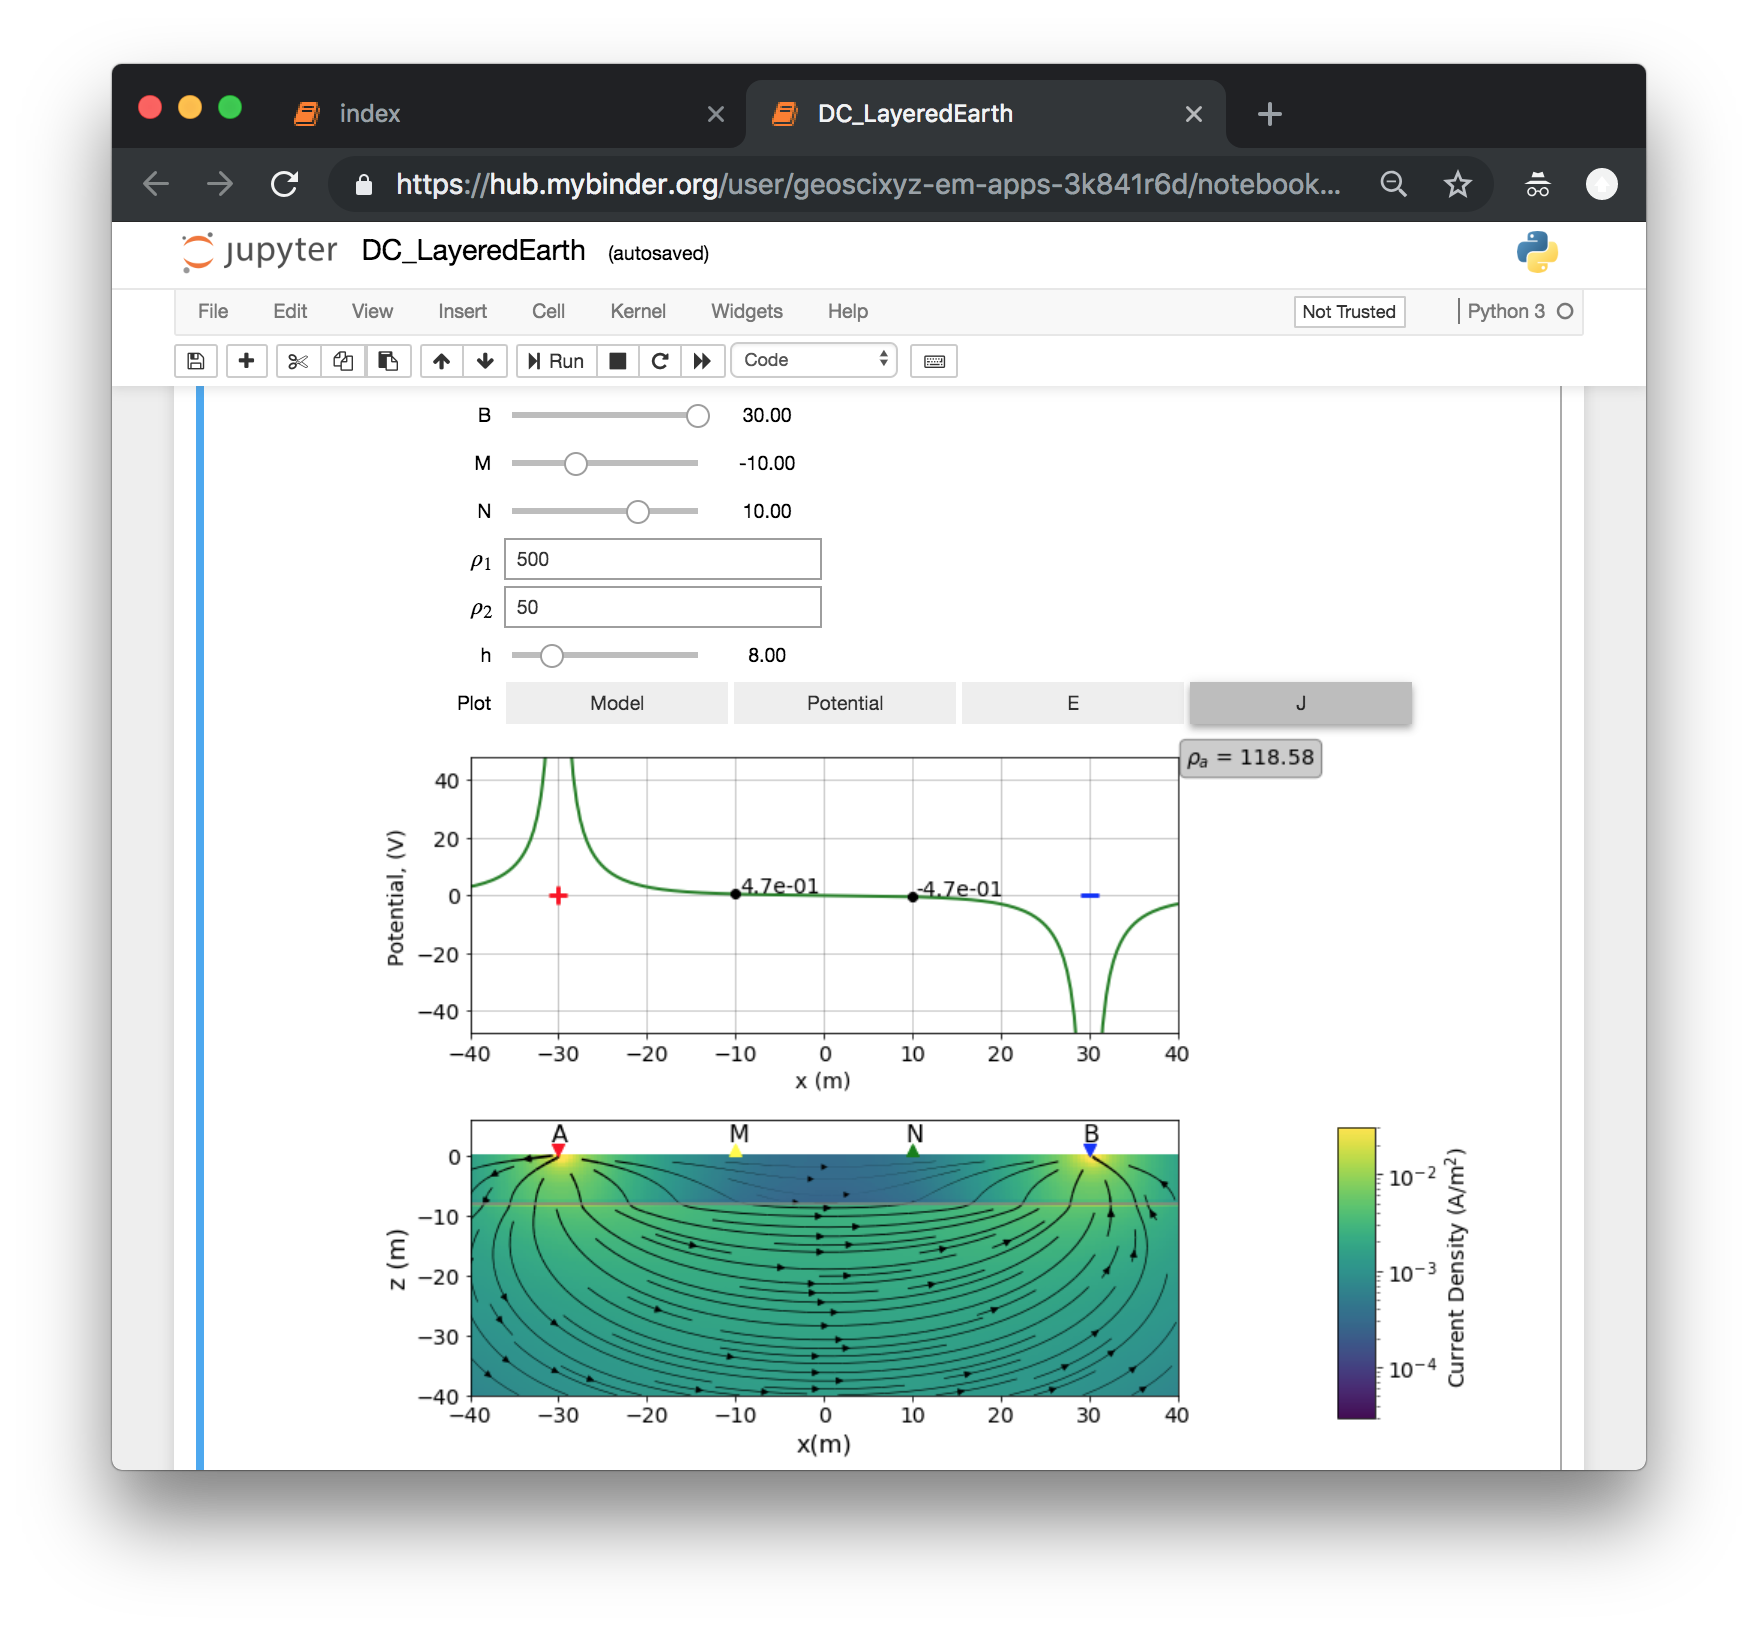
\includegraphics{images/DC-layered-earth-app.png}
\caption{Notebook ``app'' for exploring the direct current resistivity
experiment over a two layer earth
(\url{https://em.geosci.xyz/apps.html}).}
\end{figure}

\section{Investigating hurricanes}\label{investigating-hurricanes}

\textbf{Who}

Middle school and high school students visiting Columbia's School of
Engineering and Applied Sciences on a field trip

\textbf{Why}

Students often come through looking to tour labs and experience some of
the research that is being done at the school. Unfortunately certain
fields, in this case computational mathematics and hurricane research,
do not lend themselves to these types of events.

\textbf{What}

Instead of a lab or lecture a computer lab was reserved for an hour and
a Jupyter notebook used to walk students through some basic
visualizations and data analysis encouraging students to change the code
displayed to answer questions such as ``Where did Hurricane Sandy go?''
and ``What storms occurred during 1981?''. This includes a number of
visualizations of hurricane tracks, coloring by strength of storms, and
an analysis of average number of storms per year. Notebook is available
at \url{https://github.com/applied-math/demos}.

-- Kyle T. Mandli

\begin{figure}
\centering
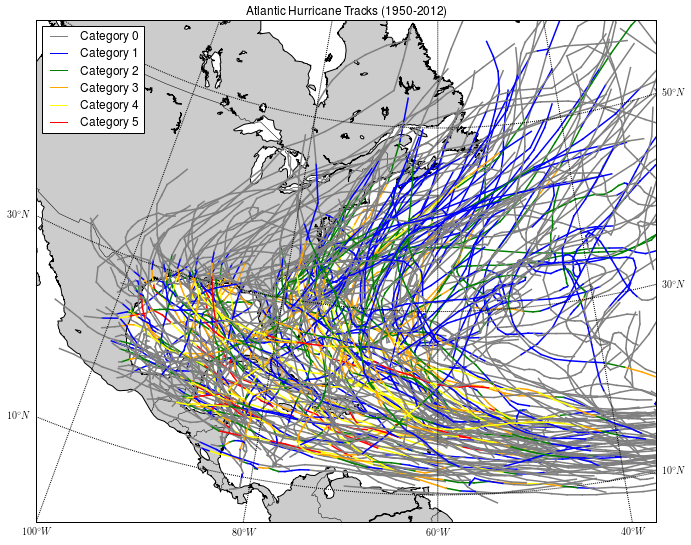
\includegraphics{images/hurricanes.png}
\caption{Visualization from the notebook at
\url{https://github.com/applied-math/demos} demonstrating the paths of
Atlantic hurricane tracks from 1950-2012 with coloring demonstrating
category of storm.}
\end{figure}

\hypertarget{authors}{\chapter{About the authors}\label{authors}}

\section{Project lead}\label{project-lead}

\subsection*{Lorena A. Barba}\label{lorena-a.-barba}
\addcontentsline{toc}{subsection}{Lorena A. Barba}

\begin{itemize}
\tightlist
\item
  George Washington University
\item
  \href{mailto:labarba@email.gwu.edu}{\nolinkurl{labarba@email.gwu.edu}}
\item
  \href{https://twitter.com/LorenaABarba}{@LorenaABarba}
\end{itemize}

Lorena A. Barba is Associate Professor of Mechanical and Aerospace
Engineering at the George Washington University. She adopted Jupyter in
2013 and since then used it in every course she teaches. Her open course
materials are well known and used by thousands of learners:
\href{http://lorenabarba.com/blog/cfd-python-12-steps-to-navier-stokes/}{CFD
Python} and
\href{https://github.com/numerical-mooc/numerical-mooc}{Numerical MOOC}
are the best examples.

\section{Authors at the sprint}\label{authors-at-the-sprint}

\subsection*{Lecia J. Barker}\label{lecia-j.-barker}
\addcontentsline{toc}{subsection}{Lecia J. Barker}

\begin{itemize}
\tightlist
\item
  University of Colorado Boulder
\item
  \href{mailto:lecia.barker@colorado.edu}{\nolinkurl{lecia.barker@colorado.edu}}
\item
  \href{https://twitter.com/leciab}{@leciab}
\end{itemize}

\href{https://www.colorado.edu/cmci/people/information-science/lecia-barker}{Lecia
Barker} is an Associate Professor and Associate Chair of Undergraduate
Studies in the
\href{https://www.colorado.edu/cmci/infoscience}{Department of
Information Science} at the University of Colorado Boulder. She is also
a Senior Research Scientist for the
\href{https://www.ncwit.org/}{National Center for Women \& IT}. Her
research group is studying the
\href{https://csteachingpractices.wordpress.com/}{diffusion and adoption
of teaching practices} in undergraduate computer science. Lecia holds a
Ph.D.~in Communication from CU Boulder and an MBA in Marketing from San
Diego State University.

\subsection*{Douglas Blank}\label{douglas-blank}
\addcontentsline{toc}{subsection}{Douglas Blank}

\begin{itemize}
\tightlist
\item
  Bryn Mawr College
\item
  \href{mailto:dblank@brynmawr.edu}{\nolinkurl{dblank@brynmawr.edu}}
\item
  \href{https://twitter.com/dougblank}{@dougblank}
\end{itemize}

\href{https://cs.brynmawr.edu/~dblank/}{Douglas Blank} is Associate
Professor in the \href{https://cs.brynmawr.edu/}{Department of Computer
Science} at \href{http://brynmawr.edu/}{Bryn Mawr College}, a small,
all-women's college outside of Philadelphia, PA, USA. He has a joint
Ph.D.~in Cognitive Science and Computer Science from Indiana University,
Bloomington. For over 20 years, Douglas has taught all levels of
Computer Science. For the last 4 years, he has used Jupyter notebooks
exclusively in the classroom. Douglas has published in the areas of
Computer Science Education, Robotics, Artificial Intelligence, and Deep
Learning. He is on the advisory board of
\href{https://www.engage-csedu.org}{Engage-CSEdu.org}, a joint project
between Google and the National Center for Women and Information
Technology (NCWIT). Douglas also writes text and code at his website
\href{http://douglasblank.com}{douglasblank.com}.

\subsection*{Jed Brown}\label{jed-brown}
\addcontentsline{toc}{subsection}{Jed Brown}

\begin{itemize}
\tightlist
\item
  University of Colorado Boulder
\item
  \href{mailto:jed@jedbrown.org}{\nolinkurl{jed@jedbrown.org}}
\item
  \href{https://twitter.com/five9a2}{@five9a2}
\end{itemize}

\href{https://jedbrown.org/}{Jed Brown} is an Assistant Professor of
Computer Science at the University of Colorado Boulder. He has been
teaching numerical and scientific computing courses using Jupyter
Notebook and \texttt{nbgrader} for three years, and leads a research
group that develops computational methods and community software for
computational science.

\subsection*{Allen Downey}\label{allen-downey}
\addcontentsline{toc}{subsection}{Allen Downey}

\begin{itemize}
\tightlist
\item
  Olin College
\item
  \href{mailto:downey@allendowney.com}{\nolinkurl{downey@allendowney.com}}
\item
  \href{https://twitter.com/AllenDowney}{@AllenDowney}
\end{itemize}

\href{http://www.allendowney.com/wp/}{Allen Downey} is a professor of
Computer Science at Olin College and the author of a series of
open-source textbooks related to software and data science, including
\emph{Think Python}, \emph{Think Bayes}, and \emph{Think Complexity},
published by O'Reilly Media. These books, and the classes based on them,
use Jupyter notebooks extensively. Prof Downey holds a Ph.D.~in computer
science from U.C. Berkeley, and M.S. and B.S. degrees from MIT.

\subsection*{Tim George}\label{tim-george}
\addcontentsline{toc}{subsection}{Tim George}

\begin{itemize}
\tightlist
\item
  Project Jupyter
\item
  \href{mailto:tgeorgeux@gmail.com}{\nolinkurl{tgeorgeux@gmail.com}}
\end{itemize}

\href{https://www.tgeorgeux.com/}{Timothy George} is the Lead UI/UX
Designer for \href{https://jupyter.org/}{Project Jupyter}, focusing
primarily on JupyterLab. In addition to his formal duties, Tim is also
in working with Jupyter on design strategy, future products, governance,
diversity and inclusion. He studied HCI at UC Irvine's Donald Bren
School of Informatics and Computer Science where he received a Master's
Degree.

\subsection*{Lindsey Heagy}\label{lindsey-heagy}
\addcontentsline{toc}{subsection}{Lindsey Heagy}

\begin{itemize}
\tightlist
\item
  University of California Berkeley
\item
  \href{mailto:lindseyheagy@gmail.com}{\nolinkurl{lindseyheagy@gmail.com}}
\item
  \href{https://twitter.com/lindsey_jh}{@lindsey\_jh}
\end{itemize}

\href{https://www.lindseyjh.ca/}{Lindsey Heagy} is a Postdoctoral
Researcher at the University of California Berkeley working on Project
Jupyter and Jupyter in the geosciences. She recently completed her PhD
at the University of British Columbia in geophysics. She is a project
leader of \href{http://geosci.xyz}{GeoSci.xyz}, an effort to build
collaborative, interactive, web-based textbooks in the geosciences, and
a core contributor to \href{https://www.simpeg.xyz/}{SimPEG}, an open
source framework for geophysical simulation and inversions. The
GeoSci.xyz project relies heavily on Jupyter for making the content come
to life.

\subsection*{Kyle Mandli}\label{kyle-mandli}
\addcontentsline{toc}{subsection}{Kyle Mandli}

\begin{itemize}
\tightlist
\item
  Columbia University
\item
  \href{mailto:kyle.mandli@columbia.edu}{\nolinkurl{kyle.mandli@columbia.edu}}
\item
  \href{https://twitter.com/KyleMandli}{@KyleMandli}
\end{itemize}

\href{http://www.columbia.edu/~ktm2132/}{Kyle Mandli} is an Assistant
Professor in the Department of Applied Physics and Applied Mathematics
at Columbia University. He has developed a set of openly available
course notes centered around Jupyter notebooks and uses Jupyter for
homework in conjunction with nbgrader. His other research interests
include development of computational methods for coastal hazards such as
storm surge and tsunamis.

\subsection*{Jason K. Moore}\label{jason-k.-moore}
\addcontentsline{toc}{subsection}{Jason K. Moore}

\begin{itemize}
\tightlist
\item
  University of California, Davis
\item
  \href{mailto:jkm@ucdavis.edu}{\nolinkurl{jkm@ucdavis.edu}}
\item
  \href{https://twitter.com/moorepants}{@moorepants}
\end{itemize}

\href{http://moorepants.info/}{Jason K. Moore} is an Assistant Teaching
Professor of Mechanical and Aerospace Engineering at the University of
California, Davis. He currently teaches dynamics and mechanical design
related courses. He utilizes Jupyter notebooks to teach modeling and
simulation and is working on a
\href{https://moorepants.github.io/resonance}{textbook about Mechanical
Vibrations}. He is responsible for the Jupyter related features in the
\href{http://libretexts.org}{LibreTexts project} and is also a core
developer of the \href{http://sympy.org/}{SymPy} and
\href{http://pydy.org/}{PyDy} projects which utilizes Jupyter for
training workshops, e.g.
\href{https://www.sympy.org/scipy-2017-codegen-tutorial/}{PyDy Tutorial}
and \href{https://github.com/pydy/pydy-tutorial-human-standing}{SymPy
Code Generation Tutorial}. Jason has PhD, MSc, and BSc degrees in
mechanical engineering from UC Davis and Old Dominion University.

\subsection*{David Lippert}\label{david-lippert}
\addcontentsline{toc}{subsection}{David Lippert}

\begin{itemize}
\tightlist
\item
  Leidos
\end{itemize}

David Lippert is a software engineer at
\href{https://www.leidos.com}{Leidos} in Arlington, Virginia. He
utilizes Jupyter notebooks primarily for exploratory data analysis and
for training and evaluating machine learning algorithms. He has written
Jupyter notebooks to create new Dr.~Seuss sonnets and to evaluate if the
\href{https://www.rottentomatoes.com/about}{Rotten Tomatoes Tomatometer}
can be trusted. He has a BA in computer science from Middlebury College.

\subsection*{Kyle E. Niemeyer}\label{kyle-e.-niemeyer}
\addcontentsline{toc}{subsection}{Kyle E. Niemeyer}

\begin{itemize}
\tightlist
\item
  Oregon State University
\item
  \href{mailto:kyle.niemeyer@oregonstate.edu}{\nolinkurl{kyle.niemeyer@oregonstate.edu}}
\item
  \href{https://twitter.com/kyleniemeyer}{@kyleniemeyer}
\end{itemize}

\href{https://niemeyer-research-group.github.io/}{Kyle Niemeyer} is an
Assistant Professor of Mechanical Engineering in the School of
Mechanical, Industrial, and Manufacturing Engineering at Oregon State
University. He teaches courses in numerical and analytical methods for
solving differential equations as well as gas dynamics, and recently
developed a
\href{https://softwaredevengresearch.github.io/syllabus/}{graduate
course on software development for engineering research}. His research
group develops and applies methods for modeling combustion and
chemically reacting fluid flows. He is also on the steering committee of
the \href{https://cantera.org/}{Cantera} open-source project for
chemical kinetics, thermodynamics, and transport processes.

\subsection*{Ryan Watkins}\label{ryan-watkins}
\addcontentsline{toc}{subsection}{Ryan Watkins}

\begin{itemize}
\tightlist
\item
  George Washington University
\item
  \href{mailto:rwatkins@gwu.edu}{\nolinkurl{rwatkins@gwu.edu}}
\item
  \href{https://twitter.com/parsingscience}{@parsingscience}
\end{itemize}

\href{https://gsehd.gwu.edu/directory/ryan-watkins}{Ryan Watkins} is a
Professor of Educational Technology at George Washington University in
Washington DC. He leads the
\href{https://go.gwu.edu/phd}{Human-Technology Collaboration (HTC)} PhD
program area, and he teaches courses in needs assessment, instructional
design, and research methods. Ryan's research focuses on how people and
organizations define and assess needs. He is co-host of
\href{https://parsingscience.org/}{Parsing Science}, a podcast where
researchers share the stories behind their science. He also developed
the \href{https://wesharescience.org/}{We Share Science} platform for
sharing video abstracts of research.

\subsection*{Richard H. West}\label{richard-h.-west}
\addcontentsline{toc}{subsection}{Richard H. West}

\begin{itemize}
\tightlist
\item
  Northeastern University
\item
  \href{mailto:R.West@northeastern.edu}{\nolinkurl{R.West@northeastern.edu}}
\item
  \href{https://twitter.com/richardhwest}{@richardhwest}
\end{itemize}

\href{https://web.northeastern.edu/comocheng/}{Richard West} is
Associate Professor of Chemical Engineering at Northeastern University
in Boston. He leads a research group in computational modeling for
complex reacting systems like combustion or catalysis. He is a core
member of the \href{https://cantera.org/}{Cantera} open-source project.
As well as in an elective on ``computational modeling in chemical
engineering'', he has integrated Python and Jupyter into core classes on
chemical kinetics and reactor design, at both the undergraduate and
graduate levels. As part of his NSF CAREER award, he is developing
modules to teach students to use Python and SciPy to solve chemical
engineering problems.

\subsection*{Elizabeth Wickes}\label{elizabeth-wickes}
\addcontentsline{toc}{subsection}{Elizabeth Wickes}

\begin{itemize}
\tightlist
\item
  University of Illinois at Urbana-Champaign
\item
  \href{mailto:wickes1@illinois.edu}{\nolinkurl{wickes1@illinois.edu}}
\item
  \href{https://twitter.com/elliewix}{@elliewix}
\end{itemize}

\href{https://ischool.illinois.edu/people/elizabeth-wickes}{Elizabeth
Wickes} is a Lecturer at the School of Information Sciences at the
University of Illinois at Urbana-Champaign. She teaches foundational
programming from an information and data sciences perspective, as well
as other coursework on open data and reproducibility. Her programming
course lectures are written in Jupyter notebooks and the class is taught
via live coding.

\subsection*{Carol Willing}\label{carol-willing}
\addcontentsline{toc}{subsection}{Carol Willing}

\begin{itemize}
\tightlist
\item
  Cal Poly San Luis Obispo
\item
  \href{mailto:willingc@gmail.com}{\nolinkurl{willingc@gmail.com}}
\item
  \href{https://twitter.com/WillingCarol}{@WillingCarol}
\end{itemize}

\href{https://www.willingconsulting.com/about/}{Carol Willing} is a
Research Software Engineer at Cal Poly San Luis Obispo working full-time
on \href{https://jupyter.org/}{Project Jupyter}. She is a Python
Software Foundation Fellow and former Director; a Project Jupyter
Steering Council member; and a core developer on CPython and Jupyter.
Carol has an M.S. in Management from MIT and a B.S.E. in Electrical
Engineering from Duke.

\subsection*{Michael Zingale}\label{michael-zingale}
\addcontentsline{toc}{subsection}{Michael Zingale}

\begin{itemize}
\tightlist
\item
  Stony Brook University
\item
  \href{mailto:Michael.Zingale@stonybrook.edu}{\nolinkurl{Michael.Zingale@stonybrook.edu}}
\item
  \href{https://twitter.com/Michael_Zingale}{@Michael\_Zingale}
\end{itemize}

\href{http://www.astro.sunysb.edu/mzingale/}{Michael Zingale} is an
Associate Professor and computational astrophysicist at Stony Brook
University. He has a PhD from University of Chicago (2000). He
frequently teaches
\href{http://bender.astro.sunysb.edu/classes/numerical_methods/}{numerical
methods} and
\href{http://bender.astro.sunysb.edu/classes/python-science/}{Python for
scientific computing} graduate courses, relying on Jupyter notebooks and
python for much of the presentation. He is an advocate for open
educational resources, as a founder of the
\href{https://github.com/Open-Astrophysics-Bookshelf/}{Open Astrophysics
Bookshelf project} where he hosts his
\href{http://bender.astro.sunysb.edu/hydro_by_example/CompHydroTutorial.pdf}{\emph{Introduction
to Computational Astrophysical Hydrodynamics}} text.

\chapter{Glossary}\label{glossary}

\textbf{Anaconda}: a free, open-source package manager, environment
manager, Python distribution, and collection of
\href{https://docs.anaconda.com/anaconda/packages/pkg-docs/}{over 1,500+
open source packages} including and also Jupyter.
\url{https://www.anaconda.com/what-is-anaconda/}

\textbf{API (Application Programming Interface)}: a specification of
what a programmer must write or define to interact with a software
library.

\textbf{Binder}: a hosted service that allows anyone to launch their own
sandboxed notebook environment from a Git repository.
\url{https://mybinder.org}

\textbf{cell}: the area in a Jupyter notebook where you can enter
markdown, or computer code.

\textbf{cloud, in the}: used to describe software or documents hosted on
a remote computer accessed over the internet.

\textbf{CSV (Comma Separated Values)}: referring to a comma-separated
value file. A plain-text file format such that each line is a list of
data separated by commas.

\textbf{DataFrame} A common tabular data structure with rows and columns
available in R and in Python through Pandas.

\textbf{execute}: technical term for having the computer perform the
instructions of your program. Alias for ``run it.''

\textbf{extension, Jupyter}: in this instance, it is not a request for
more time. Rather, a Jupyter extension is a bit of code, often developed
by a third-party, that adds additional functionality to Jupyter. For
example, a popular extension is a Table of Contents creator.

\textbf{flipped classroom}: a teaching style where students work on
their own outside of class to learn new material (sometimes by watching
recorded lectures or reading descriptive/interactive notebooks) and the
come together in the classroom to practice what they've learned through
exercises or experiments.

\textbf{Git}: a popular version control system (VCS) used for keeping
track of changes of files over time.

\textbf{IDE (Integrated Development Environment)}: software that assists
in the development of additional software.

\textbf{Jupyter}: The term ``Jupyter'' may refer to one of a couple of
different things: a community of users and developers focused on the
open source software; the collection of tools and standards that,
together, allow projects like the Jupyter Notebook to operate. The name
refers to the three core programming languages supported: Julia, Python,
and R.

\textbf{JupyterHub}: a cloud service that can provide access to Jupyter
notebooks and environments to multiple users via a modern web browser.
\url{http://jupyter.org/hub}

\textbf{kernel}: In Jupyter, a kernel is the packaging up of a language,
and related programs needed to run it. For example, Python2 and Python3
are separate kernels.

\textbf{LMS (Learning Management System)}: a cloud service that helps
instructors manage aspects of classrooms.

\textbf{load}: how many students can a computer support?

\textbf{Markdown}: a text format that allows for basic formatting
(headers, text styles, links) mixed inline with the text. Markdown files
usually have the extension \texttt{.md} and can be rendered natively by
GitHub and other tools.

\textbf{magic}: a meta-command typically starting with one or two
percent signs. Changes the meaning of the contents of a line (one
percent sign, \texttt{\%}) or the cell (two percent signs,
\texttt{\%\%}) from code to a particular meta-instruction. For example,
\texttt{\%\%R} indicates that the cell contents will be interpreted as
commands to the R language. Magics are kernel-specific (e.g., vary with
the kernel in use).

\textbf{nbgrader}: a tool for creating, handling, and automatically
grading assignments based on Jupyter notebooks.
\url{https://nbgrader.readthedocs.io}

\textbf{nbviewer}: a web application for rendering Jupyter notebooks as
static web pages, providing a URL to share and view them with a modern
web browser. \url{https://nbviewer.jupyter.org}

\textbf{nbconvert}: a tool for converting Jupyter notebooks into other
formats such as PDF, HTML, LaTeX, Markdown, reStructuredText, and
others. \url{https://nbconvert.readthedocs.io}

\textbf{notebook hidden state}: a technical term referring to the value
of variables that may have surprising results due to cells having been
executed in a non-sequential order.

\textbf{open source}: software and documents that are created in a
manner that give you rights to be able to use, and reproduce.

\textbf{pattern}: A ``pattern'' is a technical term referring to an
abstract description of a labeled process. For example, ``wash, rinse,
repeat'' is a common pattern for cleaning various objects.

\textbf{scaffold}: A teaching and learning pattern that provides steps
in the learning process that build on prior learned knowledge.

\textbf{script}: a colloquial term for a computer program.

\textbf{service, JupyterHub}: JupyterHub can take advantage of
additional separate, but integrated, software extensions. These are
called ``services.''

\textbf{software distribution}: A collection of software that is
typically installed in bulk and is designed to ensure interoperability.

\textbf{unit test}: a technical term for a ``test'' for checking to see
if software is operating correctly.

\textbf{URL (Universal Resource Locator)}: the address of a resource
(e.g., webpage) on the internet.

\textbf{widget}: a user interface (such as buttons, sliders, and
checkboxes) that allow the easy control of hidden computer code.

\chapter*{References}\label{references}
\addcontentsline{toc}{chapter}{References}

\hypertarget{refs}{}
\hypertarget{ref-barbacfd}{}
Barba, L., \& Forsyth, G. (2018). CFD Python: The 12 steps to
Navier--Stokes equations. \emph{Journal of Open Source Education},
\emph{1}(9), 21. \url{https://doi.org/10.21105/jose.00021}

\hypertarget{ref-brenner2008mathematical}{}
Brenner, S., \& Scott, L. (2008). \emph{The mathematical theory of
finite element methods}. Springer Verlag.

\hypertarget{ref-chapelle1993inf}{}
Chapelle, D., \& Bathe, K. (1993). The inf-sup test. \emph{Computers and
Structures}, \emph{47}, 537--537.
\url{https://doi.org/10.1016/0045-7949(93)90340-J}

\hypertarget{ref-chen2015worked}{}
Chen, O., Kalyuga, S., \& Sweller, J. (2015). The worked example effect,
the generation effect, and element interactivity. \emph{Journal of
Educational Psychology}, \emph{107}(3), 689.
\url{https://doi.org/10.1037/edu0000018}

\hypertarget{ref-coleman2012coding}{}
Coleman, E. G. (2012). \emph{Coding freedom: The ethics and aesthetics
of hacking}. Princeton University Press.

\hypertarget{ref-freeman2014active}{}
Freeman, S., Eddy, S. L., McDonough, M., Smith, M. K., Okoroafor, N.,
Jordt, H., \& Wenderoth, M. P. (2014). Active learning increases student
performance in science, engineering, and mathematics. \emph{Proceedings
of the National Academy of Sciences}, \emph{111}(23), 8410--8415.
\url{https://doi.org/10.1073/pnas.1319030111}

\hypertarget{ref-HallerKrauss2002}{}
Haller, H., \& Krauss, S. (2002). Misinterpretations of significance: A
problem students share with their teachers. \emph{Methods of
Psychological Research}, \emph{7}(1), 1--20. Retrieved from
\url{http://www.dgps.de/fachgruppen/methoden/mpr-online/issue16/art1/haller.pdf}

\hypertarget{ref-leveque2002finite}{}
LeVeque, R. (2002). \emph{Finite volume methods for hyperbolic
problems}. Cambridge University Press.

\hypertarget{ref-Meurer2017}{}
Meurer, A., Smith, C. P., Paprocki, M., Čertík, O., Kirpichev, S. B.,
Rocklin, M., \ldots{} Scopatz, A. (2017). SymPy: Symbolic computing in
Python. \emph{PeerJ Computer Science}, \emph{3}, e103.
\url{https://doi.org/10.7717/peerj-cs.103}

\hypertarget{ref-mishra2015accurate}{}
Mishra, S., \& Spinolo, L. V. (2015). Accurate numerical schemes for
approximating initial-boundary value problems for systems of
conservation laws. \emph{Journal of Hyperbolic Differential Equations},
\emph{12}(01), 61--86. \url{https://doi.org/10.1142/S0219891615500034}

\hypertarget{ref-moore1989three}{}
Moore, M. G. (1989). Editorial: Three types of interaction.
\emph{American Journal of Distance Education}.
\url{https://doi.org/10.1080/08923648909526659}

\hypertarget{ref-OC1998}{}
OpenContent. (1998). About opencontent. Retrieved 18 December 2002 from
\url{http://opencontent.org/}.

\hypertarget{ref-raymond1996new}{}
Raymond, E. S. (1996). \emph{The new hacker's dictionary}. MIT Press.

\hypertarget{ref-roache2004bpc}{}
Roache, P. (2004). Building PDE codes to be verifiable and validatable.
\emph{Computing in Science \& Engineering}, \emph{6}(5), 30--38.
\url{https://doi.org/10.1109/MCSE.2004.33}

\hypertarget{ref-sweller2006worked}{}
Sweller, J. (2006). The worked example effect and human cognition.
\emph{Learning and Instruction}, \emph{16}(2), 165--169.
\url{https://doi.org/10.1016/j.learninstruc.2006.02.005}

\hypertarget{ref-trefethen1997numerical}{}
Trefethen, L., \& Bau, D. (1997). \emph{Numerical linear algebra}.
Society for Industrial Mathematics.


\end{document}
